% !TEX root = ./main.tex
\documentclass[
  sigconf,
  nonacm,
  % draft,
]{acmart}
\usepackage{main}

\begin{document}

\title{Geometric Constraints in Algorithmic Design}
\author{Rui Ventura}
\email{rui.ventura@tecnico.ulisboa.pt}
\orcid{0000-0003-0607-2382}
\affiliation{%
  \institution{Instituto Superior Técnico, Universidade de Lisboa}
  \streetaddress{Avenida Rovisco Pais 1}
  \city{Lisbon}
  \country{Portugal}
  \postcode{1049-001}
}
% \renewcommand{\shortauthors}{Rui Ventura}

\begin{abstract}
\input{abstract.txt}
\end{abstract}

\keywords{\input{keywords.txt}}

\maketitle

% !TEX root = ../main.tex
\begin{acronym}[SO-DIMM]
  \acro{AD}     {Algorithmic Design}
  \acro{AMD}    {Advanced Micro Devices}
  \acro{API}    {Application Programming Interface}
  \acro{B-Rep}  {Boundary Representation}
  \acro{BIM}    {Building Information Modeling}
  \acro{CAD}    {Computer-Aided Design}
  \acro{CAS}    {Computer Algebra System}
  \acro{CGAL}   {the Computational Geometry Algorithms Library}
  \acro{CPU}    {Central Processing Unit}
  \acro{CS}     {Computer Science}
  \acro{CSG}    {Constructive Solid Geometry}
  \acro{CSP}    {Constraint Satisfaction Problem}
  \acro{DDR}    {Double Data Rate}
  \acro{EPS}    {Encapsulated PostScript}
  \acro{FFI}    {Foreign Function Interface}
  \acro{GC}     {Geometric Constraint}
  \acro{GCS}    {Geometric Constraint Solving}
  \acro{GFL}    {Geometry Functions Library}
  \acro{GUI}    {Graphical User Interface}
  \acro{IDE}    {Integrated Development Environment}
  \acro{LEDA}   {Library for Efficient Data Types and Algorithms}
  \acro{OS}     {Operating System}
  \acro{PGF}    {Portable Graphics Format}
  \acro{RAM}    {Random Access Memory}
  \acro{RGC}    {Rhythmic Gymnastics Center}
  \acro{SBCL}   {Steel Bank Common Lisp}
  \acro{SDK}    {Software Development Kit}
  \acro{SO-DIMM}{Small Outline Dual In-line Memory Module}
  \acro{TikZ}   {TikZ ist \textit{kein} Zeichenprogramm}
  \acro{TPL}    {Textual Programming Language}
  \acro{VBA}    {Visual Basic for Applications}
  \acro{VPL}    {Visual Programming Language}
\end{acronym}


% !TEX root = ../main.tex
\section{Introduction}%
\label{sec:intro}

Modern \ac{CAD} tools include substantial support for parametric operations and
\ac{GCS}.  These mechanisms have been developed over the past few
decades~\cite{Bettig:2011:GCSPC} and are heavily and ubiquitously used across
the Architecture, Engineering, and Construction industry.

Parametric modeling is used to design with constraints.  Users express a set of
parameters and operations, establishing restrictions between geometric entities.
The resulting geometry can be controlled from input parameters using two
computational mechanisms:
\begin{enumerate*}[label= (\arabic*)]
  \item parametric operations, and
  \item \ac{GCS}.
\end{enumerate*}

However, traditional interactive methods for parametric modeling suffer from the
disadvantage that they do not scale properly when designing more complex ideas.
In recent years, a novel approach to design named \ac{AD} has emerged, allowing
the specification of sketches and models through
algorithms~\cite{McCormack:2004:GDPDR} using either a \ac{TPL}, a \acp{VPL}, or
even a mixture of both.

Dealing with \acp{GC} can still prove to be an arduous task.  Some operations,
such as point distance and tangency, must be handled carefully due to numerical
robustness issues that may arise during computation.  This means that, on top of
the design process itself, the user must spend additional time identifying and
carefully researching how to robustly implement solutions to \acp{GC}.

To overcome this problem, this report proposes the implementation of \ac{GC}
primitives with specialized efficient solutions for different combinations of
input objects.  We additionally focus our work around \acp{TPL}, further making
them more attractive, and easier to both adopt and use.

% % !TEX root = ../../main.tex
\section{Parametric Operations in \acs{CAD}}
\label{sec:intro.parametric}

Despite never using the word \textit{parametric} in writing, Ivan Sutherland
introduced the world to Sketchpad \cite{Sutherland:1964:Sketchpad} in 1963, an
interactive 2D \ac{CAD} program capable of establishing atomic constraints
between objects which had all the essential properties of a parametric equation,
being the first of its kind and the prime ancestor of modern \ac{CAD} programs.
The earliest 3D parametric system \cite{Requicha:1980:RRS:356827.356833} dates
from the 1970s.  It used a \ac{CSG} \cite{Foley:1996:CGPP,Requicha:1977:CSG}
binary tree, and \ac{B-Rep} \cite{Stroud:2006:BRMT} for representing solid
objects.  This system's parametric nature rested in the \ac{CSG} tree, which
acted as a rudimentary construction step history.  The user could make
modifications to the controlling parameters' values of a certain operation in
the tree, reapply the modified history, and generate the newly updated model.
Nearly a decade later, the first parametric system as it is understood today
\cite{Jabi:2013:PDA,PTC:1980:ProENGINEER} surfaced, enabling the establishment
of relations between the objects' sizes and positions such that a change in a
dimension between objects would automatically move or change affected objects
accordingly.  Unlike Sketchpad, it supported 3D geometry and changes would
propagate over different drawings made by different users.  This lead to the
appearance of dimensions and \acp{GC} in parametric operations, having \ac{GCS}
in drawings become standard by the early 1990s
\cite{Bouma:1995:GCS,Chung:1990:TEVPD,Owen:1991:ASGDC}.  Efforts to expand the
benefits of constraint solving beyond simple sketches were made, having the
majority of some systems implemented constraint solving in 3D.  Improvements
from then on focused mostly on robustness and operation variety.

In recent decades, emphasis shifted to making parametric \ac{CAD} software more
interactive and user friendly.  The intent was to make it as simple as dragging
a face of an object to where it should be instead of scrolling through a
construction history in attempts to locate a specific operation, and hopefully
changing the correct controlling parameter's value within that operation.  This
in itself is a tedious and error-prone process that can lead to undesired
side-effects instead of producing the intended changes.  A variety of systems
have been developed to mitigate this rigidity
\cite{Clarke:2009:SM,Samuel:2006:CPPUP,Wu:2007:MSMSM}, but not without
drawbacks, since direct-manipulation operations were just added to the
construction history as transformation operations, oblivious to parent
operations the new ones might depend on.  Further limitations are discussed in
\cite{Bettig:2005:LPOSSD}, along with a proposal for future design software
exempt of parametric operations.  Nonetheless, parametric operations will still
see continued usage for the foreseeable future.

% % !TEX root = ../../main.tex
\section{Constraints in \acs{CAD}}%
\label{sec:intro.constraints}

We've seen how parametric operations in \ac{CAD} software have evolved.  These
operations allow the user to create geometric objects that satisfy certain
constraints \textit{implicitly} imposed on the objects when the user selects the
operations they want to use along with the respective operation's inputs.
Naturally, \ac{GCS} fits well in \ac{CAD} applications.  \Acp{GC} allow the
repositioning and scaling of geometric objects so that they satisfy constraints
\textit{explicitly} imposed on them by the user.

\acp{CSP} are a well-known subject of research both in mathematics and in the
\ac{CS} field.  \ac{GCS} is a subclass of \acp{CSP}. More specifically, it is a
\ac{CSP} in a computational geometry setting.  The abstract problem of \ac{GCS}
is often described as follows~\cite{Bettig:2011:GCSPC}:

\begin{quote}
  Given a set of geometric objects, such as points, lines, and circles; a set of
  geometric and dimensional constraints, such as distance, tangency, and
  perpendicularity; and an ambient space, usually the Euclidean plane; assign
  coordinates to the geometric objects such that the constraints are satisfied,
  or report that no such assignment has been found.
\end{quote}

One of the important features of a solver is its \textit{competence}, which is
related to the capability of reporting unsolvability: if in fact no solution for
the problem at hand exists and the solver is capable of reporting unsolvability
in that case, the solver is deemed fully competent.  Since constraint solving is
mostly an exponentially complex problem~\cite{Rossi:2006:Handbook}, partial
competence suffices as long as decent solutions can be found in affordable time
and space.

There are multiple approaches to constraint solving, but the most relevant ones
are graph-based, logic-based, algebraic, and theorem prover-based, of which the
first is the predominant one.  It is important for these approaches that the
\ac{GC} system does not have too few or too many constraints.  Summarily, a
system can either be 
\begin{enumerate*}[label= (\arabic*)]
  \item under-constrained if the number of solutions is unbound due to lack of
  constraint coverage over the entities involved,
  \item over-constrained if there are no solutions because of constraint
  contradictions, or
  \item well-constrained if the number of solutions is bound to a finite
  positive number.
\end{enumerate*}

Some of the subjects approached here are briefed in~\cite{Hoffmann:2005:BCS}.
The following sections present and briefly discuss the aforementioned approaches
to constraint solving.

\subsection{Graph-Based Approaches}%
\label{sec:intro.constraints.graph}

In graph-based approaches, the problem is translated into a labeled
\textit{constraint graph}, where vertices are constrained geometric objects, and
edges the constraints themselves.  This approach is split into three main
branches:

\begin{itemize}
  \item[] \textbf{Constructive Approaches} The graph is decomposed and
  recombined to extract basic construction steps that must be solved, where a
  subsequent phase elaborates on this, employing algebraic and/or numerical
  methods.  This has become the dominant approach to \ac{GCS}, also becoming the
  target of considerable research and
  development~\cite{Bettig:2011:GCSPC}.

  \item[] \textbf{Degrees of Freedom Analysis} The graph's vertices are labeled
  with represented object's degrees of freedom.  Each edge is labeled by the
  degrees of freedom the constraint cancels out.  This graph is then analyzed
  for a solution strategy.

  A symbolic solution method is derived using rules with geometric meaning, a
  method proved to be correct in~\cite{Kramer:1990:SGCS}.  It is further
  extended by using it along with numerical methods as a fallback if geometric
  reasoning fails~\cite{Hsu:1997:HCSEIGC}.

  \Citet{Latham:1996:CA} decompose the graph into minimal connected components
  they call \textit{balanced sets} that are solved by a geometric construction,
  falling back to a numerical solution attempt.  This method can deal with
  symbolic constraints and identifies under- and overconstrained problems, where
  the latter kind is approached by prioritizing the given constraints.

  \item[] \textbf{Propagation Approaches} The graph's vertices represent
  variables and equations, and the edges are labeled with occurrences of the
  variables in equations.  The goal is to orient the graph such that all
  incident edges to an equation vertex but one are incoming edges.  If so, the
  equation system has been triangularized.  Orientation algorithms include
  degree-of-freedom propagation and propagation of known
  values~\cite{Freeman:1990:ICS,Veltkamp:1992:Geometric} which can fail in the
  presence of orientation loops, but such situations are
  addressed~\cite{Veltkamp:1992:Geometric} and they may resort to numerical
  solvers.
\end{itemize}

\subsection{Logic-Based Approaches}%
\label{sec:intro.constraints.logic}

Using logic-based approaches, the constraint problem is translated into a set of
geometric assertions and axioms which is then transformed in such a way that
specific solution steps are made explicit by applying geometric reasoning.  The
solver then takes a set of construction steps and assigns coordinate values to
the geometric entities.

A geometric locus\footnote{In mathematics, a locus is a set of points that
satisfy some condition.  In layman's terms, a location or place.} at which
constrained elements must be is obtained using first order logic to derive
geometric information, applying a set of axioms from Hilbert's
geometry~\cite{Aldefeld:1988:VGBGRM,Sohrt:1991:IC3DM,Bruderlin:1993:USGRRSGSS}.
Two different types of constraints are further
considered~\cite{Sunde:1987:CADSDSS,Verroust:1992:RMPCAD}:
\begin{enumerate*}[label= (\arabic*)]
  \item sets of points placed with respect to a local coordinate frame, and
  \item sets of straight line segments whose directions are fixed.
\end{enumerate*}
The reasoning is performed by applying a rewriting system on the sets of
constraints.  Once every geometric element is in a unique set, the problem is
solved.

\subsection{Algebraic Approaches}%
\label{sec:intro.constraints.algebraic}

In the case of an algebraic approach, the problem is translated into a system of
equations where the variables are coordinates of geometric elements and the
equations, which are generally nonlinear, express the constraints upon them.
This approach's main advantage is its completeness and dimension independence.
However, it is difficult to decompose the equation system into subproblems, and
a general, complete solution of algebraic equations is inefficient.
Nonetheless, small algebraic systems tend to appear in the other approaches and
are routinely solved.

\subsection{Symbolic Methods}%
\label{sec:intro.constraints.symbolic}

Symbolic methods rely on general equation solvers which employ symbolic
techniques to triangularize equation
systems~\cite{Chou:1988:IWMMTPG,Buchberger:1995:Grobner} that emerge from
emplying an algebraic approach.  A solver built on top of the Buchberger's
algorithm is described in~\cite{Buchanan:1993:CDS}; \Citet{Kondo:1992:AMMDRGM}
further reports on a symbolic algebraic method.

These methods are powerful since they can produce generic solutions if
constraints are used symbolically, which can be evaluated for a different set of
constraint assignments, then producing parameterized solutions.  However,
solvers are very slow and computations demand a lot of space, usually requiring
exponential running time~\cite{Durand:1998:SNTCS}.

\subsection{Numerical Methods}%
\label{sec:intro.constraints.numerical}

Among the oldest approaches to constraint solving, numerical methods solve large
systems of equations iteratively.  Methods like Newton iteration work properly
if a good approximation of the intended solution can be supplied and the system
is not ill-conditioned.  Take, for example, a sketch of a model the user drew.
If the starting point comes from said sketch, then it should follow that the
result be close to what is intended.  Alas, such methods may find only one
solution, even in cases where there are many, and may not allow the user to
select the one they are interested in.  Such methods are called local methods,
as opposed to global methods, exploring the problem space for every possible
solution.

Relaxation
methods~\cite{Sutherland:1964:Sketchpad,Hillyard:1978:CNSTDT,Borning:1989:PLATL}
can be employed in attempts to partly minimize global error by perturbing the
values assigned to the variables.  However, in general, convergence to a
solution is slow.

The Newton-Raphson iteration method, the most widely used one, is a local method
and converges much faster than relaxation, but does not apply to
over-constrained systems of equations unless expanded
upon~\cite{Dedieu:2000:Newton}.

Global and guaranteed convergence can be had resorting to the \textit{Homotopy
continuation} family of methods~\cite{Allgower:1993:CPF}.  Despite usage in
\ac{GCS}~\cite{Lamure:1996:SGCH,Durand:1998:SNTCS}, these are far less efficient
than the Newton-Raphson method due to the latter's exhaustive nature.

\subsection{Theorem Proving}%
\label{sec:intro.constraints.proving}

\ac{GCS} can be seen as a subproblem of geometric theorem proving, but the
latter requires general techniques, therefore requiring much more complex
methods than those required by the former.

Wen-Tsün Wu's Wu-Ritt method~\cite{Wu:1984:BPMCTPG,Wu:1994:MTPG} is an
algebraic-based method that can be used to automatically find necessary
conditions to obtain non-degenerated solutions.  It can be used to prove novel
geometric theorems~\cite{Chou:1988:IWMMTPG}.
\Citet{Chou:1996:AGRPGI:1,Chou:1996:AGRPGI:2} develop on automatic geometric
theorem proving, allowing the interpretation of the computed proof.

\subsection{Other Areas}%
\label{sec:intro.constraints.other}

The following are briefly described key advances made during the past two
decades that interface with other areas or that cannot be readily integrated
into graph-constructive solvers.  These techniques also constitute examples of
further attempts to broaden the scope of \ac{GCS}, proving that it is a strong
field of research with many applications beyond \ac{CAD}.

\begin{itemize}
  \item[] \textbf{Deformations} When restrictions are placed on the type of
  deformation, these problems can be seen as constraint solving.  For
  example, \citet{Ahn:2014:GCQBCUML,Bao:2010:BIVCMSE,Moll:2006:PPDLO} consider
  deformations that minimize strain energy; \Citet{Xu:2009:SDUAC} entail
  surface deformation under area constraints.  However, such techniques are
  rarely integrated with other \acp{GC} such as point distance or
  perpendicularity.
  \item[] \textbf{Dynamic Geometry} The addition of constraints to a given
  under-constrained system can make it well-constrained, and such constraints
  can be seen as parameters when they are dimensional.  Varying their values,
  different solutions arise, which can be wholly understood as a dynamic
  geometric configuration.  Systems akin to
  Cinderella~\cite{Richter:2012:Cinderella.2} can deal with these problems.
  Further literature exists on these problems from a constraint solving
  perspective~\cite{Freixas:2010:CDGS}.
  \item[] \textbf{Evolutionary Methods} Consist of re-interpreting the problem
  as an optimization problem, attacking it using genetic, particle-swarm or
  other evolutionary methods~\cite{Chunhong:2006:PDBOEA,Li:2012:HASPSOASGCP}.
\end{itemize}

% !TEX root = ../../main.tex
\section{\acl{GC} Problem Examples}%
\label{sec:intro.examples}

This section presents two simple examples of geometric models that are defined
through the specification of \acp{GC}, and the respective solutions using
intuitive algebraic formulation, accompanied by programmatic solutions.
Depictions of the aforementioned models can be seen in \Cref{fig:intro.example}.
The examples are limited to the two-dimensional Euclidean plane over real
numbers, $\mathbb{R}^2$.  Solutions for analogous problems in three-dimensional
Euclidean space, $\mathbb{R}^3$, exist as well.

\begin{figure}[htpb]
  \centering
  \subcaptionbox{\label{fig:intro.example.parallel}%
    Line that goes through $C$, strictly parallel to $\overleftrightarrow{AB}$}
    [.45\linewidth]{\resizebox{!}{.2\textheight}{\begin{tikzpicture}[rotate=20]
  \tkzDefPoints{0/0/A,3/0/B,1/1/C}
  \tkzDefLine[parallel=through C](A,B) \tkzGetPoint{D}
  \tkzDrawLines[add=.1 and .1](A,B C,D)
  \tkzDrawPoints(A,B,C)
  \tkzLabelPoints(A,B,C)
\end{tikzpicture}
}}
  \subcaptionbox{\label{fig:intro.example.circumcenter}%
    $\odot O_r$ circumscribed about $\triangle ABC$}
    [.45\linewidth]{\resizebox{!}{.2\textheight}{\begin{tikzpicture}
  \tkzDefPoints{0/0/A,1/3/B,4/0/C}
  \tkzCircumCenter(A,B,C) \tkzGetPoint{O}
  \tkzDefMidPoint(A,B) \tkzGetPoint{AB}
  \tkzDefMidPoint(A,C) \tkzGetPoint{AC}
  \tkzDefMidPoint(B,C) \tkzGetPoint{BC}
  \tkzDrawSegments[style=dashed](AB,O AC,O BC,O)
  \tkzMarkRightAngles(A,AB,O B,BC,O C,AC,O)
  \tkzDrawPolygon(A,B,C)
  \tkzDrawCircle(O,A)
  \tkzDrawSegment(O,A)
  \tkzDrawPoints(A,B,C,O)
  \tkzLabelLine[above](O,A){$r$}
  \tkzLabelPoints[below left](A)
  \tkzLabelPoints[above left](B)
  \tkzLabelPoints[below right](C)
  \tkzLabelPoints(O)
\end{tikzpicture}
}}
  \caption[Geometric models defined using GCs]{
    Geometric models defined using \ac{GC} relations:
    \subref{fig:intro.example.parallel} showcases line parallelism, and
    \subref{fig:intro.example.circumcenter} showcases a circle circumscription
    about a triangle.}\label{fig:intro.example}
\end{figure}

The first problem is that of a parallelism constraint: specifying a line that
goes through a given point while also being strictly parallel to another already
defined line.  The second problem is a circumscription constraint: defining a
circle that tightly wraps around a triangle, i.e., the circle's circumference
goes through three given non-collinear points.

\subsection{Parallel lines}%
\label{sec:intro.examples.parallel}

Let $A,\,B,\,C \in \mathbb{R}^2$ such that $C$ is a point in the line which is
strictly parallel to the line $\overleftrightarrow{AB}$ (see
\cref{fig:intro.example.parallel}).

A line in $\mathbb{R}^2$ can be described by the parametric equation
\begin{equation}\label{eq:line.parametric.2}
  P_Q = Q + \lambda\vec{u} \Rightarrow
  \begin{cases}
    x = x_Q + \lambda u_x \\
    y = y_Q + \lambda u_y
  \end{cases}
  ,\,\lambda \in \mathbb{R}
\end{equation}\equations{Parametric equation of a line in $\mathbb{R}^2$}
where $Q = (x_Q, y_Q)$ is a point on the line that goes through $P_Q = (x, y)$,
and $\vec{u} = (u_x, u_y)$ is the vector that drives the line.  To then describe
the line that goes through $C$ and is parallel to $\overleftrightarrow{AB}$, one
must compute the base point $Q$, trivially $C$, and the directional vector
$\vec{u}$, which can be obtained from $\overleftrightarrow{AB}$.  Let $Q = C$,
and $\vec{u} = B - A$, such that, from \cref{eq:line.parametric.2},
\[
  P_C = C + \lambda \vec{u},\,\lambda \in \mathbb{R}.
\]

\Cref{lst:intro.example.parallel.tikz} shows the code used to produce the
example shown in \Cref{fig:intro.example.parallel} using
TikZ~\cite{Tantau:2015:tikz-manual} with the \texttt{tkz-euclide} \LaTeX{}
package, using \texttt{tkzDefLine}, which takes two points $A,\,B$, with the
\texttt{parallel} transformation option.  This option takes the point $C$ the
resulting line goes through.  The result is a point $D = C + \vec{u}$, which can
be obtained using \texttt{tkzGetPoint} to later draw the line. 

\begin{listing}[htb]
  \inputminted[highlightlines=3]{latex}{tikz/ex-parallel.tex}
  \caption[Parallel lines example using \texttt{tkz-euclide}]{
    Parallel lines example from \cref{fig:intro.example.parallel} using
    \texttt{tkz-euclide}.  The highlighted line shows how to define the line
    $L_C$ parallel to $\overleftrightarrow{AB}$.}%
  \label{lst:intro.example.parallel.tikz}
\end{listing}

\Cref{lst:intro.example.parallel.euk} shows the code used to produce an
identical figure using Eukleides~\cite{Obrecht:2010:EM}.  In Eukleides, the
parallel line $L_C$ can be obtained through the \texttt{parallel} function,
which takes the line $\overleftrightarrow{AB}$ it is parallel to and the point
$C$ it goes through.

\begin{listing}[htb]
  \inputminted[highlightlines=3]{text}{euk/ex-parallel.euk}
  \caption[Parallel lines example using Eukleides]{
    Parallel lines example from \cref{fig:intro.example.parallel} using
    Eukleides.  The highlighted line shows how to define the line $L_C$
    parallel to $\overleftrightarrow{AB}$.}%
  \label{lst:intro.example.parallel.euk}
\end{listing}

\begin{comment}
We can determine if two lines are parallel by determining the angle $\theta$
between them, and verifying it is equal to $0$.
%
\begin{equation}\label{eq:angle.vectors.2}
  \theta = \arccos \frac{\vec{u} \cdot \vec{v}}%
                        {||\vec{u}|| \cdot ||\vec{v}||},~%
  \theta \in \mathbb{R}.
\end{equation}
%
Having $\vec{v} = \lambda \vec{u}, \lambda \in \mathbb{R}$, and knowing
%
\begin{equation}\label{eq:dot.vector.2.same}
  \vec{u} \cdot \vec{u} = ||\vec{u}||^2,
\end{equation}
%
then \eqref{eq:angle.vectors.2} becomes
%
\[
  \begin{split}
    \theta & = \arccos \frac{\vec{u} \cdot \lambda\vec{u}}%
                            {||\vec{u}|| \cdot ||\lambda\vec{u}||}\\%
           & = \arccos \frac{\lambda\vec{u} \cdot \vec{u}}%
                            {\lambda||\vec{u}||^2}\\%
           & = 0.
  \end{split}
\]
%
This means that we can compute a directional vector for $CS$ from the line $AB$,
where $\vec{u} = B - A$.  Finally, we can obtain the equation for the parallel
line $CS$
\end{comment}

\subsection{Circumcenter}%
\label{sec:intro.examples.circumcenter}

Let $A,\,B,\,C,\,O \in \mathbb{R}^2$ be points such that $O$ is the center point
of a circle of radius $r$, $\odot O_r$, that is circumscribed about the triangle
$\triangle ABC$ (see \cref{fig:intro.example.circumcenter}).

A precondition for this computation is that $\triangle ABC$ is not degenerate,
i.e., its vertices are non-collinear.  That can be verified by computing the
cross product of any two distinct vectors that drive $\triangle ABC$'s edges and
verifying it does not equate to zero.

\begin{comment}
The Laplace expansion for the determinant of a generic matrix $A \in
\mathbb{R}^{n \times n}$ is given by
%
\begin{align}
  \det(A) = \begin{vmatrix}
              a_{11} & \cdots & a_{1n} \\
              \vdots & \ddots & \vdots \\
              a_{n1} & \cdots & a_{nn}
            \end{vmatrix}
          &= a_{1j} C_{1j} + \cdots + a_{nj} C_{nj}%
            = a_{i1} C_{i1} + \cdots + a_{in} C_{in} \nonumber \\
          &= \sum_{i'=1}^n a_{i'j}C_{i'j}%
            \label{eq:matrix.det.laplace.nxn.col} \\
          &= \sum_{j'=1}^n a_{ij'}C_{ij'}%
            \label{eq:matrix.det.laplace.nxn.row},
\end{align}
%
where $i,j \in [1,n] \subset \mathbb{N}$,
%
\begin{equation}\label{eq:matrix.cofactor}
  C_{ij} = (-1)^{i+j} \det(A_{ij})
\end{equation}
%
is the $i,j$ cofactor of $A$, and
%
\begin{equation}\label{eq:matrix.minor}
  A_{ij} = \begin{bmatrix}
    a_{11}     & \cdots & a_{1j-1}     & a_{1j+1}     & \cdots & a_{1n}     \\%
    \vdots     & \ddots & \vdots       & \vdots       & \ddots & \vdots     \\%
    a_{i-1\,1} & \cdots & a_{i-1\,j-1} & a_{i-1\,j+1} & \cdots & a_{i-1\,1} \\%
    a_{i+1\,1} & \cdots & a_{i+1\,j-1} & a_{i+1\,j+1} & \cdots & a_{i+1\,1} \\%
    \vdots     & \ddots & \vdots       & \vdots       & \ddots & \vdots     \\%
    a_{n1}     & \cdots & a_{nj-1}     & a_{nj+1}     & \cdots & a_{nn}     \\
  \end{bmatrix}_{(n - 1) \times (n - 1)}
\end{equation}
%
is the minor of matrix $A$ without the $i$-th row and $j$-th column.  This can
be further simplified for a $2\times 2$ matrix.  Let $B\in\mathbb{R}^{2\times
2}$ be the matrix whose columns are the vectors $\vec{AB} = (a, b)$ and
$\vec{AC} = (c, d)$, and $i' = 1$, for instance, such that,
from~\eqref{eq:matrix.det.laplace.nxn.col},
%
\begin{equation}\label{eq:matrix.det.laplace.2x2.col}
  \det(B) = \begin{vmatrix}
              a & c\\
              b & d
            \end{vmatrix}
          = \sum_{j=1}^2 a_{1j} C_{1j}
          = (-1)^{1+1}a \cdot d + (-1)^{1+2}c \cdot b
          = ad - cb
\end{equation}
\end{comment}

\begin{comment}
Let $A \in \mathbb{R}^{2 \times 2}$ be the matrix whose columns are the vectors
$\vec{AB} = (a, b)$ and $\vec{AC} = (c, d)$, for instance, such that
%
\begin{equation}\label{eq:matrix.det.2x2}
  \det(A) = \begin{vmatrix}
              a & c\\
              b & d
            \end{vmatrix}%
          = ad - cb
\end{equation}
% 
If the determinant is found to be $0$, then there is no possible solution.
Otherwise, one can proceed to draw $\odot O_r$.
\end{comment}

To draw $\odot O_r$, we must compute both its center and radius.  Its radius $r$
can be trivially defined as the distance of the center $O$ to any of the
$\triangle ABC$'s vertices, i.e., $r = \overline{OA} = \overline{OB} =
\overline{OC}$.  To determine $O$, one must compute the intersection of the
perpendicular bisectors of the triangle's edges.  Said bisectors are the
mediators between an edge's vertices, which can be described
by~\cref{eq:line.parametric.2}, where $P$ is the midpoint between the vertices,
and $\vec{u}$ is a vector normal to the edge.  The midpoint $M_{P_1P_2}$ of two
points $P_1, P_2 \in \mathbb{R}$ is given by
\begin{equation}\label{eq:midpoint.points.2}
  M_{P_1P_2} = \frac{P_1 + P_2}{2}%
             = (\frac{x_1 + x_2}{2}, \frac{y_1 + y_2}{2}).
\end{equation}\equations{Midpoint between two points in $\mathbb{R}^2$}
Further, the scalar product of two vectors $\vec{u}, \vec{v} \in \mathbb{R}^2$
is given by
\begin{equation}\label{eq:vector.scalar.2}
  \vec{u} \cdot \vec{v} = (u_x, u_y) \cdot (v_x, v_y) = u_x v_x + u_y v_y.
\end{equation}\equations{Scalar product of vectors in $\mathbb{R}^2$}
The normal vector $\vec{n}$ is such that, for some vector $\vec{u}$,
\[
  \vec{u} \cdot \vec{n} = 0.
\]
A vector $\vec{n} \in \mathbb{R}^2$ normal to another vector $\vec{u}$ can be
easily obtained by swapping the components of $\vec{u}$ while negating one of
them.

\begin{comment}
This comes as a direct result from applying a rotation transformation of 90
degrees, or $\pi/2$ radians, to $\vec{u}$, like so
%
\[
  \vec{n} = R(\pi/2)\vec{u}%
  = \begin{bmatrix}
      \cos(\pi/2) & -\sin(\pi/2) \\
      \sin(\pi/2) & \cos(\pi/2)
    \end{bmatrix}
    \begin{bmatrix}
      u_1 \\ u_2
    \end{bmatrix}
  = \begin{bmatrix}
      0 & -1 \\
      1 & 0
    \end{bmatrix}
    \begin{bmatrix}
      u_1 \\ u_2
    \end{bmatrix}
  = \begin{bmatrix}
      -u_2 \\ u_1
    \end{bmatrix}.
\]
%
Let $\vec{u},\,\vec{n} \in \mathbb{R}^2$, such that $\vec{u} = (u_x,
u_y),\,\vec{n} = (-u_y, u_x)$.  From~\eqref{eq:vector.dot.2}, we have
\[ \vec{u} \cdot \vec{n} = u_x u_y - u_y u_x = 0.  \]
\end{comment}

Computing the edges' midpoints and respective normal vectors, we can then
describe the mediators.  Let $M_{AB},\,M_{AC},\,M_{BC} \in \mathbb{R}^2$ be the
midpoints of the respective edges, and $\vec{u_1},\,\vec{u_2},\,\vec{u_3}$ the
edges' normal vectors, such that
\[
  \begin{split}
    P_{M_{AB}} = M_{AB} + \lambda_1 \vec{u_1} \\
    P_{M_{AC}} = M_{AC} + \lambda_2 \vec{u_2} \\
    P_{M_{BC}} = M_{BC} + \lambda_3 \vec{u_3} \\
  \end{split},\,\lambda_i \in \mathbb{R}.
\]
This problem can be further simplified by eliminating one of the redundant
bisectors.  Since the intersection of two lines already yields a single point,
we can eliminate one of the equations.  Say we discard the mediator of line
$\overleftrightarrow{BC}$.  We then require that
\[
  P_{M_{AB}} = P_{M_{AC}} \Rightarrow
  \begin{cases}
    x_{M_{AB}} + \lambda_1 u_{1x} = x_{M_{AC}} + \lambda_2 u_{2x} \\
    y_{M_{AB}} + \lambda_1 u_{1y} = y_{M_{AC}} + \lambda_2 u_{2y} \\
  \end{cases}.
\]
Every variable is known except for $\lambda_1$ and $\lambda_2$, but the equation
system can be solved in order to assign values to both of them since we have
exactly two equations that relate them.  Finally, we can define $O$ using one of
the equations with the respectively found $\lambda$, i.e., using $L_{M_{AB}}$,
for instance, we have
\[
  O = M_{AB} + \lambda_1 \vec{u}.
\]

\Cref{lst:intro.example.circumcenter.tikz} shows the code used to produce the
example in \Cref{fig:intro.example.circumcenter} using \acs{TikZ} with the
\texttt{tkz-euclide} \LaTeX{} package.  To compute the center point of $\odot
O_r$, one can use \texttt{tkzCircumCenter}, which takes three points
$A,\,B,\,C$, and generates the result $O$, obtainable using
\texttt{tkzGetPoint}.

\begin{listing}[htb]
  \inputminted[highlightlines=3]{latex}{tikz/ex-circumcenter.tex}
  \caption[Circumcenter example using \acs{TikZ}]{
    Circumcenter example from \cref{fig:intro.example.circumcenter} using
    \acs{TikZ} alongside \texttt{tkz-euclide}.  The highlighted line shows how
    to obtain the center of $\odot O_r$ via the non-degenerate triangle
    $\triangle ABC$.}%
  \label{lst:intro.example.circumcenter.tikz}
\end{listing}

\Cref{lst:intro.example.circumcenter.euk} shows the code
that produces an identical figure using Eukleides.  In Eukleides, one can use
the \texttt{circle} function, which similarly takes three points $A,\,B,\,C$,
and generates the circle $\odot O_r$ circumscribed about $\triangle ABC$, while
$O$ can be obtained using the \texttt{center} function.

\begin{listing}[htb]
  \inputminted[highlightlines=2]{text}{euk/ex-circumcenter.euk}
  \caption[Circumcenter example using Eukleides]{
    Circumcenter example from \Cref{fig:intro.example.circumcenter} using
    Eukleides.  The highlighted line shows how to obtain the center of $\odot
    O_r$ via the non-degenerate triangle $\triangle ABC$.}%
  \label{lst:intro.example.circumcenter.euk}
\end{listing}

Both languages used to produce the examples' solutions provide a sensible set of
constraint primitives.  However, in the particular case of \texttt{tkz-euclide},
the syntax required for describing the models is outdated, rigid, and may cause
confusion.  For example, in
\cref{lst:intro.example.parallel.tikz,lst:intro.example.circumcenter.tikz},
command results can not be used directly as inputs to other commands and must
instead be obtained using another command to create a permanent symbol
associated with the resulting value.  By contrast, functions and expressions'
results in modern languages can be used directly as well as stored by using a
far friendlier assignment syntax.  Nonetheless, the underlying ideas can be
repurposed and adapted, implementing them in a modern and more expressive
language.

% !TEX root = ../../main.tex
\subsection{\acl{AD} Tools}%
\label{sec:related.ad}

As discussed in \cref{sec:intro.ad}, \ac{AD} tools have been integrated into
several modern \ac{CAD} and \ac{BIM} applications.

Other tools, like JSCAD\footnote{\url{https://openjscad.xyz}} and
ImplicitCAD\footnote{\url{https://implicitcad.org}}, are standalone \ac{CAD}
software hosted on the web.  Alas, being relatively new, they lack features in
comparison to the immense feature-set of applications such as AutoCAD\@.

\Cref{tab:related.ad.summary} succinctly summarizes a list of \ac{CAD} software
that supports the usage of a programming language, as well as other \ac{AD}
tools that live detached from existing \ac{CAD} software.

\begin{table}[htb]
  \caption[Table of programmatic CAD/BIM and AD software]{%
    \acs{CAD}/\acs{BIM} software with programmatic capabilities and \ac{AD}
    software/tools.}\label{tab:related.ad.summary}
  \scriptsize
  \begin{tabularx}{\linewidth}{*{4}{c}X}
    \toprule
    \textbf{Application}
    & \textbf{Tool} 
    & \textbf{TPL}
    & \textbf{VPL} 
    & \textbf{Note}
    \\\midrule
    \multirow{5}{*}{AutoCAD}
    & \multirow{2}{*}{.NET \acs{API}\label{acro:API}}
    & \multirow{2}{*}{\cmark}
    & \multirow{2}{*}{\xmark}
    & \multirow{2}{*}{\parbox{\linewidth}{
      Powerful, but very verbose; C\# \& VB.NET}}\\ &&&&
      \\\cmidrule{2-5}
    & \multirow{2}{*}{\parbox{7em}{\centering ActiveX Automation}}
    & \multirow{2}{*}{\cmark}
    & \multirow{2}{*}{\xmark}
    & \multirow{2}{*}{\parbox{\linewidth}{
      Deprecated, bundled separately; \acs{VBA}\label{acro:VBA}}}\\ &&&&
      \\\cmidrule{2-5}
    & Visual LISP
    & \cmark{}
    & \xmark{}
    & \acs{IDE}\label{acro:IDE}; AutoLISP extension
    \\\midrule
    Dynamo Studio
    & \multirow{2}{*}{Dynamo}
    & \multirow{2}{*}{\cmark}
    & \multirow{2}{*}{\cmark}
    & \multirow{2}{*}{\parbox{\linewidth}{
      Data flow paradigm; Associative programming support through
      DesignScript}}
    \\\cmidrule{1-1}
    Revit &&&&
    \\\midrule
    Archicad
    & \multirow{2}{*}{Grasshopper}
    & \multirow{2}{*}{\cmark}
    & \multirow{2}{*}{\cmark}
    & \multirow{2}{*}{\parbox{\linewidth}{
      Data flow paradigm; Rhino \acs{SDK} access, C\# \& VB.NET}}
    \\\cmidrule{1-1}
    \multirow{4}{*}{Rhinoceros3D} &&&&
      \\\cmidrule{2-5}
    & \multirow{2}{*}{Python Scripting} & \multirow{2}{*}{\cmark}
    & \multirow{2}{*}{\xmark}
    & \multirow{2}{*}{\parbox{\linewidth}{%
      Simple language; Create custom Grasshopper components}}\\ &&&&
      \\\cmidrule{2-5}
    & RhinoScript
    & \cmark{}
    & \xmark{}
    & VBScript based
    \\\midrule
    \multirow{5}{*}{\texttt{Standalone$^\dag$}}
    & ImplicitCAD
    & \cmark{}
    & \xmark{}
    & Web hosted; OpenSCAD inspired
      \\\cmidrule{2-5}
    & JSCAD
    & \cmark{}
    & \xmark{}
    & Web hosted; JavaScript
      \\\cmidrule{2-5}
    & OpenSCAD
    & \cmark{}
    & \xmark{}
    & Solid 3D models; Simple domain language
      \\\cmidrule{2-5}
    & \multirow{2}{*}{Rosetta~\cite{Leitao:2011:PGDCAD}}
    & \multirow{2}{*}{\cmark}
    & \multirow{2}{*}{\xmark}
    & \multirow{2}{*}{\parbox{\linewidth}{%
      Portable tool; Multiple front- and back-end support}}\\ &&&&
    \\\bottomrule
  \end{tabularx}

  \begin{minipage}{\linewidth}
    \medskip
    \scriptsize
    $^\dag$These tools are standalone software, i.e., not directly integrated
    into any specific \ac{CAD} application.
  \end{minipage}
\end{table}


% !TEX root = ../main.tex
\fancychapter{Related Work}
\cleardoublepage
\label{chap:related}

\noindent
In this chapter, we start by exposing and discussing numerical accuracy issues
that arise when performing computations with fixed-precision arithmetic in
\cref{sec:related.robustness}.  We then proceed to naming some precautions and
steps in order to obtain practical solutions, followed by a brief mention of
some software libraries dedicated to overcoming these issues.  To that end, said
libraries provide a series of exact algorithms and data structures.

Secondly, we comparatively analyze a set of \ac{GCS}-capable programming tools'
qualities, such as supported language paradigm, native \ac{GCS} capabilities, 2D
and 3D support; summarized in \cref{tab:related.constraints.summary}.  Of those
tools, Eukleides, GeoSolver, and \acs{TikZ} \& \acs{PGF} are extensively
discussed.

Finally, we similarly analyze \ac{AD} tools.  Some of them are integrated within
\ac{CAD} applications while a few of them are standalone applications.  These
tools and their capabilities are summarized in \cref{tab:related.ad.summary}.
Furthermore, Dynamo and Grasshopper are expanded upon.

% !TEX root = ../../main.tex
\section{Robustness}
\label{sec:related.robustness}

The correctness proofs of nearly all geometric algorithms presented in
theoretical papers assumes exact computation with real numbers
\cite{cgal:bfghhkps-lgk23-18b}.  However, floating-point numbers are represented
with fixed precision in computers, making them inexact, which leads to
inaccurate representations of the conceptual real number counterparts.  For
example, the rational number one-tenth ($\frac{1}{10}$) cannot be accurately
represented as a floating-point number, nor is it guaranteed to be truly equal
to another seemingly identical number.  Such comparisons must be performed
relying on tolerances, i.e., if $a$ and $b$ are two floating-point numbers, they
are considered \textit{the same} if $|a - b| \le \epsilon$ for a given tolerance
$\epsilon$.

As an example, consider the problem of, given two points $P,Q \in \mathbb{R}^2$,
finding the closest point to the origin.  The distance between two points can be
expressed by
%
\begin{equation}
  d(P, Q) = \sqrt{(x_Q - x_P)^2 + (y_Q - y_P)^2}.
\end{equation}
%
To determine the closest point, we compare both points' distance to the origin
$O$.  That is, if
%
\[
  d(P, O) < d(Q, O)
\]
%
holds, $P$ is the closest to the origin.  Otherwise, they are either equidistant
or $Q$ is closer.  However, applying the square root operation is a step that
will further introduce errors in the computation process.  Given that we are
only interested in comparing distances, and not use their actual value, we can,
instead, compare the squared distances.  As such, we avoid the square root, thus
improving robustness, despite the limitations with fixed precision arithmetic,
and speeding up the process becuase the square root is a computationally heavy
operation.  \citet{Mei:2014:NRGC} further discuss the issues with numerical
robustness in geometric computation, namely how they arise, and propose
practical solutions.

When used without care, fixed-precision arithmetic almost always leads to
unwanted results due to marginal error accumulation caused by rounding
(\textit{roundoff}), propagated throughout a series of calculations.  As seen
above, careful observations must be made before proceeding with computations as
simple as distance calculation.  To help solve this problem, more robust
numerical constructs and concepts can be used.  In particular, exact numbers,
such as rational numbers or arbitrary precision numbers, the latter also known
as \textit{bignums}, allow arbitrary-precision arithmetic, capable of
representing numbers with virtually infinite precision with the drawback that
arithmetic operations are slower, however mitigating precision issues, providing
more accurate constructs and improving code robustness.

Several libraries already strive to implement robust geometric computation.  One
such example is the \acf{CGAL} \cite{CGAL:2018}.  \ac{CGAL} is a comprehensive
library that employs an exact computation paradigm \cite{Yap:1995:ECP},
producing correct results despite roundoff errors and properly handling
\textit{degenerate} situations (e.g., 3D points on a 2D plane), relying on
numbers with arbitrary precision to do so.  Moreover, other libraries, such as
\acs{LEDA}\label{acro:LEDA} \cite{LEDA:2017,Mehlhorn:1989:LEDA}, and CORE
\cite{Karamcheti:1999:CLRNGC} and its successor \cite{Yu:2010:CORE2}, also deal
with robustness problems in geometric computation, offering simpler interfaces
when compared to \ac{CGAL}.  However, \ac{CGAL} arguably remains the \textit{de
facto} library for robust exact geometric computation.

% !TEX root = ../../main.tex
\section{Constraints in \acs{CAD}}%
\label{sec:intro.constraints}

We've seen how parametric operations in \ac{CAD} software have evolved.  These
operations allow the user to create geometric objects that satisfy certain
constraints \textit{implicitly} imposed on the objects when the user selects the
operations they want to use along with the respective operation's inputs.
Naturally, \ac{GCS} fits well in \ac{CAD} applications.  \Acp{GC} allow the
repositioning and scaling of geometric objects so that they satisfy constraints
\textit{explicitly} imposed on them by the user.

\acp{CSP} are a well-known subject of research both in mathematics and in the
\ac{CS} field.  \ac{GCS} is a subclass of \acp{CSP}. More specifically, it is a
\ac{CSP} in a computational geometry setting.  The abstract problem of \ac{GCS}
is often described as follows~\cite{Bettig:2011:GCSPC}:

\begin{quote}
  Given a set of geometric objects, such as points, lines, and circles; a set of
  geometric and dimensional constraints, such as distance, tangency, and
  perpendicularity; and an ambient space, usually the Euclidean plane; assign
  coordinates to the geometric objects such that the constraints are satisfied,
  or report that no such assignment has been found.
\end{quote}

One of the important features of a solver is its \textit{competence}, which is
related to the capability of reporting unsolvability: if in fact no solution for
the problem at hand exists and the solver is capable of reporting unsolvability
in that case, the solver is deemed fully competent.  Since constraint solving is
mostly an exponentially complex problem~\cite{Rossi:2006:Handbook}, partial
competence suffices as long as decent solutions can be found in affordable time
and space.

There are multiple approaches to constraint solving, but the most relevant ones
are graph-based, logic-based, algebraic, and theorem prover-based, of which the
first is the predominant one.  It is important for these approaches that the
\ac{GC} system does not have too few or too many constraints.  Summarily, a
system can either be 
\begin{enumerate*}[label= (\arabic*)]
  \item under-constrained if the number of solutions is unbound due to lack of
  constraint coverage over the entities involved,
  \item over-constrained if there are no solutions because of constraint
  contradictions, or
  \item well-constrained if the number of solutions is bound to a finite
  positive number.
\end{enumerate*}

Some of the subjects approached here are briefed in~\cite{Hoffmann:2005:BCS}.
The following sections present and briefly discuss the aforementioned approaches
to constraint solving.

\subsection{Graph-Based Approaches}%
\label{sec:intro.constraints.graph}

In graph-based approaches, the problem is translated into a labeled
\textit{constraint graph}, where vertices are constrained geometric objects, and
edges the constraints themselves.  This approach is split into three main
branches:

\begin{itemize}
  \item[] \textbf{Constructive Approaches} The graph is decomposed and
  recombined to extract basic construction steps that must be solved, where a
  subsequent phase elaborates on this, employing algebraic and/or numerical
  methods.  This has become the dominant approach to \ac{GCS}, also becoming the
  target of considerable research and
  development~\cite{Bettig:2011:GCSPC}.

  \item[] \textbf{Degrees of Freedom Analysis} The graph's vertices are labeled
  with represented object's degrees of freedom.  Each edge is labeled by the
  degrees of freedom the constraint cancels out.  This graph is then analyzed
  for a solution strategy.

  A symbolic solution method is derived using rules with geometric meaning, a
  method proved to be correct in~\cite{Kramer:1990:SGCS}.  It is further
  extended by using it along with numerical methods as a fallback if geometric
  reasoning fails~\cite{Hsu:1997:HCSEIGC}.

  \Citet{Latham:1996:CA} decompose the graph into minimal connected components
  they call \textit{balanced sets} that are solved by a geometric construction,
  falling back to a numerical solution attempt.  This method can deal with
  symbolic constraints and identifies under- and overconstrained problems, where
  the latter kind is approached by prioritizing the given constraints.

  \item[] \textbf{Propagation Approaches} The graph's vertices represent
  variables and equations, and the edges are labeled with occurrences of the
  variables in equations.  The goal is to orient the graph such that all
  incident edges to an equation vertex but one are incoming edges.  If so, the
  equation system has been triangularized.  Orientation algorithms include
  degree-of-freedom propagation and propagation of known
  values~\cite{Freeman:1990:ICS,Veltkamp:1992:Geometric} which can fail in the
  presence of orientation loops, but such situations are
  addressed~\cite{Veltkamp:1992:Geometric} and they may resort to numerical
  solvers.
\end{itemize}

\subsection{Logic-Based Approaches}%
\label{sec:intro.constraints.logic}

Using logic-based approaches, the constraint problem is translated into a set of
geometric assertions and axioms which is then transformed in such a way that
specific solution steps are made explicit by applying geometric reasoning.  The
solver then takes a set of construction steps and assigns coordinate values to
the geometric entities.

A geometric locus\footnote{In mathematics, a locus is a set of points that
satisfy some condition.  In layman's terms, a location or place.} at which
constrained elements must be is obtained using first order logic to derive
geometric information, applying a set of axioms from Hilbert's
geometry~\cite{Aldefeld:1988:VGBGRM,Sohrt:1991:IC3DM,Bruderlin:1993:USGRRSGSS}.
Two different types of constraints are further
considered~\cite{Sunde:1987:CADSDSS,Verroust:1992:RMPCAD}:
\begin{enumerate*}[label= (\arabic*)]
  \item sets of points placed with respect to a local coordinate frame, and
  \item sets of straight line segments whose directions are fixed.
\end{enumerate*}
The reasoning is performed by applying a rewriting system on the sets of
constraints.  Once every geometric element is in a unique set, the problem is
solved.

\subsection{Algebraic Approaches}%
\label{sec:intro.constraints.algebraic}

In the case of an algebraic approach, the problem is translated into a system of
equations where the variables are coordinates of geometric elements and the
equations, which are generally nonlinear, express the constraints upon them.
This approach's main advantage is its completeness and dimension independence.
However, it is difficult to decompose the equation system into subproblems, and
a general, complete solution of algebraic equations is inefficient.
Nonetheless, small algebraic systems tend to appear in the other approaches and
are routinely solved.

\subsection{Symbolic Methods}%
\label{sec:intro.constraints.symbolic}

Symbolic methods rely on general equation solvers which employ symbolic
techniques to triangularize equation
systems~\cite{Chou:1988:IWMMTPG,Buchberger:1995:Grobner} that emerge from
emplying an algebraic approach.  A solver built on top of the Buchberger's
algorithm is described in~\cite{Buchanan:1993:CDS}; \Citet{Kondo:1992:AMMDRGM}
further reports on a symbolic algebraic method.

These methods are powerful since they can produce generic solutions if
constraints are used symbolically, which can be evaluated for a different set of
constraint assignments, then producing parameterized solutions.  However,
solvers are very slow and computations demand a lot of space, usually requiring
exponential running time~\cite{Durand:1998:SNTCS}.

\subsection{Numerical Methods}%
\label{sec:intro.constraints.numerical}

Among the oldest approaches to constraint solving, numerical methods solve large
systems of equations iteratively.  Methods like Newton iteration work properly
if a good approximation of the intended solution can be supplied and the system
is not ill-conditioned.  Take, for example, a sketch of a model the user drew.
If the starting point comes from said sketch, then it should follow that the
result be close to what is intended.  Alas, such methods may find only one
solution, even in cases where there are many, and may not allow the user to
select the one they are interested in.  Such methods are called local methods,
as opposed to global methods, exploring the problem space for every possible
solution.

Relaxation
methods~\cite{Sutherland:1964:Sketchpad,Hillyard:1978:CNSTDT,Borning:1989:PLATL}
can be employed in attempts to partly minimize global error by perturbing the
values assigned to the variables.  However, in general, convergence to a
solution is slow.

The Newton-Raphson iteration method, the most widely used one, is a local method
and converges much faster than relaxation, but does not apply to
over-constrained systems of equations unless expanded
upon~\cite{Dedieu:2000:Newton}.

Global and guaranteed convergence can be had resorting to the \textit{Homotopy
continuation} family of methods~\cite{Allgower:1993:CPF}.  Despite usage in
\ac{GCS}~\cite{Lamure:1996:SGCH,Durand:1998:SNTCS}, these are far less efficient
than the Newton-Raphson method due to the latter's exhaustive nature.

\subsection{Theorem Proving}%
\label{sec:intro.constraints.proving}

\ac{GCS} can be seen as a subproblem of geometric theorem proving, but the
latter requires general techniques, therefore requiring much more complex
methods than those required by the former.

Wen-Tsün Wu's Wu-Ritt method~\cite{Wu:1984:BPMCTPG,Wu:1994:MTPG} is an
algebraic-based method that can be used to automatically find necessary
conditions to obtain non-degenerated solutions.  It can be used to prove novel
geometric theorems~\cite{Chou:1988:IWMMTPG}.
\Citet{Chou:1996:AGRPGI:1,Chou:1996:AGRPGI:2} develop on automatic geometric
theorem proving, allowing the interpretation of the computed proof.

\subsection{Other Areas}%
\label{sec:intro.constraints.other}

The following are briefly described key advances made during the past two
decades that interface with other areas or that cannot be readily integrated
into graph-constructive solvers.  These techniques also constitute examples of
further attempts to broaden the scope of \ac{GCS}, proving that it is a strong
field of research with many applications beyond \ac{CAD}.

\begin{itemize}
  \item[] \textbf{Deformations} When restrictions are placed on the type of
  deformation, these problems can be seen as constraint solving.  For
  example, \citet{Ahn:2014:GCQBCUML,Bao:2010:BIVCMSE,Moll:2006:PPDLO} consider
  deformations that minimize strain energy; \Citet{Xu:2009:SDUAC} entail
  surface deformation under area constraints.  However, such techniques are
  rarely integrated with other \acp{GC} such as point distance or
  perpendicularity.
  \item[] \textbf{Dynamic Geometry} The addition of constraints to a given
  under-constrained system can make it well-constrained, and such constraints
  can be seen as parameters when they are dimensional.  Varying their values,
  different solutions arise, which can be wholly understood as a dynamic
  geometric configuration.  Systems akin to
  Cinderella~\cite{Richter:2012:Cinderella.2} can deal with these problems.
  Further literature exists on these problems from a constraint solving
  perspective~\cite{Freixas:2010:CDGS}.
  \item[] \textbf{Evolutionary Methods} Consist of re-interpreting the problem
  as an optimization problem, attacking it using genetic, particle-swarm or
  other evolutionary methods~\cite{Chunhong:2006:PDBOEA,Li:2012:HASPSOASGCP}.
\end{itemize}

% !TEX root = ../../main.tex
\subsection{\acl{AD} Tools}%
\label{sec:related.ad}

As discussed in \cref{sec:intro.ad}, \ac{AD} tools have been integrated into
several modern \ac{CAD} and \ac{BIM} applications.

Other tools, like JSCAD\footnote{\url{https://openjscad.xyz}} and
ImplicitCAD\footnote{\url{https://implicitcad.org}}, are standalone \ac{CAD}
software hosted on the web.  Alas, being relatively new, they lack features in
comparison to the immense feature-set of applications such as AutoCAD\@.

\Cref{tab:related.ad.summary} succinctly summarizes a list of \ac{CAD} software
that supports the usage of a programming language, as well as other \ac{AD}
tools that live detached from existing \ac{CAD} software.

\begin{table}[htb]
  \caption[Table of programmatic CAD/BIM and AD software]{%
    \acs{CAD}/\acs{BIM} software with programmatic capabilities and \ac{AD}
    software/tools.}\label{tab:related.ad.summary}
  \scriptsize
  \begin{tabularx}{\linewidth}{*{4}{c}X}
    \toprule
    \textbf{Application}
    & \textbf{Tool} 
    & \textbf{TPL}
    & \textbf{VPL} 
    & \textbf{Note}
    \\\midrule
    \multirow{5}{*}{AutoCAD}
    & \multirow{2}{*}{.NET \acs{API}\label{acro:API}}
    & \multirow{2}{*}{\cmark}
    & \multirow{2}{*}{\xmark}
    & \multirow{2}{*}{\parbox{\linewidth}{
      Powerful, but very verbose; C\# \& VB.NET}}\\ &&&&
      \\\cmidrule{2-5}
    & \multirow{2}{*}{\parbox{7em}{\centering ActiveX Automation}}
    & \multirow{2}{*}{\cmark}
    & \multirow{2}{*}{\xmark}
    & \multirow{2}{*}{\parbox{\linewidth}{
      Deprecated, bundled separately; \acs{VBA}\label{acro:VBA}}}\\ &&&&
      \\\cmidrule{2-5}
    & Visual LISP
    & \cmark{}
    & \xmark{}
    & \acs{IDE}\label{acro:IDE}; AutoLISP extension
    \\\midrule
    Dynamo Studio
    & \multirow{2}{*}{Dynamo}
    & \multirow{2}{*}{\cmark}
    & \multirow{2}{*}{\cmark}
    & \multirow{2}{*}{\parbox{\linewidth}{
      Data flow paradigm; Associative programming support through
      DesignScript}}
    \\\cmidrule{1-1}
    Revit &&&&
    \\\midrule
    Archicad
    & \multirow{2}{*}{Grasshopper}
    & \multirow{2}{*}{\cmark}
    & \multirow{2}{*}{\cmark}
    & \multirow{2}{*}{\parbox{\linewidth}{
      Data flow paradigm; Rhino \acs{SDK} access, C\# \& VB.NET}}
    \\\cmidrule{1-1}
    \multirow{4}{*}{Rhinoceros3D} &&&&
      \\\cmidrule{2-5}
    & \multirow{2}{*}{Python Scripting} & \multirow{2}{*}{\cmark}
    & \multirow{2}{*}{\xmark}
    & \multirow{2}{*}{\parbox{\linewidth}{%
      Simple language; Create custom Grasshopper components}}\\ &&&&
      \\\cmidrule{2-5}
    & RhinoScript
    & \cmark{}
    & \xmark{}
    & VBScript based
    \\\midrule
    \multirow{5}{*}{\texttt{Standalone$^\dag$}}
    & ImplicitCAD
    & \cmark{}
    & \xmark{}
    & Web hosted; OpenSCAD inspired
      \\\cmidrule{2-5}
    & JSCAD
    & \cmark{}
    & \xmark{}
    & Web hosted; JavaScript
      \\\cmidrule{2-5}
    & OpenSCAD
    & \cmark{}
    & \xmark{}
    & Solid 3D models; Simple domain language
      \\\cmidrule{2-5}
    & \multirow{2}{*}{Rosetta~\cite{Leitao:2011:PGDCAD}}
    & \multirow{2}{*}{\cmark}
    & \multirow{2}{*}{\xmark}
    & \multirow{2}{*}{\parbox{\linewidth}{%
      Portable tool; Multiple front- and back-end support}}\\ &&&&
    \\\bottomrule
  \end{tabularx}

  \begin{minipage}{\linewidth}
    \medskip
    \scriptsize
    $^\dag$These tools are standalone software, i.e., not directly integrated
    into any specific \ac{CAD} application.
  \end{minipage}
\end{table}


% !TEX root = ../main.tex
\fancychapter{Solution}%
\label{chap:solution}
\cleardoublepage{}

\noindent
Despite strides in enhancing performance and efficiency of geometric constraint
solving approaches, briefly discussed in \cref{sec:intro.constraints}, the core
issue lies in the generality of geometric constraint solvers.  Although several
approaches employ efficient methods to find a solution, they resort to solving
potentially well-known problems generically when computationally lighter
solutions exist.  Instead of delegating the problem to a solver, a more
efficient approach would be to pinpoint the type of geometric constraint itself,
specializing a solution for several applicable entities.  Take the tangency
constraint as an example: positioning two circles tangent to each other or a
line tangent to an ellipse.  Depending on the inputs, these constraints might
have particularly efficient solutions for each case, in kind making the
computation more efficient.

Classical numerical methods constitute alluring alternatives to the predominant
graph-based approaches.  Having been studied for several decades, even if the
provided solution does not encompass all the possible values within the
problem's domain, they can be used to target specific problems efficiently.
Nonetheless, these suffer from the robustness issues discussed in
\cref{sec:related.robustness}, effectively yielding inaccurate solutions if
precautions are not taken.  A similar argument can be made about algebraic
methods.

This work aims to implement a series of geometric constraint primitives in an
already expressive \ac{TPL} to overcome the need for the specification of
unnecessary details when modeling geometrically constrained entities, promoting
an easier and more efficient usage.  Choosing to implement these in a \ac{TPL}
further avoids the poor scalability with increasing code complexity that arises
from what could be analogous specifications in a \ac{VPL}, a subject previously
discussed in \cref{sec:intro.ad}.

Moreover, by relying on an exact geometry computation library, one of the core
features of this solution lies in the capability of transparently dealing with
plenty of the previously addressed robustness issues.  The user can then resort
to the implemented primitives, and, by composing them, elegantly specify the set
of geometric constraints necessary to produce the idealized model.  Since the
available primitives will implement specialized solutions for a finite set of
shapes, the user can utilize in whichever combination possible during the design
process, the solution will be exempt of a generic solver component, potentially
boosting performance of design generation.

\Cref{fig:solution.arch} shows the typical \ac{AD} workflow and how the proposed
solution could be integrated with the \ac{AD} tool.  The encapsulated modules in
the figure represent the underlying computation library as an external
component, featuring the geometric constraint primitives library and the code
wrapping the computation library.

\begin{figure}[htb]
  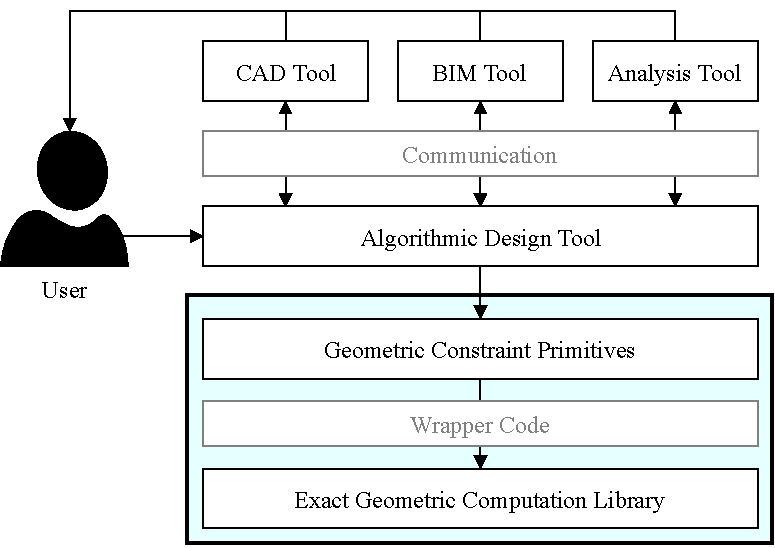
\includegraphics[width=\textwidth]{fig/solution-arch}
  \caption[Solution architecture within AD workflow]{
    General overview of the solution's architecture encapsulated within the
    blue colored box beneath a depiction of the typical \ac{AD} workflow.}%
  \label{fig:solution.arch}
\end{figure}

The following sections go over the components in \cref{fig:solution.arch},
namely the \geomlibrary{}, the \wrapper{}, and the \primitives{}.  Additionally,
we discuss a few trade-offs from tackling the problem in this fashion as opposed
to potential alternative routes, describing advantages and disadvantages of our
approach.

% !TEX root = ../../main.tex
\section{Implementation}%
\label{sec:solution.impl}

This section details implementation choices with regard to the chosen platforms
for realizing the initially proposed general solution architecture, previously
illustrated in \cref{fig:solution.arch}. Following a brief analysis, we expand
specifically on the concrete components corresponding to the ones within
\cref{fig:solution.arch}'s light blue rectangle.

Examining the \ac{AD} workflow portion of \cref{fig:solution.arch}, there are
depictions of \ac{CAD}, \ac{BIM}, and analysis tools, of which examples could be
Rhinoceros3D, Autodesk's Revit, and Radiance, respectively, with no particular
focus on any of them.  Digging a layer deeper, we find the \ac{AD} tool, which,
by means made available by the tools above it, produces models specific to those
tools from a description provided by the user.  The \ac{AD} tool we have chosen
was
Khepri\footnote{\url{https://github.com/aptmcl/Khepri.jl}}~\cite{Leitao:2019:GRUGEAV},
a text-based tool written in the Julia programming
language~\cite{Bezanson:2017:JAFANC}.  Khepri is the successor of another
text-based \ac{AD} tool named Rosetta~\cite{Leitao:2011:PGDCAD}, a tool written
in the Racket programming language~\cite{PLT:2010:Reference}.  It follows that
the \primitives{} were implemented in the Julia language as well, supported by
an \geomlibrary{}.  The library chosen for the effect was
\ac{CGAL}~\cite{CGAL:5.3:Project}, a highly performant and robust geometric
library written in the C++ programming language~\cite{Stroustrup:2013:CPP}.
\Ac{CGAL} is a comprehensive, mature, open-source library, offering plenty of
data structures and functionality of varying complexity, focusing to provide
easy access to efficient and reliable geometric algorithms.

The language disparity between the \primitives{} module (Julia) and the
\geomlibrary{} (C++) requires a solution for language interoperation.  In other
words, we need to make \ac{CGAL} available to the Julia language.  The Julia
language already possesses facilities that invoke functionality within libraries
written in the C~\cite{Kernighan:1988:C} or the
Fortran~\cite{Backus:1957:Fortran} programming languages, an interfacing
mechanism is commonly known as \ac{FFI}.  It allows for the repurposing of
mature software libraries in foreign languages without the need for a complete
rewrite or adaptation.\footnote{The decision to include such a mechanism at the
language's core by the language designers makes it so that the language can gain
traction early, biding time to later explore native implementations.  Arguably,
it may be one of \textit{the} fundamental features that made the language as
popular as it is and kept it afloat, unlike other similar historical examples
that might have lacked such a mechanism.}  Despite only addressing libraries
written in C and Fortran, this mechanism can also in turn be leveraged and built
upon to interface with other programming languages, e.g., Java, Python, MATLAB,
and, C++.\footnote{There is an entire GitHub organization with projects
dedicated to foreign language interoperation at
\url{https://github.com/JuliaInterop} (July 8, 2021)}

Overcoming the language interoperability hurdle, we can now start focusing on
the implementation of the \primitives{}.  These primitives build on top of the
functionality available in \ac{CGAL}, some of which is directly inherited from
it, substantially helping us in the process.  We further enriched the pool with
a few more functions, illustrating a constructive approach to \ac{GCS}, similar
and inspired by the approach of \texttt{tkz-euclide}, mentioned in
\cref{sec:related.constraints.tikz}.  By creating an abstraction over more
primitive functionality, we aimed to provide an easy to understand and utilize
set of tools so that users can avoid the error-prone process of reimplementing
it themselves.  Furthermore, we level the playing field by working at a
conceptual level which is more familiar to traditional \ac{CAD} software users
rather than falling back to the more analytic approach programming languages
naturally offer.

The following sections will elaborate further on the components emphasized in
the previous paragraphs, adopting a bottom-up-like approach.  We will discuss
\ac{CGAL} and what constructs and functionality it can provide to aid our goal,
as well as some added benefits of building on top of a very mature and
comprehensive library.  That will be followed by a section detailing how it was
possible to map said functionality to the Julia language, of which the result
was a Julia package aptly named \texttt{CGAL.jl}\footnote{Packages in the Julia
ecosystem are conventionally terminated with a \texttt{.jl} suffix, the
extension used for Julia files.  This is reminiscent of a familiar convention
followed in the Java ecosystem where libraries and tools are usually prefixed
with the letter \texttt{J}, e.g., \texttt{JUnit}, \texttt{JMeter},
\texttt{JDeveloper}, among others.}~\cite{Ventura:2021:CGAL.jl}.  Finally, we
showcase how we leveraged \texttt{CGAL.jl} to build the aforementioned
\primitives{}, a set of functionalities that implements specialized yet
comprehensible constructive approach solutions to \ac{GC} problems.

% !TeX root = ../../../main.tex
\subsection{Computational Geometry Algorithms Library}%
\label{sec:solution.impl.cgal}

\Ac{CGAL} is a software project that provides easy access to efficient and
reliable geometric algorithms in the form of a C++ library.  It is considered
the industry's \textit{de facto} standard geometric library, used in well-known
projects such as OpenSCAD\@.  It is also a very mature software library with
decades of Ph.D.-grade research results, still being actively maintained to this
day.  Being an open-source project, one can easily contribute to it by reporting
issues in the software as well as directly submitting patches.\footnote{The
library's source is hosted on GitHub at \url{https://github.com/CGAL/cgal}.  To
illustrate the ease with which one can contribute to the project, here is a pull
request the author submitted: \url{https://github.com/CGAL/cgal/pull/4705}.}

These factors, among others, justify our choice for our solution's
\geomlibrary{} component: we chose \ac{CGAL} because of its comprehensiveness
and decades of work invested in the production of a piece of highly mature
software, as well as the critical mass of maintainers behind it.  That is not to
say less mature software cannot be used in its stead, though it is unlikely it
can match \ac{CGAL}, be it in terms of performance, quality, or breadth.

\ac{CGAL} offers a multitude of data structures and algorithms, such as
triangulations, Voronoi diagrams, and convex hull algorithms, to name a few.
The library is broken up into three parts~\cite{CGAL:5.3:23LGK}:
\begin{enumerate}
  \item The kernel, which consists of geometric primitive objects and operations
  on these objects.  The objects are represented both as
  \begin{enumerate*}
    \item stand-alone classes parameterized by a representation class that
    specifies the underlying number types used for computation, and as
    \item members of the kernel classes, which allows for more flexibility and
    adaptability of the kernel;
  \end{enumerate*}
  \item Basic geometric data structures and algorithms, parameterized by traits
  classes that define the interface between the data structure or algorithm and
  the primitives they use;
  \item Non-geometric support facilities, such as circulators, random sources,
  and I/O support for debugging and for interfacing \ac{CGAL} with various
  visualization tools.
\end{enumerate}

Kernels in \ac{CGAL} are parametric, enabling the combination of kernels with
exact constructions or inexact constructions.  The latter are faster than the
former, but may produce inexact results due to \textit{roundoff} errors during
object construction.  In practice, however, inexact construction kernels suffice
for most of \ac{CGAL}'s algorithms.

\Cref{lst:solution.impl.cgal.pas} showcases an example of a very simple
\ac{CGAL} program, demonstrating the construction of points and a segment, and
performing some basic operations on them.

\begin{listing}[htbp]
  \caption[CGAL: Three points and one segment]{
    An example CGAL program illustrating how to construct some points and a line
    segment, and perform some basic operations on them.  It uses
    \mintinline{c}{double} precision floating point numbers for Cartesian
    coordinates.}\label{lst:solution.impl.cgal.pas}
  \inputminted{cpp}{cpp/points_and_segments.cpp}
\end{listing}

As mentioned, geometric primitive types are defined in the kernel.  The kernel
chosen in the example uses \texttt{double} precision floating point numbers for
the Cartesian coordinates of the point.

We can also see some predicates, such as testing the orientation of three
points, and constructions, like the distance\footnote{It is worth noting
\ac{CGAL} does \texttt{not} compute the absolute distance, offering instead to
compute the squared distance, as this avoids the additional square root
computation.  This preserves exactness and eliminates a potentially unnecessary
heavy computation.} and midpoint computation.  Predicates typically produce a
boolean logical value or one of a discrete set of possible results, whereas
constructions produce either a number or another geometric entity.

It is worth noting that floating point-based geometric computation can lead to
surprising results since we are relying on inexact constructions.  If one must
ensure that the numbers get interpreted at their full precision, all one has to
do is pick a kernel with exact constructions.  Revisiting
\cref{lst:solution.impl.cgal.pas}, it is as simple as switching the
\texttt{Simple\_cartesian} kernel with one the provides exact constructions,
e.g., \texttt{Exact\_predicates\_exact\_constructions\_kernel} or \texttt{Epeck}
for short.

Unfortunately, \ac{CGAL} is a terribly complex library under the hood,
presenting many challenges when it comes to mapping it to the Julia language.
Firstly, it is a C++ library.  Despite Julia's native capabilities for
interoperating with C, there's additional work to be done to reach C++ code.
Secondly, is problem of memory management, which differs between C/C++ and
Julia, potentially leading to memory leaks and other related issues if not
properly tended to.  Finally, \ac{CGAL} makes extensive use of C++ templates,
proving sometimes difficult to transparently map some of its constructs.

In the next section, we go over how we overcame these issues.

% !TeX root = ../../../main.tex
\subsection{From C++ to Julia}%
\label{sec:solution.impl.jlcgal}

Having established \ac{CGAL} as our \geomlibrary{} of choice, we must now
overcome the quite literal language barrier between Julia and C++.  Fortunately,
the former possesses \ac{FFI} mechanisms that can aid us in resolving this
issue.  Here is an excerpt from the language's manual about Julia's C and
Fortran \ac{FFI} capabilities:\footnote{From
\url{https://docs.julialang.org/en/v1/manual/calling-c-and-fortran-code/}}

\begin{quote}
  \itshape\color{gray}
  To allow easy use of (\ldots) existing code, Julia makes it simple and
  efficient to call C and Fortran functions.  (\ldots) This is accomplished just
  by making an appropriate call with \mintinline{julia}{ccall} syntax, which
  looks like an ordinary function call.
\end{quote}

To illustrate how this \mintinline{julia}{ccall} construct can be used in the
context of our problem, we created a small wrapper around \ac{CGAL} exposing the
\texttt{squared\_distance} function whose signature can be seen in
\cref{lst:solution.impl.jlcgal.sqdist.sig}.
\begin{listing}[htb]
  \begin{minted}[linenos=false]{cpp}
    template<typename Kernel>
    Kernel::FT squared_distance(Type1<Kernel> obj1, Type2<Kernel> obj2) 
  \end{minted}
  \caption[\texttt{squared\_distance} function signature]{
    Function signature of \ac{CGAL}'s \texttt{squared\_distance} global
    function.  \texttt{Type1} and \texttt{Type2} can be, among several objects,
    \texttt{Point\_3}s.}%
  \label{lst:solution.impl.jlcgal.sqdist.sig}
\end{listing}
To facilitate the wrapping, we create the points on the C++ side of things,
instead passing primitive \mintinline{cpp}{double} values representing the
points' coordinates.  The C++ wrapper library is shown in
\cref{lst:solution.impl.jlcgal.sqdist.cpp}.

\begin{listing}[htb]
  \inputminted{cpp}{cpp/sqdist.cpp}
  \caption[C wrapper for squared distance functionality]{
    Example C library code that wraps \ac{CGAL}'s \texttt{squared\_distance}
    global function.  The original function takes in instances of
    \texttt{Point\_3} classes, so we instantiate them from our
    \mintinline{cpp}{double} coordinate inputs.}%
  \label{lst:solution.impl.jlcgal.sqdist.cpp}
\end{listing}

To invoke our wrapper function, we must precede it with \mintinline{cpp}{extern
"C"}, as is illustrated, to make it accessible as a C function from the
perspective of Julia.  This is important because C++ compilers mangle function
names.  Name mangling is employed to solve a series of problems in order to
support features like function overloading. By preventing it from happening, we
can then refer to our wrapper function by its declared name, just like a C
function.

After compiling the library, we can invoke the newly wrapped function from Julia
using \mintinline{julia}{ccall}, as showcased in
\cref{lst:solution.impl.jlcgal.sqdist.jl}.

\begin{listing}[htb]
  \inputminted{julia}{jl/sqdist.jl}
  \caption[Julia squared distance example program]{
    Example Julia program that invokes the functionality from the library whose
    source is listed in \cref{lst:solution.impl.jlcgal.sqdist.cpp}.  Julia's
    \mintinline{julia}{ccall} construct converts the input arguments' types to
    the types specified in the native C function's parameter types.}%
  \label{lst:solution.impl.jlcgal.sqdist.jl}
\end{listing}

Though this looks like a good start, the number passing strategy soon shows its
limitations, particularly, due to the combinatorial explosion problem that may
arise when a function requires a number $M$ of $N$-dimensional points.  We would
then have to create a wrapper that takes $N\cdot M$ coordinates,  an approach
that clearly does not scale.  Fortunately, it is possible to overcome this
limitation by mirroring C \mintinline{cpp}{struct}s in Julia.

As an example, we consider the \texttt{circumcenter} function from \ac{CGAL}.
Specifically, the function that takes three points as its parameters, returning
the circumcenter about the given points, under the assumption the points are not
collinear.  The function signature can be seen in
\cref{lst:solution.impl.jlcgal.circ.sig}.  
\begin{listing}
  \begin{minted}[linenos=false]{cpp}
    template<typename Kernel> 
    Point_3<Kernel> circumcenter(const Point_3<Kernel>& p,
                                 const Point_3<Kernel>& q,
                                 const Point_3<Kernel>& r)
  \end{minted}
  \caption[\texttt{circumcenter} function signature]{
    Function signature of \ac{CGAL}'s \texttt{circumcenter} global function that
    takes three input \texttt{Point\_3}s.}%
  \label{lst:solution.impl.jlcgal.circ.sig}
\end{listing}
We could try and directly mirror
\ac{CGAL}'s \texttt{Point\_3} type, but that would require that we know its
layout.  Even then, we would be breaking an abstraction barrier that could prove
detrimental if \ac{CGAL}'s developers decide to change the type's internal
representation.  To circumvent this completely, we can just create a
\mintinline{cpp}{struct} that opaquely wraps around \ac{CGAL}'s type.  The C++
wrapper code for this example is listed in
\cref{lst:solution.impl.jlcgal.circ.cpp}.

\begin{listing}[htbp]
  \inputminted{cpp}{cpp/circ.cpp}
  \caption[C wrapper for circumcenter functionality]{
    Example C shared library source code that wraps \ac{CGAL}'s circumcenter
    global function.  In this instance, we use an additional struct to wrap
    around \ac{CGAL}'s \texttt{Point\_3} class to facilitate data transfer.}%
  \label{lst:solution.impl.jlcgal.circ.cpp}
\end{listing}

The wrapper code looks very similar to the previous example in
\cref{lst:solution.impl.jlcgal.sqdist.cpp}.  This time, however, we introduced a
new \mintinline{cpp}{struct Point} that we will mirror in Julia so that we can
seamlessly pass instances of it to our externalized C++ function.\footnote{Note
that, unlike the function, the \mintinline{cpp}{struct} was not externalized.
This is not necessary because we do not need to refer it by name.  We need only
to match its field layout.}  All the wrapper function does is take in our
\texttt{Point}s and create new \texttt{Point\_3} objects, using them to invoke
\ac{CGAL}'s \texttt{circumcenter} function.  The returned \texttt{Point\_3} is
then used to create a \texttt{Point}, which is later sent back upstream to
Julia.

On the Julia side of things, the process is much the same as before with the
addition of a new \texttt{Point} type that contains three
\mintinline{julia}{Float64} fields. The previous example showed the latter Julia
type's correspondence to the C/C++ \mintinline{cpp}{double} type.  The Julia code
for this example is listed in \cref{lst:solution.impl.jlcgal.circ.jl}.

\begin{listing}[htb]
  \inputminted{julia}{jl/circ.jl}
  \caption[Julia circumcenter example program]{
    Example Julia program that invokes the functionality from the library listed
    in \cref{lst:solution.impl.jlcgal.circ.cpp}.  We use an additional Julia
    struct that is equivalent to the one specified in C to facilitate data
    transfer.}%
  \label{lst:solution.impl.jlcgal.circ.jl}
\end{listing}

We are once again met with a very familiar snippet of code.  Much like with its
respective wrapper library, there is a new \mintinline{julia}{struct Point} that
mirrors the one we created in C++.  From then on, the process is exactly the
same.

So far, we were able to extract two useful functions from \ac{CGAL}.  In fact,
the second one already solves the problem exemplified in a previous chapter in
\cref{sec:intro.examples.circumcenter}.  Although we could incrementally build
upon this approach, not only does it become cumbersome, but it proves
impractical, given \ac{CGAL}'s complexity.

Fortunately, the Julia community has explored methods of interoperating with
many other languages, one of them being C++.  That exploration resulted in
packages like 
\texttt{CxxWrap.jl}.\footnote{\url{https://github.com/JuliaInterop/CxxWrap.jl}}
\texttt{CxxWrap.jl} adopts an approach to language interoperation similar to
that of BOOST.Python~\cite{Abrahams:2003:BHSBP} or
pybind11.\footnote{\url{https://github.com/pybind/pybind11}}  The user writes
the code for the Julia wrapper in C++, and then simply issues an instruction on
the Julia side to initialize the library, making it available there.  The Julia
package is supported by a C++ component known as \texttt{libcxxwrap-julia}, or
the friendlier name JlCxx. This component is what the C++ wrapper code depends
on.  \Cref{lst:solution.impl.jlcgal.jlcxx} constitutes the code to wrap
necessary functionality to reproduce the example \ac{CGAL} program in
\cref{lst:solution.impl.cgal.pas}.

\begin{listing}[htbp]
  \caption[Wrapper CxxWrap code for Three points and one segment]{
    C++ wrapper code powered by JlCxx that maps the types and functions needed
    from \acs{CGAL} to reproduce the example shown in
    \cref{lst:solution.impl.cgal.pas} in Julia.}%
  \label{lst:solution.impl.jlcgal.jlcxx}
  \inputminted[fontsize=\small]{cpp}{cpp/cgal_julia.cpp}
\end{listing}

We direct our focus to the lines that are highlighted in
\cref{lst:solution.impl.jlcgal.jlcxx}.  We define a function that is later
invoked by \texttt{CxxWrap.jl}.  In it, we start registering the required types
and functions that we need in a declarative fashion,\footnote{Order with which
types and functions are registered matters.  This means we cannot add a function
that depends on a type we did not yet register.} reminiscent of the builder
design pattern~\cite{GOF:1994:DPEROOS}.  Notice the \texttt{JLCXX\_MODULE}
symbol preceding the function definition.  That symbol takes care of properly
externalizing the function regardless of the system the library is built
for.\footnote{Think similar to \mintinline{cpp}{extern "C"}, but slightly more
robust.}

After compiling the wrapper code, we can load it on the Julia side resorting to
\texttt{CxxWrap.jl}.  This process is reminiscent of and analogous to the ones
illustrated earlier with simpler examples using \mintinline{julia}{ccall}.
\Cref{lst:solution.impl.jlcgal.cgal} shows a bare-bones CGAL Julia module.

\begin{listing}[htbp]
  \inputminted{julia}{jl/CGAL.jl} 
  \caption[Bare-bones Julia module wrapping some of CGAL]{
    An example Julia module that mimics \texttt{CGAL.jl}, wrapping the library
    produced from \cref{lst:solution.impl.jlcgal.jlcxx}.  It initializes the
    library and exports the mapped functionality.}%
  \label{lst:solution.impl.jlcgal.cgal}
\end{listing}

All that is necessary to make the functionality we wrapped on the C++ side
available to Julia is
\begin{enumerate*}[label= (\arabic*)]
  \item tell \texttt{CxxWrap.jl} where the library is,
  \item tell \texttt{CxxWrap.jl} to initialize itself when the module is loaded,
  and
  \item export the mapped functionality.
\end{enumerate*}
The rest of the non-highlighted code, both in this example and the previous
only serves the purpose of obtaining a human-readable representation of the C++
objects in Julia.

Finally, we reach a point where we are able to reproduce the example listed in
\cref{lst:solution.impl.cgal.pas} in the Julia language, having mapped all the
necessary functionality to do so.  \Cref{lst:solution.impl.jlcgal.pas} shows the
example, translated from C++.

\begin{listing}[htb]
  \inputminted{julia}{jl/points_and_segments.jl}
  \caption[CGAL.jl: Three points and one segment]{
    The example program as seen in \cref{lst:solution.impl.cgal.pas} written in
    the Julia programming language using \texttt{CGAL.jl}.  The kernel
    instantiation is hidden away in the C++ layer of the wrapper code.}%
  \label{lst:solution.impl.jlcgal.pas}
\end{listing}

We illustrated how to repurpose some core functionality on which we can continue
to incrementally build upon following a similar approach to that shown in
\cref{lst:solution.impl.jlcgal.jlcxx}.  Doing so, with relatively low effort, we
can obtain the primitive objects and functionality on which our \primitives{}
will be supported.  The following section goes over how we effectively used the
functionality from \texttt{CGAL.jl} to implement constructive solutions for
\ac{GC} problems.

% !TeX root = ../../../main.tex
\subsection{Geometric Constraint Primitives}%
\label{sec:solution.impl.gcps}

Having overcome the language barrier between C++ and Julia, we can build our
\ac{GC} primitives on top of \texttt{CGAL.jl}.  Our implementation of the
\primitives{} is loosely inspired on tools like \texttt{tkz-euclide} and
Eukleides.  Both are based on Euclidean geometry, a constructive system where
the production of geometry can be done solely resorting to a straightedge and a
compass.  This makes programs described using these constructs easier to
understand and manually reproduce.

The following sections include a revisiting of our initially formulated example 
problems, described in \cref{sec:intro.examples}, and another set of primitives
that will be the driving force behind the case studies we go over later in
\cref{chap:eval}.

\subsubsection{Parallel lines}%
\label{sec:solution.impl.gcps.parallel}

Revisiting our earlier examples, we now showcase implementations for those
problems using our solution, accompanied by visualizations resorting to the
Khepri \ac{AD} tool.  \Cref{lst:solution.impl.gcps.parallel} shows a solution to
the ``parallel lines'' problem introduced in \cref{sec:intro.examples.parallel}.

\begin{listing}[htbp]
  \inputminted{julia}{jl/ex_parallel.jl}
  \caption[Parallel lines example using our solution]{
    Implementation of the parallel lines example illustrated in
    \cref{fig:intro.example.parallel} using Khepri alongside our solution.}%
  \label{lst:solution.impl.gcps.parallel}
\end{listing}

The sixth line in the program consists of the implementation of the primitive
construct.  The \texttt{parallel} function takes a line segment \texttt{l}, the
segment the resulting line is meant to be parallel to; and a point \texttt{p}
which the resulting line passes through.  We then build a new line segment whose
starting point is the given point \texttt{p}, and the end point is the result of
adding the difference between \texttt{l}'s endpoints to \texttt{p}, obtained
using \texttt{CGAL.jl}'s \texttt{to\_vector} function.

We then need to tell Khepri how to create objects our implementation can
understand by converting both the inputs and the resulting output.
\texttt{CGAL.jl} already contains a primitive shim of conversions between some
objects that facilitate this effort.\footnote{Ideally, the target \ac{AD} tool
would integrate our solution's constructs in a tighter more seamless fashion.}

Finally, we can use our primitive as seen in the listing's eighteenth line,
reproducing the same result. \Cref{fig:solution.impl.gcps.parallel} illustrates
the formulated program's output in AutoCAD, one of the visualization tools
Khepri supports.

\begin{figure}[htbp]
  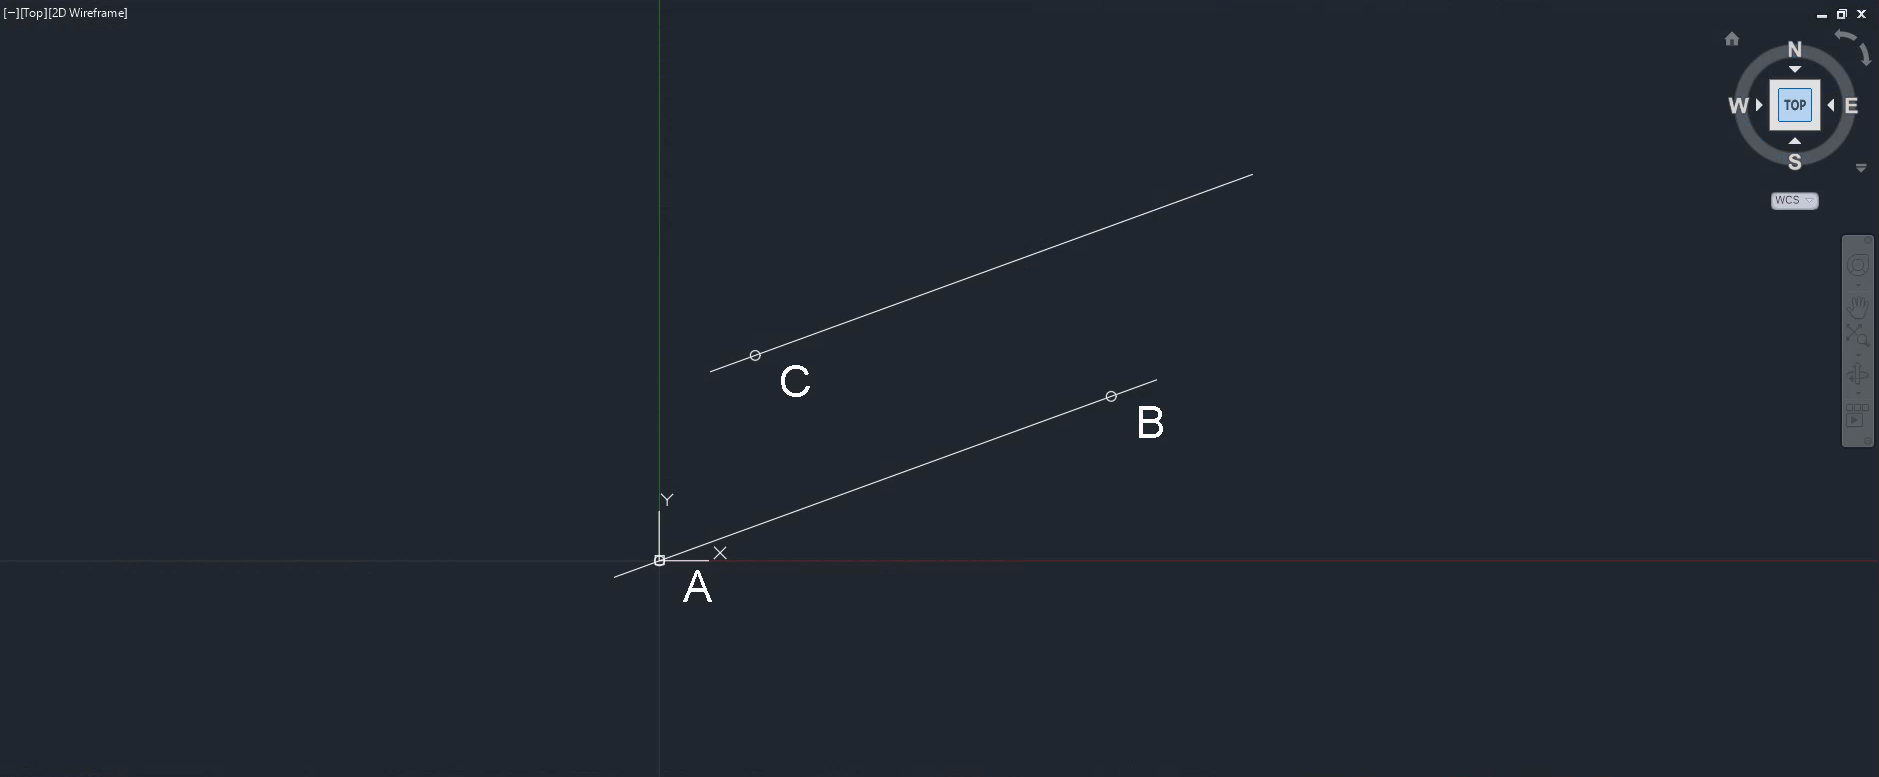
\includegraphics[width=\linewidth]{fig/autocad-parallel} 
  \caption[Parallel lines example using our solution]{
    Parallel lines example from \cref{sec:intro.examples.parallel} revisited
    using our solution's \texttt{parallel} primitive construct.  Output
    visualized in AutoCAD.}%
  \label{fig:solution.impl.gcps.parallel}
\end{figure}

\subsubsection{Circumcenter}%
\label{sec:solution.impl.gcps.circumcenter}

Regarding our circumcenter problem, introduced in
\cref{sec:intro.examples.circumcenter}, we initially solved it by intersecting
two of the three triangle sides' bisectors.  We can still approach the problem
that way, defining a \texttt{circumcenter} function similar to the one in
\cref{lst:solution.impl.gcps.circimpl}.

\begin{listing}[htbp]
  \begin{minted}[linenos=false]{julia}
  circumcenter(a, b, c) = intersection(bisector(a, b), bisector(b, c)) 
  \end{minted}
  \caption[Initial circumcenter solution]{
    Initial implementation of the \texttt{circumcenter} function.}%
  \label{lst:solution.impl.gcps.circimpl}
\end{listing}

However, this is one occasion where this functionality is already present in
\ac{CGAL}.  This is a simple yet perfect demonstration of one of our approach's
benefits with regard to repurposing a comprehensive library with plenty of
functionality, allowing us near-direct reuse without re-implementing it.

\Cref{lst:solution.impl.gcps.circumcenter} illustrates a solution to the
``circumcenter'' problem using \ac{CGAL}'s \texttt{circumcenter} function.  The
program's output can be seen in \cref{fig:solution.impl.gcps.circumcenter}.

\begin{listing}[htbp]
  \inputminted{julia}{jl/ex_circumcenter.jl}
  \caption[Circumcenter example using our solution]{
    Implementation of the circumcenter example illustrated in
    \cref{fig:intro.example.circumcenter} using Khepri alongside our solution.}%
  \label{lst:solution.impl.gcps.circumcenter}
\end{listing}

\begin{figure}[htbp]
  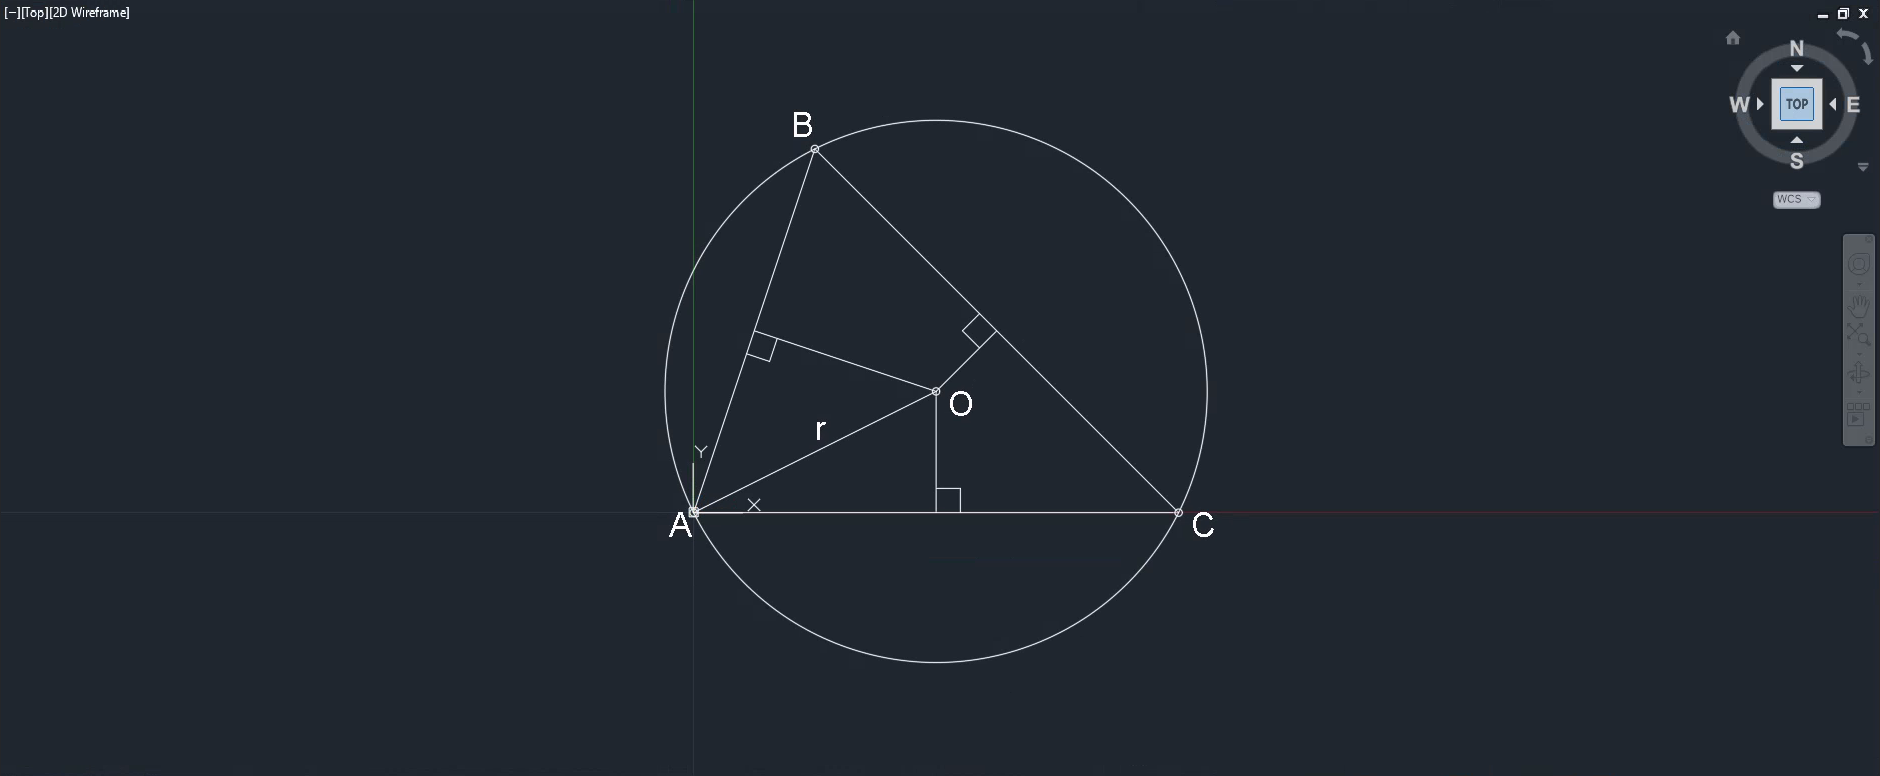
\includegraphics[width=\linewidth]{fig/autocad-circumcenter} 
  \caption[Circumcenter example using our solution]{
    Circumcenter example revisited using our solution's \texttt{circumcenter}
    primitive construct.  Output visualized in AutoCAD.}%
    \label{fig:solution.impl.gcps.circumcenter}
\end{figure}

\subsubsection{Circle tangent to a line}%
\label{sec:solution.impl.gcps.tangcirc2line}

Moving on to a set of problems that cannot as directly be solved by \ac{CGAL} is
that of tangencies.  Generally speaking, there are specific constructs available
in \ac{CGAL} that solve these problems.  However, we can once again repurpose
the ones we have and build on top of them.

This problem involves computing a circle that is tangent to an already existing
line.  Given the circle's center \texttt{o} and the line \texttt{l} we want the
circle to be tangent to, the tangent circle is such that its radius is the
minimal distance between its center point \texttt{o} and the line \texttt{l}.
The implementation of the problem's solution can be seen in
\cref{lst:solution.impl.gcps.tangcircle2line}.

\begin{listing}[htb]
  \begin{minted}[linenos=false]{julia}
  tangent_circle(o::Point2, l::Line2) = Circle2(o, squared_distance(o, l))
  \end{minted}
  \caption[Circle tangent to a line]{
    Implementation of the ``Circle tangent to a line'' problem.}%
  \label{lst:solution.impl.gcps.tangcircle2line}
\end{listing}

Notice this solution considers we are working with infinite lines, not
necessarily line \textit{segments} in general.  Were we to apply the same simple
approach to a line segment, the circle would end up tangent to the line segment
as well.  However, the resulting circle could be tangent to one of the segment's
endpoints instead of tangent to a point along the segment.  In some cases, the
latter behavior may be preferred, for which adjustments to the solution must be
made, such as indicating that there is no solution for the given center point.

We did not implement such a scenario regarding line segments, because much like
the other primitives, it was created to satisfy a specific use case's
requirements.  A potential solution to that specific problem could be obtained
reusing the \texttt{tangent\_circle} function, however.  We would then need to
verify if the circle would fall somewhere between the segment's endpoints.
Otherwise, there would not be a solution available.

\subsubsection{Tangent circles}%
\label{sec:solution.impl.gcps.tangentcircles}

Another instance of tangency is that of two circles tangent to each other.  This
proves to be a relatively more complex problem due to how the circles may be
positioned.

Given two circles \texttt{c\textsubscript{1}} and \texttt{c\textsubscript{2}},
and a vector \texttt{v} used to indicate the point of tangency on
\texttt{c\textsubscript{1}}, we draw a circle centered on said point with the
same radius as \texttt{c\textsubscript{2}} and intersect it with a ray
\texttt{r'} originating from the former circle's center, giving us a point
\texttt{f}.  This ray may be directed in one of two ways, determining if the
resulting circle contains both circles or not.  We then compute the bisector
\texttt{b} between \texttt{f} and \texttt{c\textsubscript{2}}.  We test if we
are in a situation where the resulting circle would instead turn out to be a
line.  If that is the case, we produce an error.  Otherwise, we construct the
tangent circle.

\Cref{lst:solution.impl.gcps.tangentcircles} contains the solution to the
problem, assisted by our own definition of the intersection function between a
circle and a ray, listed in \cref{lst:solution.impl.gcps.circrayint}.

\begin{listing}[htb]
  \inputminted[firstline=11]{julia}{jl/tangent_circles.jl}
  \caption[Tangent circles]{
    Implementation of the ``Tangent circles'' problem.}%
  \label{lst:solution.impl.gcps.tangentcircles}
\end{listing}

\begin{listing}
  \inputminted[lastline=9]{julia}{jl/tangent_circles.jl}
  \caption[Circle-Ray intersection]{
    Implementation of the intersection between a circle and a ray.}%
  \label{lst:solution.impl.gcps.circrayint}
\end{listing}

\subsubsection{Tangent lines between circles}%
\label{sec:solution.impl.gcps.tanglines2circles}

Another problem that surfaced in a case study earlier illustrated in
\cref{fig:intro.chair} is that of computing tangent lines between two circles.
It is a slightly more complex problem for which there is no obvious solution.
Fortunately, a constructive solution to this problem already
exists,\footnote{\url{https://en.wikipedia.org/wiki/Tangent_lines_to_circles\#Synthetic_geometry}}
an approach our implementation is based on.

This problem's complexity lead us to break it into two different problems.
First, we must determine the lines tangent to a circle that pass through a given
point (\cref{lst:solution.impl.gcps.tanglines2circles}).  Then, repurposing the
solution to that problem, we solve the overarching problem of determining the
lines tangent between circles (\cref{lst:solution.impl.gcps.tanglines2circle}).
This is another example of how we can compose a smaller set of primitives to
solve a larger problem.

\begin{listing}[htbp]
  \inputminted[firstline=2,lastline=16]{julia}{jl/circ_tangent_lines.jl}
  \caption[Tangent lines to a circle]{
    Implementation of the ``Tangent lines to a circle'' sub-problem.}%
  \label{lst:solution.impl.gcps.tanglines2circles}
\end{listing}

\begin{listing}[htbp]
  \caption[Tangent lines between circles]{
    Implementation of the ``Tangent lines between circles'' problem by way of
    composition with the solution of ``Tangent lines to a circle''.}%
  \label{lst:solution.impl.gcps.tanglines2circle}
  \inputminted[firstline=18,lastline=59]{julia}{jl/circ_tangent_lines.jl}
\end{listing}

Our implementation returns the results in a deterministic way, facilitating
result choice.  The line segments are oriented from \texttt{c\textsubscript{1}}
to \texttt{c\textsubscript{2}}, with the internal tangents surrounded by the
external tangents, sorted in a counterclockwise orientation.


% !TeX root = ../../main.tex
\section{Trade-offs}%
\label{sec:solution.tradeoffs}

Since virtually nothing comes without trade-offs and compromises, it is
paramount we address our implementation's qualities, both negative and positive.

Relying on a library such as \ac{CGAL} proves to be as great as it can be
daunting.  As mentioned in \cref{sec:solution.impl.cgal}, \ac{CGAL} is a very
comprehensive and mature software library, arguably even far exceeding our
solution's needs, yet fitting it perfectly.

It is, however, an external component, and with every such component, we do not
hold as much control over it as if it was internal instead.  For example, in the
advent a bug is found within \ac{CGAL}, one cannot \emph{immediately} fix it by
altering its source code and use this fixed version.\footnote{Not unless one
wishes to maintain an entirely separate version of the software until this local
fix is applied upstream.  It can be tiresome if we wish to distribute our
solution and have to redistribute a different version of \ac{CGAL} as well
instead of the globally available releases.}  Important emphasis on bugs not
being \emph{immediately} fixable lest we forget \ac{CGAL} is still an
open-source project arguably anyone can contribute to.  Alas, said contribution
deployments are still out of our control.  In hindsight, however, it can be
considered as just an inconvenience since it is a project that is actively
maintained by very knowledgeable people in the computer graphics and mathematics
fields.

\Ac{CGAL} is also a highly generic library, making heavy use of C++ templates.
Although its design makes usage an elegant experience, the same cannot be said
when trying to map its constructs to another language, especially a language
with a different memory management paradigm which could lead to some nasty
low-level ordeals.  Luckily, \texttt{CxxWrap.jl} helps us solve most, if not
all, of those issues.

Regarding our wrapper code, there is one small problem we still technically did
not solve.  We are still mapping \ac{CGAL} types in an opaque fashion, fixing
the kernel on the C++ side.\footnote{There are other projects that attempt to
make \ac{CGAL} available in other language that resort to this same trick. See
\url{https://github.com/scikit-geometry/scikit-geometry} and
\url{https://github.com/CGAL/cgal-swig-bindings}.}  Alternative methods of
supplying a different kernel were explored, including deploying a different
library compiled with a different kernel.  Despite not entirely solving the
problem, it offered the user the choice of using exact constructions.  However,
this alternative became unmaintainable and virtually impossible to successfully
employ.  In part due to Julia's package pre-compilation, it is no longer viable
to use this other library.

Ideally, the geometric objects would be parametric, and the kernel (or kernels)
mapped to Julia as well, but we were met with complications that would make it
unfeasible for us to implement our solution.  As a compromise, \texttt{CGAL.jl}
fixed a kernel that provides exact predicates with inexact constructions,
favoring performance over some robustness loss.  Nonetheless, in practical
terms, it suffices for our case.

As an alternative to wrapping \ac{CGAL}, we could have explored other options in
the still growing Julia ecosystem.  Some work seems
promising,\footnote{\url{https://github.com/JuliaGeometry}} but not only are
some libraries still catching up, it is also highly unlikely they will ever meet
the quality of \ac{CGAL}.

Lastly, some of our \ac{GC} primitives employ some computation that can lead to
robustness loss as well.  Primarily the ones that involve circles, non-linear
geometric objects, typically require the computation of a square root to work
with absolute distances.  We typically avoid those computations, postponing them
as much as possible until they are absolutely necessary.  As an example, in the
``tangent lines to a circle'' implementation in
\cref{lst:solution.impl.gcps.tanglines2circles}, we first compare squared
distances before requiring their absolute value.

Be that as it may, due to having fixed a kernel with inexact constructions for
\ac{CGAL}, we are bound with some robustness loss regardless.  At this point, it
can only be mitigated by also ensuring the quality of the inputs given to our
primitives, and that is reliant on the user.  If the user decides to provide
``garbage'' inputs, they will most likely be met with ``garbage'' outputs, a
concern, however, that falls out of the scope of this work.


% !TEX root = ../main.tex
\fancychapter{Evaluation}%
\label{chap:eval}
\cleardoublepage{}

\noindent In this chapter, we evaluate our solution by measuring the qualities
of the approach we took to tackle \ac{GCS}.

Firstly, we aim to benchmark our solution's performance by comparing it to a
similar project called ConstraintGM~\cite{Pinheiro:2016:MGR}.  We were able to
reproduce the project's original benchmark tests and create an analogous test
suite for our solution so we can compare both projects.

Secondly, we showcase four different case studies inspired by existing designs.
This section of the evaluation focuses on comparing different approaches to
solving \ac{GC} problems present in each case study by adopting two different
approaches: 
\begin{enumerate*}[label= (\arabic*)]
  \item an analytic approach, one programming naturally begs for, and 
  \item a constructive approach, essentially adding a conceptual abstraction
  layer over the former.
\end{enumerate*}
We aim to show that, by following the latter approach, resulting programs become
both easier to understand and reproducible as the set of instructions can be
used to recreate the resulting geometry by hand, using a ruler and a compass.

Finally, as an added bonus, we explore our approach's potential regarding
repurposing more complex geometric algorithms, contrasting it with
re-implementing a version of said algorithms from scratch.  Specifically, we set
out to repurpose \ac{CGAL}'s 2D Delaunay Triangulation and Voronoi Diagram
algorithms and further compare the resulting mapping's performance and
correctness when compared to a native Julia implementation of the algorithms as
provided by the package
\texttt{VoronoiDelaunay.jl}\footnote{\url{https://github.com/JuliaGeometry/VoronoiDelaunay.jl}},
that, in the past, was once benchmarked against
\ac{CGAL}.\footnote{\url{https://gist.github.com/skariel/3d2018f9341a058e00fc}}
Additionally, we set out to estimate the effort it took to develop
\texttt{VoronoiDelaunay.jl} and compare that to the effort it took to extract an
analogous algorithm from \ac{CGAL}.

Benchmarks were performed on a Lenovo{\textregistered}
ThinkPad{\textregistered} E595 laptop computer with the following
system specifications:

\begin{itemize}
  \item \acsu{AMD}\label{acro:AMD} Ryzen\textsuperscript{\texttrademark} 5 3500U
  \acsu{CPU}\label{acro:CPU} @ 2.1GHz\footnote{Base clock frequency.  Can boost
  up to 3.7GHz.}
  \item 1×16GB \acsu{SO-DIMM}\label{acro:SO-DIMM} of \acsu{DDR}\label{acro:DDR}4
  \acsu{RAM}\label{acro:RAM} @ 2400MT/s
  \item Arch
  Linux\textsuperscript{\texttrademark}\footnote{\url{https://archlinux.org}}
  x86 64-bit, Linux{\textregistered} Kernel
  5.12.15-zen1\footnote{\url{https://github.com/zen-kernel/zen-kernel/tree/v5.12.15-zen1}}
\end{itemize}
\clearpage

% !TEX root = ../../main.tex
\subsection{ConstraintGM}%
\label{sec:eval.cgm}

ConstraintGM is a domain-specific language developed with the goal of tackling
\ac{GC} problems using the Racket \ac{TPL}.  This solution blindly relied on
Maxima~\cite{Maxima:2021:Maxima}.

This approach came at a grave performance cost for two reasons:
\begin{enumerate*}[label= (\arabic*)]
  \item the communication between ConstraintGM and Maxima was slow, and
  \item Maxima is a \emph{generic} solver.
\end{enumerate*}
The considerable performance penalty of this approach is hard to justify in the
case of simple geometric problems. This lead to the implementation of some
\ac{GC} problem solutions, creating the \ac{GFL}.

The project's benchmark involved three different \ac{GC} problems focused around
object intersection, namely
\begin{enumerate*}[label= (\arabic*)]
  \item line-line intersection,
  \item circle-line intersection, and
  \item circle-circle intersection.
\end{enumerate*}

We measured real execution time instead of \ac{CPU} time, both for ConstraintGM
and for our solution, and plotted the results in \cref{fig:eval.cgm.perf}.
Observing the results, we can see the disparity between the approach reliant on
Maxima when compared to both the \ac{GFL} and our solution, which was to be
expected.

\begin{figure}[htb]
  \begin{tikzpicture}
  \begin{semilogyaxis}[ybar=0pt,
    title={Maxima vs.\ GFL vs.\ Our solution},
    xlabel={Scenarios},
    ylabel={Average Time (ns, log)},
    width={\linewidth},
    height=5.5cm,
    bar width=1/3,
    xmin=1,xmax=13,
    xtick distance=1,
    ytick distance=1e1,
    enlarge y limits={.26,upper},
    enlarge x limits={abs=.5},
    legend columns=-1,
    table/col sep=comma
  ]
    \addplot+ table {data/cgm-maxima.csv};
    \addplot+ table {data/cgm-gfl.csv};
    \addplot+ [color=green,draw=green!60!black] table {data/jlcgal.csv};
    \legend{Maxima,GFL,Our solution}
  \end{semilogyaxis}
  \end{tikzpicture}
  \caption{\label{fig:eval.cgm.perf}%
    ConstraintGM benchmark results in a Y-bar plot.}
\end{figure}

Furthermore, we can see our solution also outdoes ConstraintGM's \ac{GFL}.  This
is most likely due to the fact that we are relying on \ac{CGAL}, a library
implemented in C++.  The latter is notoriously known for being a
high-performance language, considerably outperforming Racket in a series of
benchmarks.  Nevertheless, despite some overhead in the case of Julia, the
results are still positive.

In conclusion, our solution proves capable and performant, having surpassed
ConstraintGM's \ac{GFL} by an entire order of magnitude on average.

% !TeX root = ../../main.tex
\section{Case Studies}%
\label{sec:eval.studies}

In this section, we aim to demonstrate our solution when applied to four
different case studies, each presenting a parametric geometric shape: an egg, a
rounded trapezoid, a star with semicircles, and a Voronoi diagram.  Each case,
illustrated in \cref{fig:eval.studies.designs}, was inspired by an existing
design:
\begin{enumerate*}[label= (\arabic*)]
  \item Eero Aarnio's Egg chair, 
  \item Thonet 214 chair seat,
  \item César Pelli's Petronas tower section, and
  \item PTW Architects' Beijing National Aquatics Center.
\end{enumerate*}
These cases present a set of \ac{GC} problems involving circles and lines, such
as \textit{tangent line to two circles} and \textit{circle-line intersection}.
These problems were solved employing both an \textit{analytic} approach, an
approach \acp{TPL} naturally demand, and a \textit{constructive} approach, the
one made possible by relying on our solution.

\begin{figure}[htb]
  \subcaptionbox{Egg chair.\label{fig:eval.studies.designs.egg}}
    [.2\linewidth]{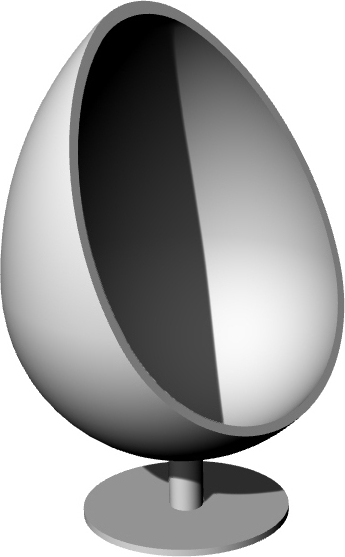
\includegraphics[height=4cm]{fig/case-study-egg-chair}}
  \hfill
  \subcaptionbox{Simple 4-leg chair.\label{fig:eval.studies.designs.thonet214}}
    [.2\linewidth]{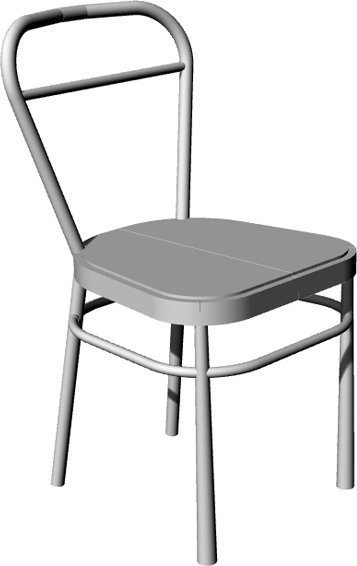
\includegraphics[height=4cm]{fig/case-study-thonet-214}}
  \hfill
  \subcaptionbox{Islamic towers.\label{fig:eval.studies.designs.petronas}}
    [.2\linewidth]{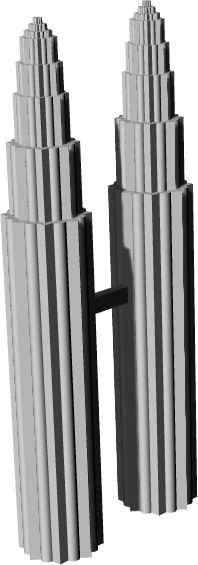
\includegraphics[height=4cm]{fig/case-study-petronas}}
  \hfill
  \subcaptionbox{Voronoi cage.\label{fig:eval.studies.designs.watercube}}
    [.35\linewidth]{%
      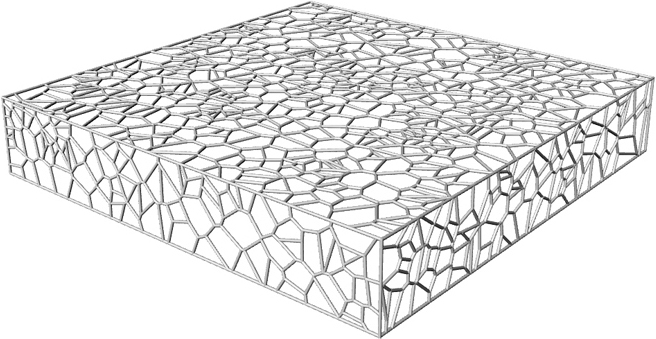
\includegraphics[width=\linewidth]{fig/case-study-water-cube}}
  \caption[Case study design inspirations]{
    Case study designs inspired by the Eero Aarnio's Egg
    chair~\subref{fig:eval.studies.designs.egg}, Thonet 214
    chair~\subref{fig:eval.studies.designs.thonet214},  César Pelli's Petronas
    Twin Towers~\subref{fig:eval.studies.designs.petronas}, and PTW Architects'
    Beijing National Aquatics
    Center~\subref{fig:eval.studies.designs.watercube}.}%
  \label{fig:eval.studies.designs}
\end{figure}

\subsection{Egg}%
\label{sec:eval.studies.egg}

The first case study is an egg shape (which can be considered a particular case
of an oval shape).  Examples of applications of this shape in design include the
Eero Aarnio's Egg chair, James Law's Cybertecture Egg building, and RAU
Architects and Ro\&Ad Architects' Tij observatory.

The egg shape is a broad concept, as it can refer to a wide range of curves
resembling an egg~\cite{Dixon:1991:Mathographics}.  In this case, our shape is
bilaterally symmetric and is composed of four arcs, the side arcs being tangent
to the bottom and top arcs.

Our parametrization of the egg defines four parameters: the bottom arc's center
$O_1$, the bottom and top arcs' radii $r_1$ and $r_2$ respectively, and the
egg's height $h$ (\cref{fig:eval.studies.egg.prob.params}).  Different egg
shapes, more or less elongated, can be obtained by varying the parameters'
values (\cref{fig:eval.studies.egg.prob.vars}).  One of those variations, where
$r_2 = (2 - \sqrt2)r_1$ and $h = 2r_1 + r_2$, corresponds to the Moss' Egg
(\cref{fig:eval.studies.egg.prob}, the egg with $h = 2.6$ and $r_2 = 0.6$).

\begin{figure}[htb]
  \subcaptionbox{\label{fig:eval.studies.egg.prob.params}%
    Egg parametrization: center $O_1$, bottom and top arcs' radii $r_1$ and
    $r_2$, and height $h$.}
    {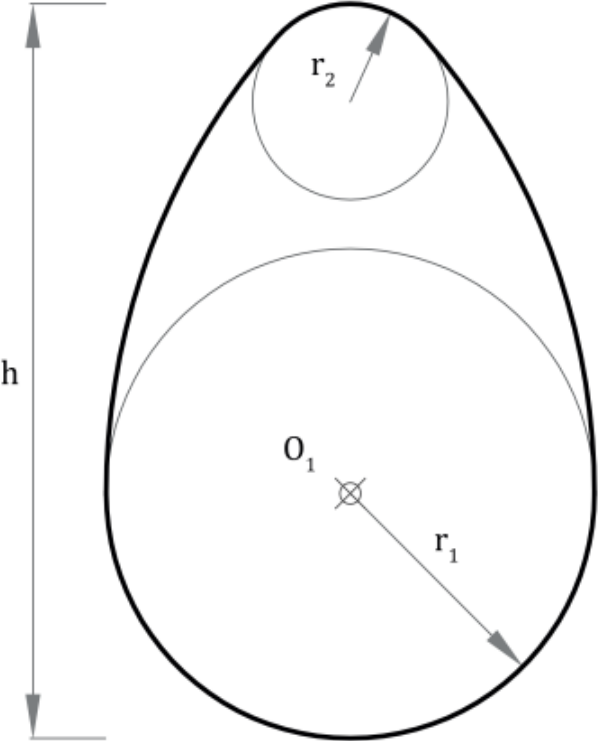
\includegraphics[height=7cm]{fig/egg-problem-params}}
  \hfill
  \subcaptionbox{\label{fig:eval.studies.egg.prob.vars}%
    Egg shape variations: variations change the values of the radius $r_3$ and
    the height $h$.}
    {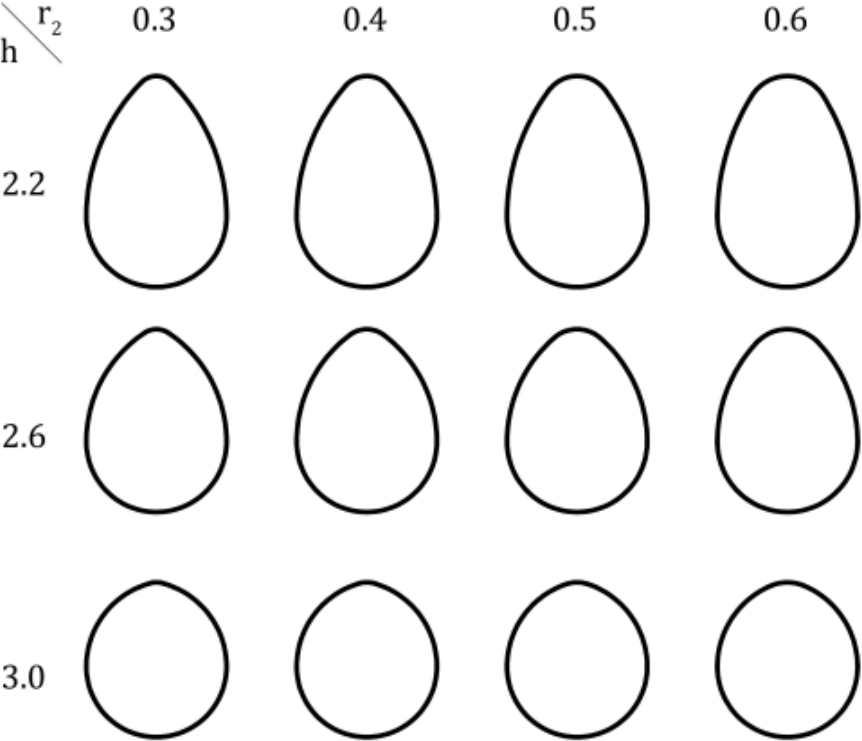
\includegraphics[height=7cm]{fig/egg-problem-vars}}
  \caption[Egg problem]{Egg problem:
  \subref{fig:eval.studies.egg.prob.params} shows our parametrization of the
  egg which can be used to generate shape variations, some of them shown in
  \subref{fig:eval.studies.egg.prob.vars}.}\label{fig:eval.studies.egg.prob}
\end{figure}

In this case, the major problem was to define the side arc $A_3$, which is given
by the center $O_3$, radius $r_3$, and amplitude $\alpha$
(\cref{fig:eval.studies.egg.sol.a}). The \textit{analytic solution} is described
below. The angle $\alpha$ and the radius $r_3$ are devised from the triangle
$\triangle O_1 O_2 O_3$ (\cref{fig:eval.studies.egg.sol.c}), and the center
$O_3$ is given by a translation of $O_1$ through the unit vector $\vec{e}_x$,
parallel to the X-axis, scaled by the factor $r_1 - r_3$.  It is important to
note that, despite their simplicity, the derivations needed to arrive at the
following formulas are not obvious.

\begin{enumerate}
  \item $\alpha = 2\arctan\frac{r_1 - r_2}{h - r_1 - r_2}$
  \item $r_3 = \frac{r_1 - r_2 \cos\alpha}{1 - \cos\alpha}$
  \item $O_3 = O_1 + \left(r_1 - r_2\right)\vec{e}_x$
\end{enumerate}

The \textit{constructive solution} is based on the geometric problem of
determining the \textit{tangent line to two circles}.  In fact, the side arc
$A_3$ is tangent to two circles, $C_1$ and $C_2$, and passes through point
$P_1$.  Two \ac{GC} primitives from our solution were employed in this
solution, namely \textit{intersection} and \textit{bisector}.  The solution can
be computed according to the following procedure
(\cref{fig:eval.studies.egg.sol.c}):

\begin{enumerate}
  \item $C_{2}' = \mathrm{circle}\left(P_1, r_2\right)$%
  \label{enum:eval.studies.egg.cs}
  \item $I = \mathrm{intersection}\left(C_{2}', \overline{O_1 P_2}\right)$
  \item $B = \mathrm{bisector}\left(\overline{IO_2}\right)$
  \item $O_3 = \mathrm{intersection}\left(B, O_1 P_1\right)$
  \item $r_3 = \mathrm{length}\left(\overline{O_3 P_1}\right)$%
  \label{enum:eval.studies.egg.ce}
  \item $\alpha = \mathrm{angle}\left(O_2,O_3,O_1\right)$
\end{enumerate}

We can further increase the expressive level of the solution by defining the
$\mathrm{tangent_{circle}}$ functionality.  Given two circles, $C_1$ and $C_2$,
and a point $P_1$ on $C_1$, $\mathrm{tangent_{circle}}$ produces the circle
tangent to both $C_1$ and $C_2$ that goes through $P_1$.  This way, the solution
can be simplified by replacing steps \ref{enum:eval.studies.egg.cs} through
\ref{enum:eval.studies.egg.ce} by using the $\mathrm{tangent_{circle}}$
functionality as follows:

\begin{enumerate}
  \item $O_3,r_3 = \mathrm{tangent_{circles}}\left(C_1, C_2, P_2\right)$
  \item $\alpha = \mathrm{angle}\left(O_2, O_3, O_1\right)$
\end{enumerate}

In the egg's case, $C_1$ must be larger than $C_2$, and $P_1$ is one of the
intersection points between the horizontal line that passes through $O_1$ and
the circle $C_1$.

\begin{figure}[htb]
  \subcaptionbox{\label{fig:eval.studies.egg.sol.a}%
      Solution using the analytic approach.}
    {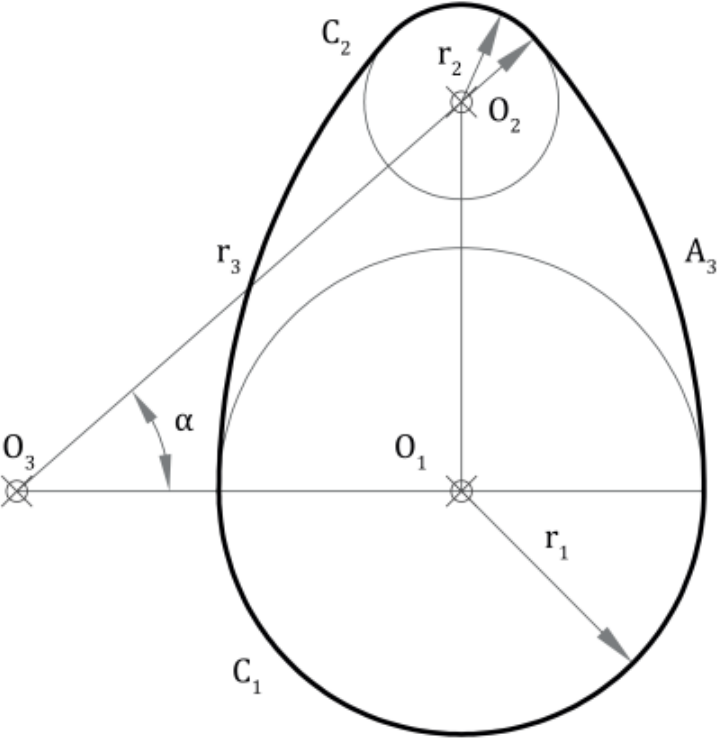
\includegraphics[height=7cm]{fig/egg-solution-analytic}}
  \hspace{\fill}
  \subcaptionbox{\label{fig:eval.studies.egg.sol.c}%
      Solution using the constructive approach.}
    {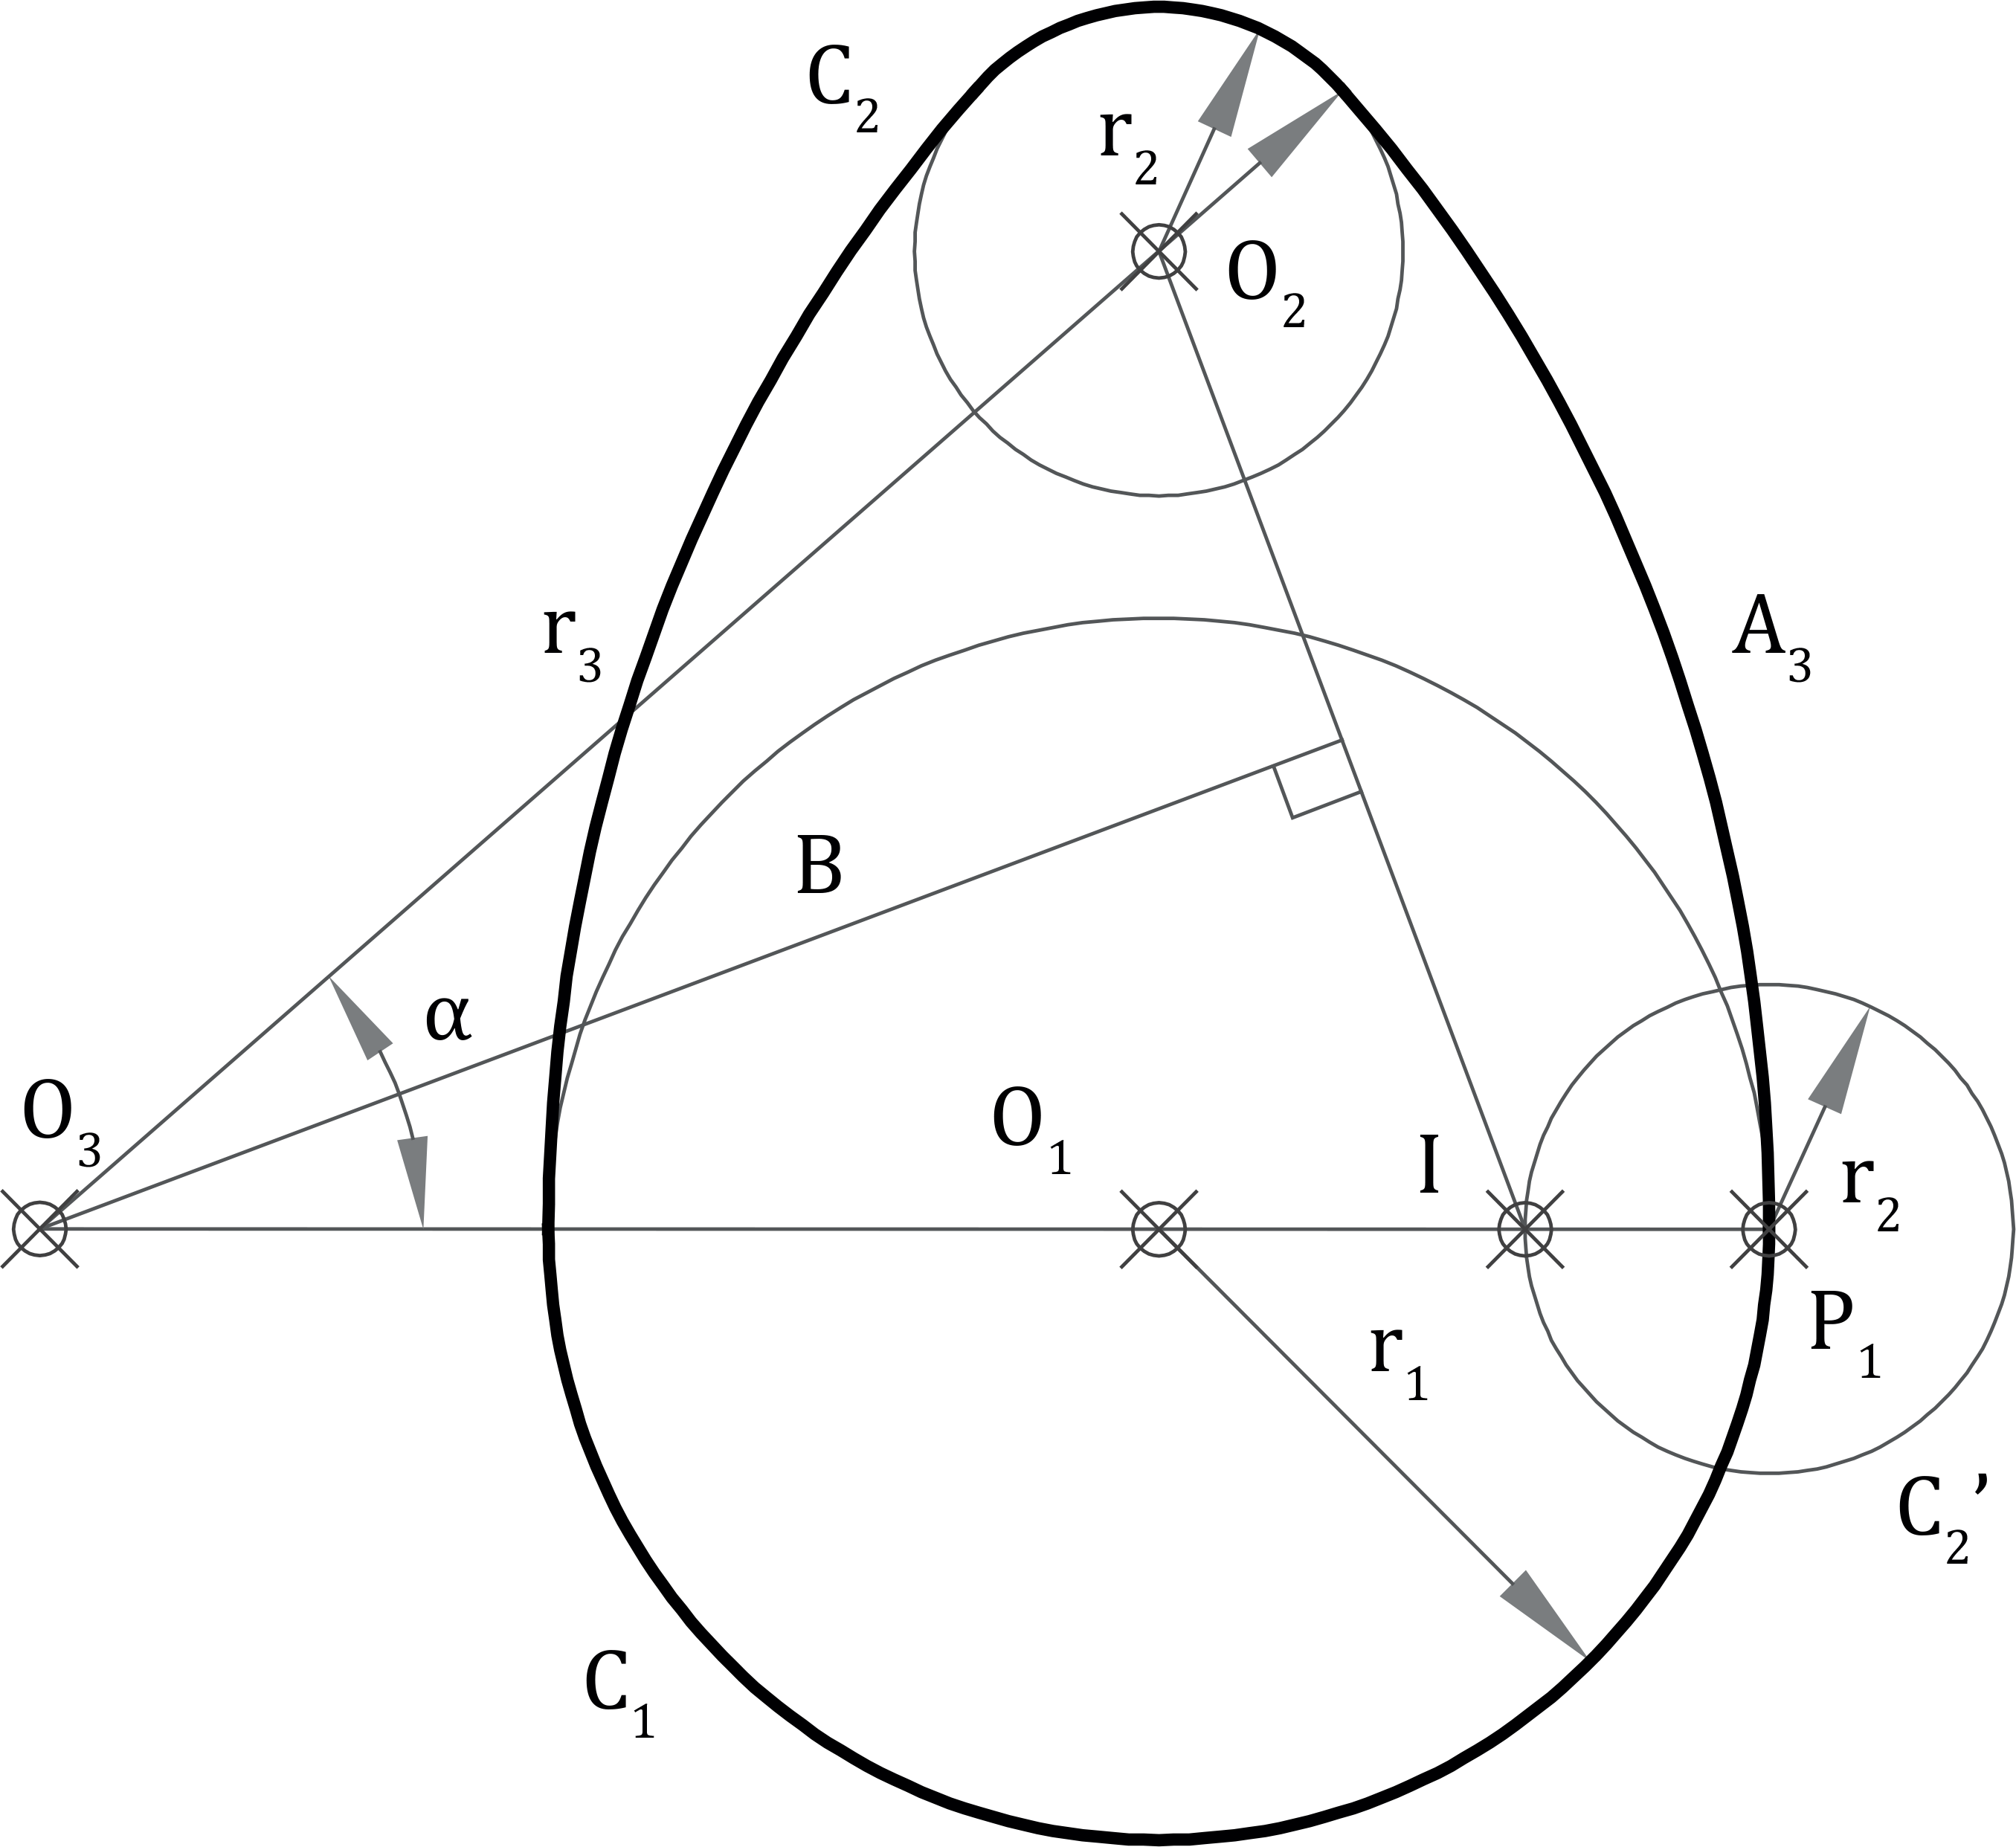
\includegraphics[height=7cm]{fig/egg-solution-constructive}}
  \caption[Egg problem solutions]{Solutions to the Egg problem using two
    different approaches.}%
  \label{fig:eval.studies.egg.sol}
\end{figure}

Achieving the equations in the \textit{analytic solution} is not a
straightforward task for designers, since it involves considerable logical
reasoning and the use of non-trivial formulas (such as trigonometric half-angle
identities). It is also unclear how those equations were derived. By contrast,
in the \textit{constructive solution}, all the steps are clearly externalized,
which makes it much more comprehensible.

\subsection{Rounded Trapezoid}%
\label{sec:eval.studies.rtrapezoid}

The second case study is a rounded trapezoid shape.  This parametric shapes is
used in the contour of a variety of different chair seats, such as the Thonet
214 and the Zig Zag chairs~\cite{Garcia:2018:SGDTIMCG}.  This shape is
bilaterally symmetric and is defined by six parameters: width $w$, depth $d$,
taper width $tw$, front radius $r_f$, rear radius $r_r$, and origin $O$
(\cref{fig:eval.studies.rtrapezoid.prob.params}).  The taper width and front and
rear radii are ratios of the width and the depth.  By varying these parameters'
values, one can obtain different shapes, such as a square, a trapezoid, a
triangle, a rounded rectangle, a drop-like shape, and a circle, among others
(\cref{fig:eval.studies.rtrapezoid.prob.vars}).

\begin{figure}[htb]
  \subcaptionbox{\label{fig:eval.studies.rtrapezoid.prob.params}%
    Trapezoid parametrization: width $w$, depth $d$, taper width $w$, front and
    rear radii $r_f$ and $r_r$ respectively, and origin $O$.}
    {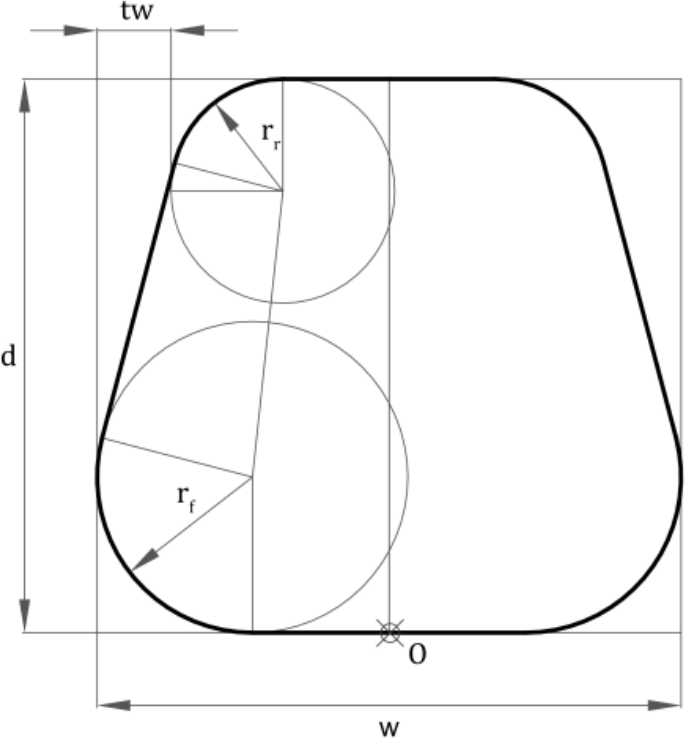
\includegraphics[height=7cm]{fig/rtrapezoid-problem-params}}
  \hfill
  \subcaptionbox{\label{fig:eval.studies.rtrapezoid.prob.vars}%
    Rounded trapezoid shape variations: variations change the values of the
    front radius $r_f$ and the taper width $tw$.}
    {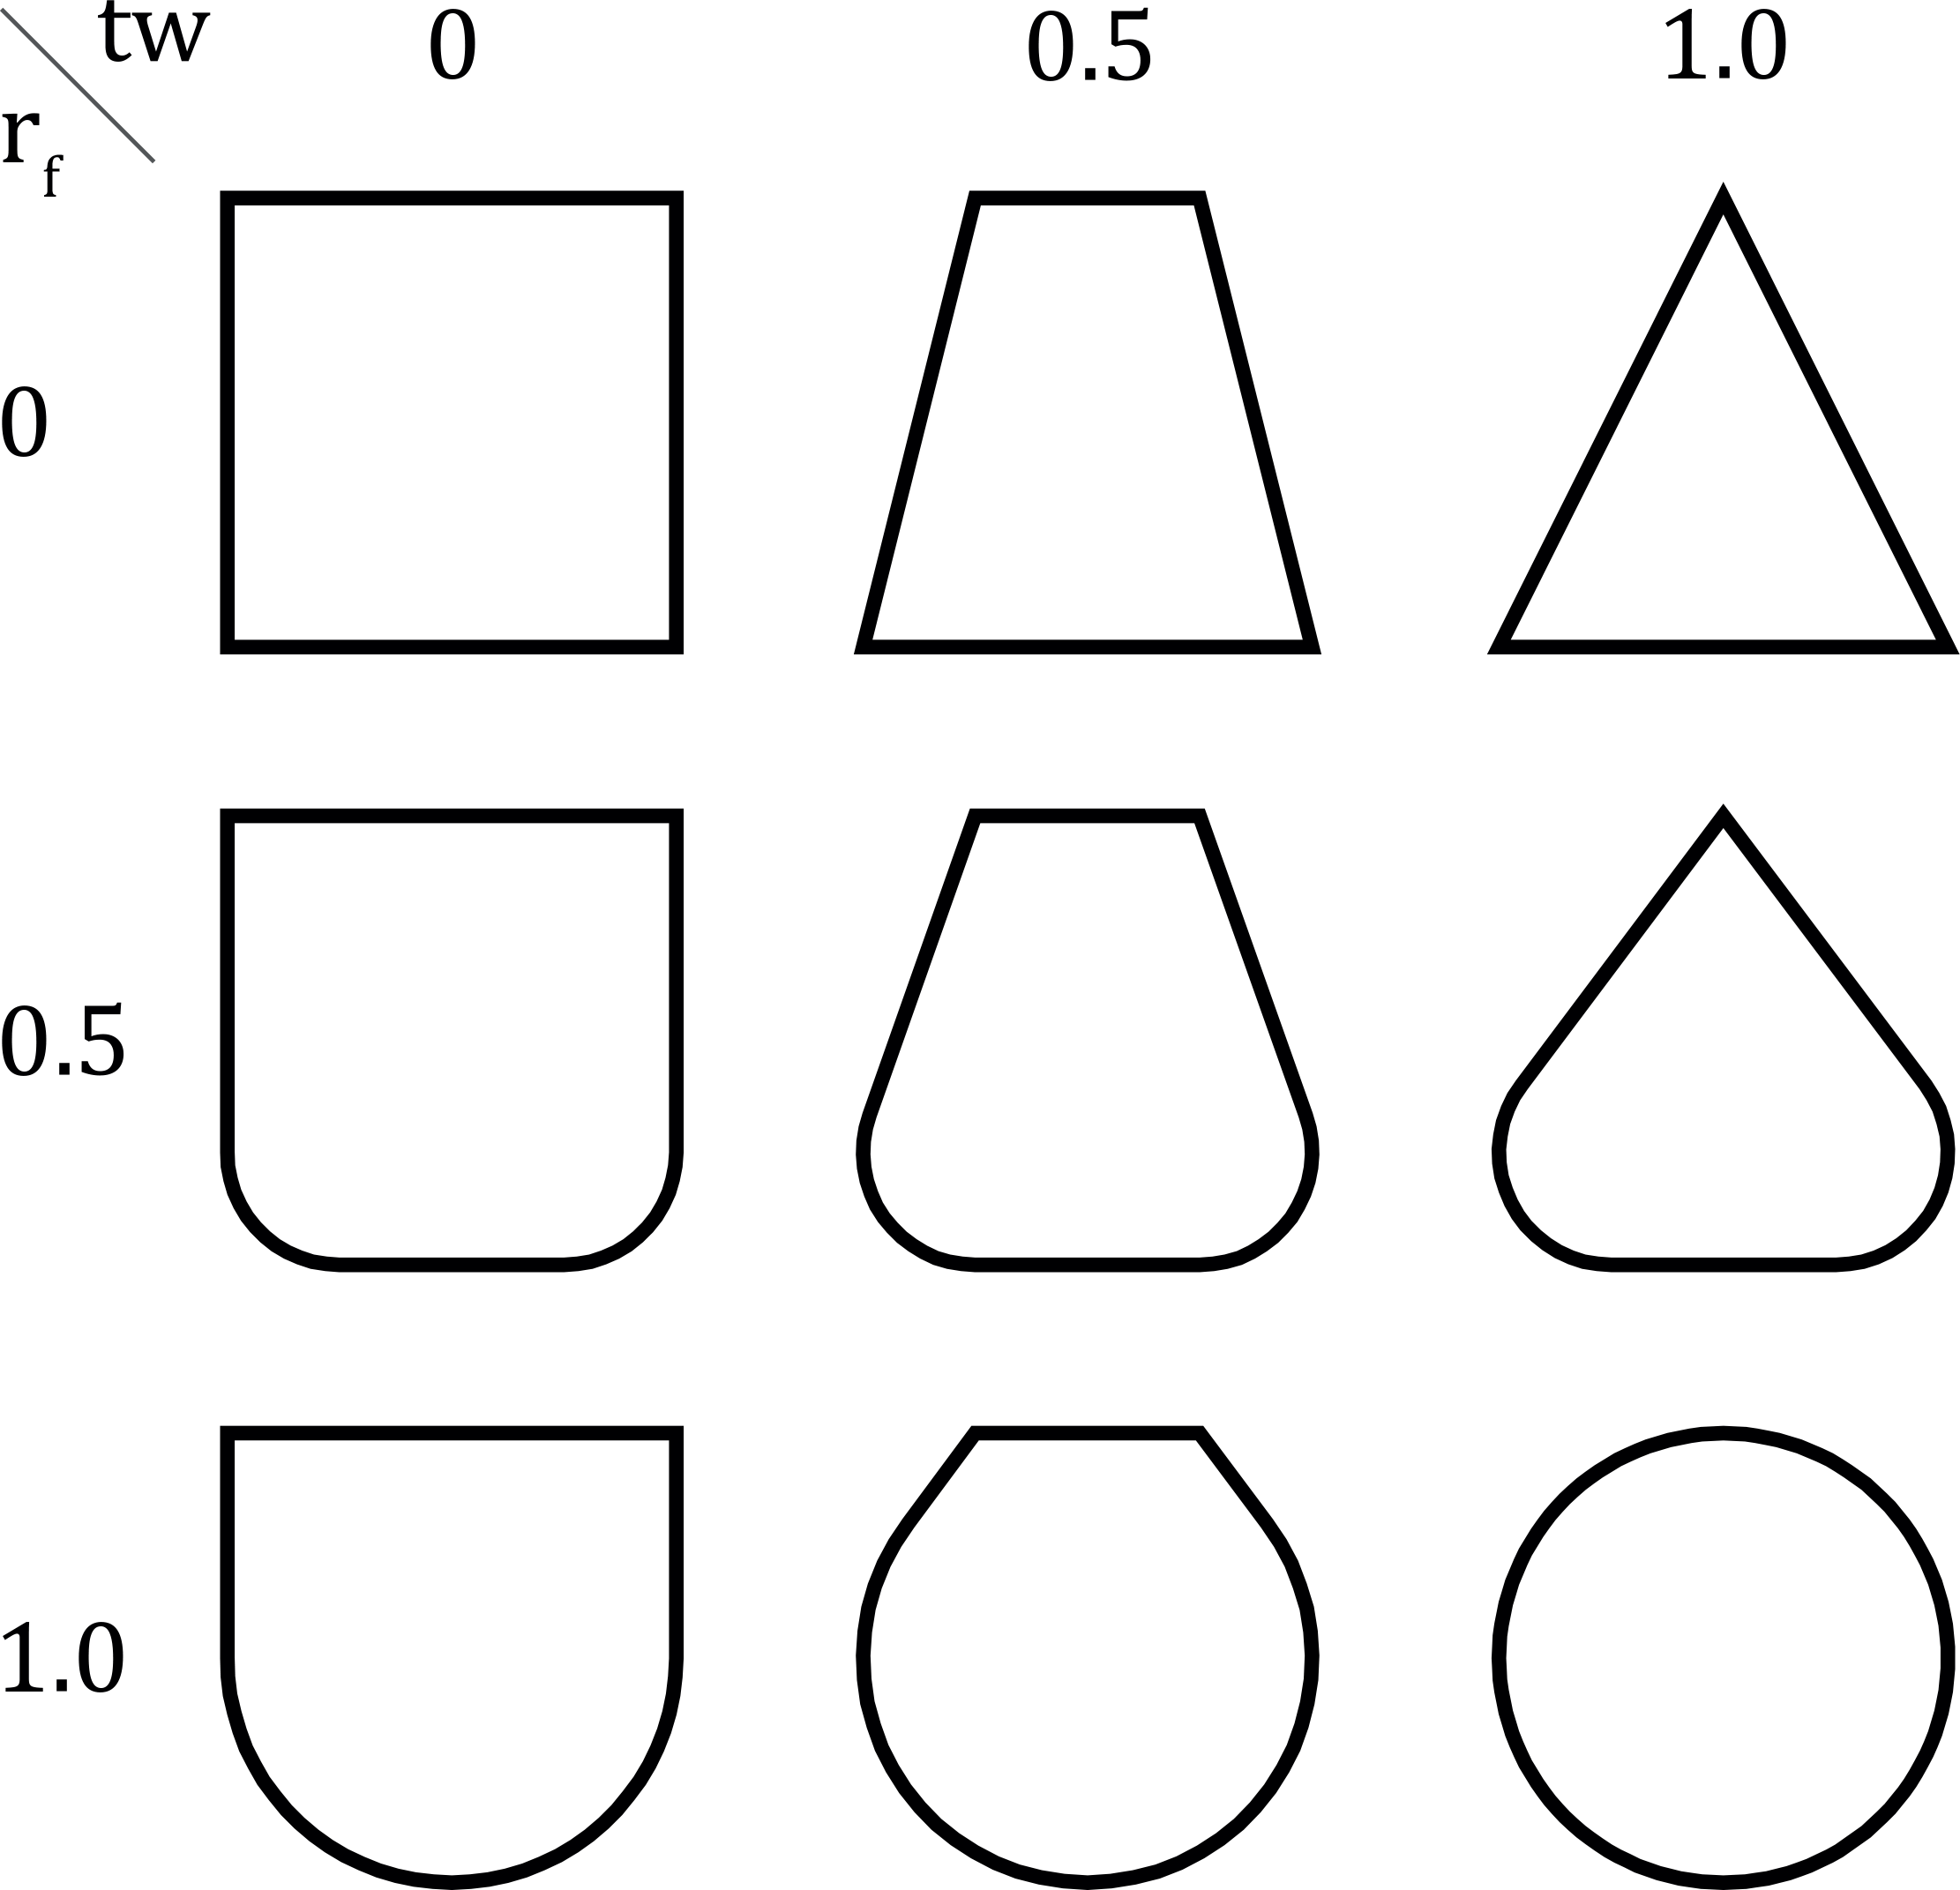
\includegraphics[height=7cm]{fig/rtrapezoid-problem-vars}}
  \caption[Rounded trapezoid problem]{Rounded trapezoid problem:
    \subref{fig:eval.studies.rtrapezoid.prob.params} shows our parametrization
    of the trapezoid which can be used to generate shape variations, some of
    them shown in \subref{fig:eval.studies.rtrapezoid.prob.vars}.}%
  \label{fig:eval.studies.rtrapezoid.prob}
\end{figure}

One side of the chair is obtained by two circles and the \textit{tangent line to
two circles}, while the other side is a reflection of the former side.  Given
two circles $C_2$ and $C_2$, centered on $O_1$ and $O_2$ with radii $r_1$ and
$r_2$ respectively (\cref{fig:eval.studies.rtrapezoid.sol}), two solutions can
be delineated that can accurately reproduce the tangent line $\overline{T_1
T_2}$.

The \textit{analytic solution} is achieved by calculating the angle $\delta$
between the line segment $\overline{O_1 O_2}$ and the line perpendicular to the
tangent line between the two circles passing through $O_1$.  The angle $\theta$
is given by the slope of $\overline{O_1 O_2}$.  The point $T_1$ is given by a
translation of $O_1$ through a vector $\left(r_1, \angle\delta + \theta\right)$
where $r_1$ is its length and $\angle\delta + \theta$ is its polar angle.  A
similar approach is used to obtain $T_2$.

\begin{enumerate}
  \item $\delta = \arccos\frac{r_1 - r_2}{\lVert O_2 - O_1 \rVert}$
  \item $\theta = \angle\vv{O_2 - O_1},\vec{e}_x$
  \item $T_2 = O_1 + \left(r_1, \angle\delta + \theta\right)$
  \item $T_2 = O_2 + \left(r_1, \angle\delta + \theta\right)$
\end{enumerate}

The \textit{constructive solution} follows a sequence of steps that reflects the
geometric characteristics of the problem
(\cref{fig:eval.studies.rtrapezoid.sol}).  Four \ac{GC} primitives were employed
in this solution, namely \textit{midpoint}, \textit{intersection}, and
\textit{parallel lines}.

\begin{figure}
  \centering
  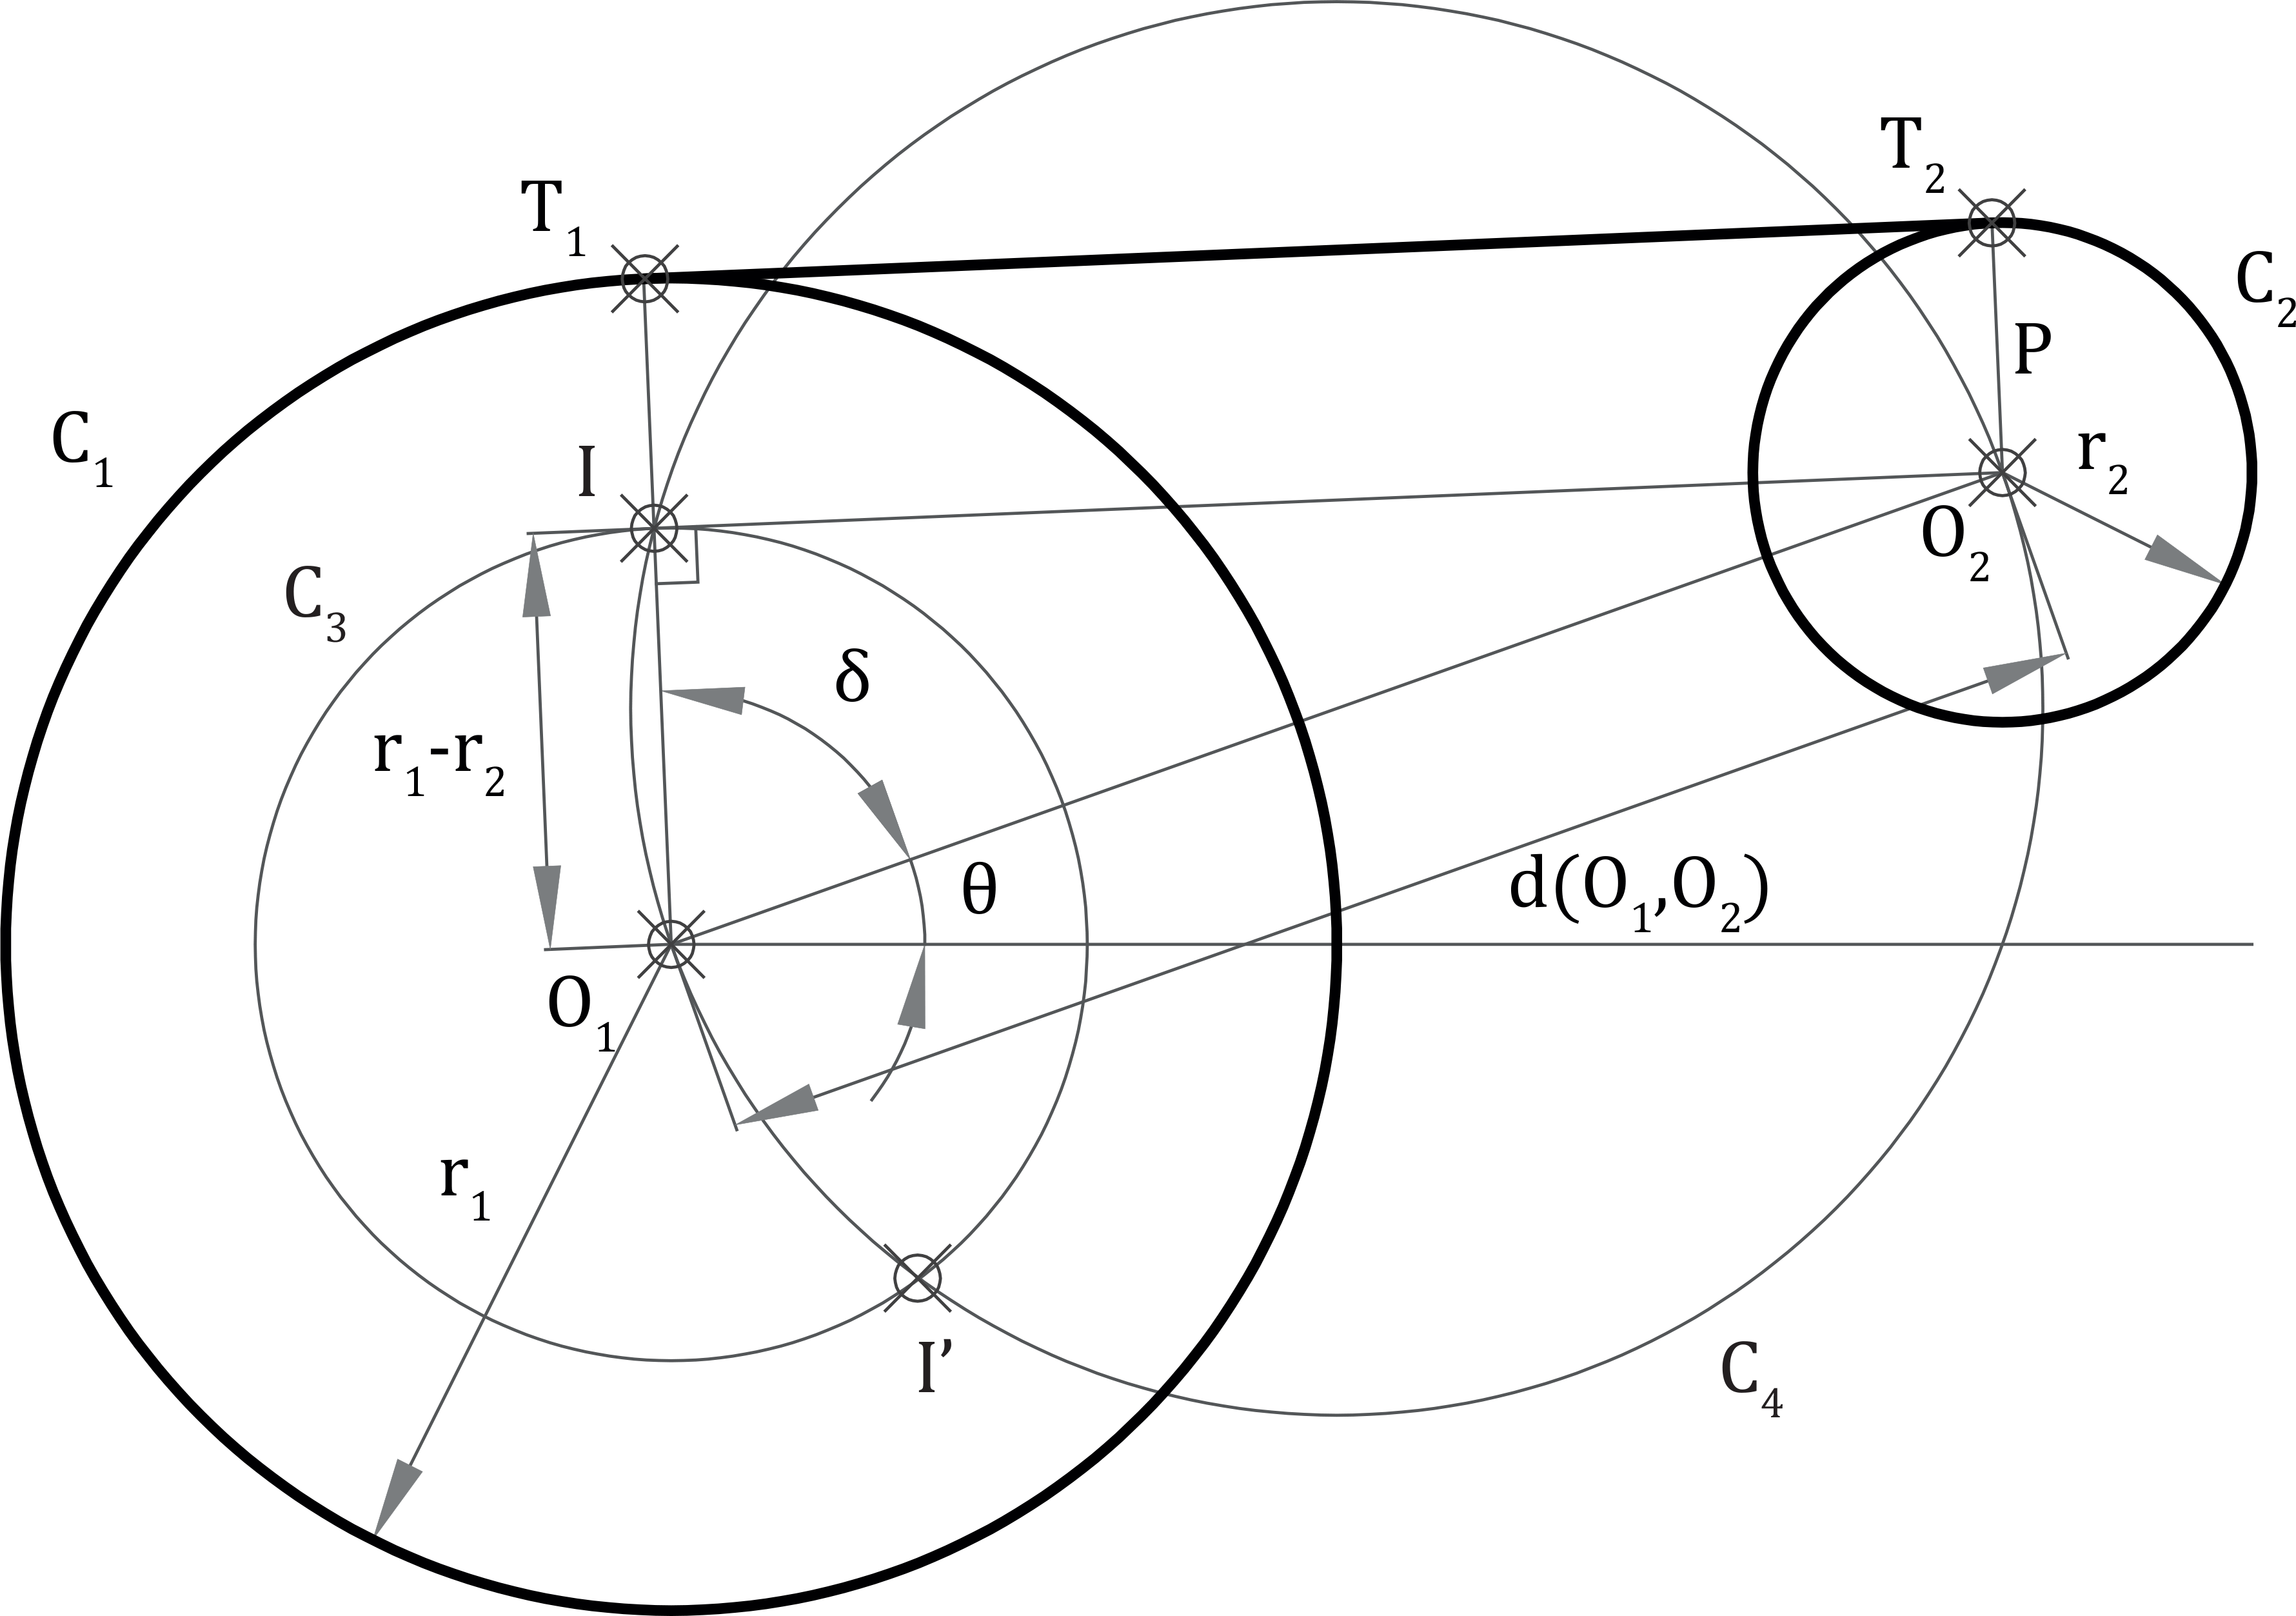
\includegraphics[height=7cm]{fig/rtrapezoid-solution}
  \caption[Rounded trapezoid problem solution]{Both analytic and constructive
    solutions to the rounded trapezoid problem.}%
  \label{fig:eval.studies.rtrapezoid.sol}
\end{figure}

\begin{enumerate}
  \item $C_3 = \mathrm{circle}\left(O_1, r_1 - r_2\right)$
  \item $M = \mathrm{midpoint}\left(O_1, O_2\right)$
  \item $d = \mathrm{length}\left(\overline{O_1 O_2}\right)$
  \item $C_4 = \mathrm{circle}\left(M, \frac{d}{2}\right)$
  \item $I,I' = \mathrm{intersection}\left(C_3, C_4\right)$
  \item $P = \mathrm{parallel}\left(\overline{IO_1, O_2}\right)$
  \item $T_1 = \mathrm{intersection}\left(IO_1, C_1\right)$
  \item $T_2 = \mathrm{intersection}\left(P, C_2\right)$
\end{enumerate}

Despite the adequacy of the \textit{analytic solution} for the design problem at
hand, it only produces the external tangent needed to solve this specific
problem, which works well if the circle's center is on the 1\textsuperscript{st}
and 2\textsuperscript{nd} quadrants: however, in the remaining quadrants, it
produces an unintended tangent.  In contrast, our \textit{constructive approach}
is capable of producing a solution independently of how the circles are
arranged.

The advantage of using well-established functions from \ac{CGAL} is that they
deal with degenerate cases better than re-implementations of the same
functionality from scratch.  For instance, in the case of concentric circles,
the intersection between those circles does not produce an error; instead, it
produces an empty result.  In the case of the proposed \textit{analytic
solution}, the distance between the circles' centers is zero, which leads to a
division-by-zero error.

Architects and designers are used to manipulating \acp{GC}, such as
\textit{tangency}, \textit{parallelism}, and \textit{intersection}, and less
inclined to deal with the mathematical intricacies of analytic geometry, which
makes the second approach more appealing to them.  To that end, we can introduce
the $\mathrm{tangent_{lines}}$ functionality, which, given two circles $C_1$ and
$C_2$, produces a sequence of tangent lines between the circles, allowing the
user to select the lines that best suit the problem.  This allows us to reduce
the solution to the single step
\begin{itemize}
  \item[] $\overline{T_1 T_2},\ldots = \mathrm{tangent_{lines}}\left(C_1,
  C_2\right)$
\end{itemize}
where $\overline{T_1 T_2}$ is one of the lines of the sequence.

Depending on how the circles are arranged, there can be multiple solutions:
\begin{enumerate*}[label= (\arabic*)]
  \item no segments, if one circle contains the other,
  \item two segments, if the circles intersect, or
  \item four segments, if the circles are disjoint.
\end{enumerate*}
The advantage of having the $\mathrm{tangent_{lines}}$ functionality is that it
is capable of finding every solution to the generic \textit{tangent line to two
circles} problem.  Hence, the user can reutilize this functionality each time
a different problem of a similar nature arises.

\subsection{Star with Semicircles}%
\label{sec:eval.studies.star}

The third case study is a star shape with semicircles.  This shape was inspired
by César Pelli's Petronas tower floor plan, which in turn mimics Islamic
patterns.  The contour of the Petronas tower floor plan is formed by two
overlapping congruent squares, forming an octagram known as Star of Lakshmi, and
by eight circles centered on each of the eight intersection points and tangent
to the bounding octagon.  This shape can be generalized to a parametric shape
defined by three parameters: origin $O$, radius $r$, and number of vertices $n$
(\cref{fig:eval.studies.star.prob.params}).  Note that the number of vertices
cannot be less than five.  Five variations, comprising stars with 5 to 9
vertices, are illustrated in \cref{fig:eval.studies.star.prob}.

\begin{figure}[htb]
  \centering
  \subcaptionbox{\label{fig:eval.studies.star.prob.params}%
    Star parametrization: origin $O$, radius $r$, and number of vertices $n$.}
    {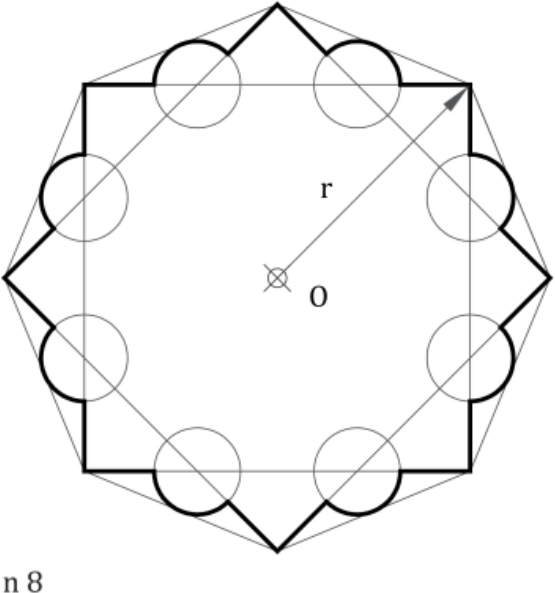
\includegraphics[height=7cm]{fig/star-problem-params}}
  \hfill
  \subcaptionbox{\label{fig:eval.studies.star.prob.vars}%
    Star shape variations: variations change the values of the number of
    vertices $n$.}
    {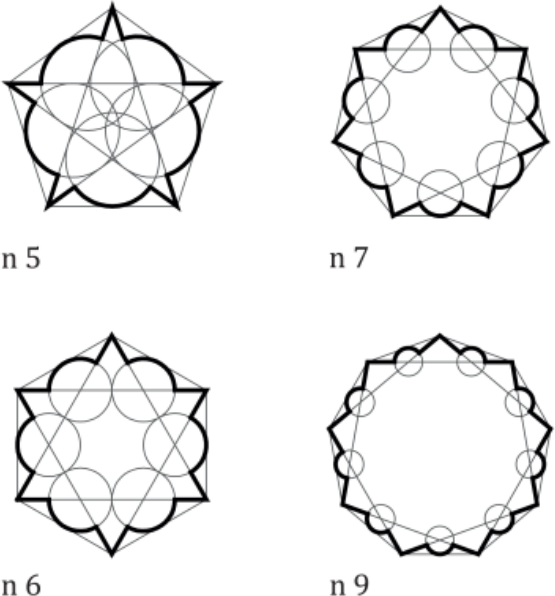
\includegraphics[height=7cm]{fig/star-problem-vars}}
  \caption[Star with semicircles problem]{Star with semicircles problem:
    \subref{fig:eval.studies.star.prob.params} shows our parametrization of
    the star which can be used to generate shape variations, some of them
    shown in \subref{fig:eval.studies.star.prob.vars}.}%
  \label{fig:eval.studies.star.prob}
\end{figure}

Both analytic and constructive solutions are based on computing one side of the
star, composed of the line segment $\overline{V_1 I_1}$, the arc centered on
$O_1$ from $I_1$ to $I_2$, with radius $r_1$, and the line segment 
$\overline{I_2 V_2}$ (\cref{fig:eval.studies.star.sol}).  The remaining sides
result from the recursive application of the preceding side with a rotation
transformation around the center.

\begin{figure}[htb]
  \centering
  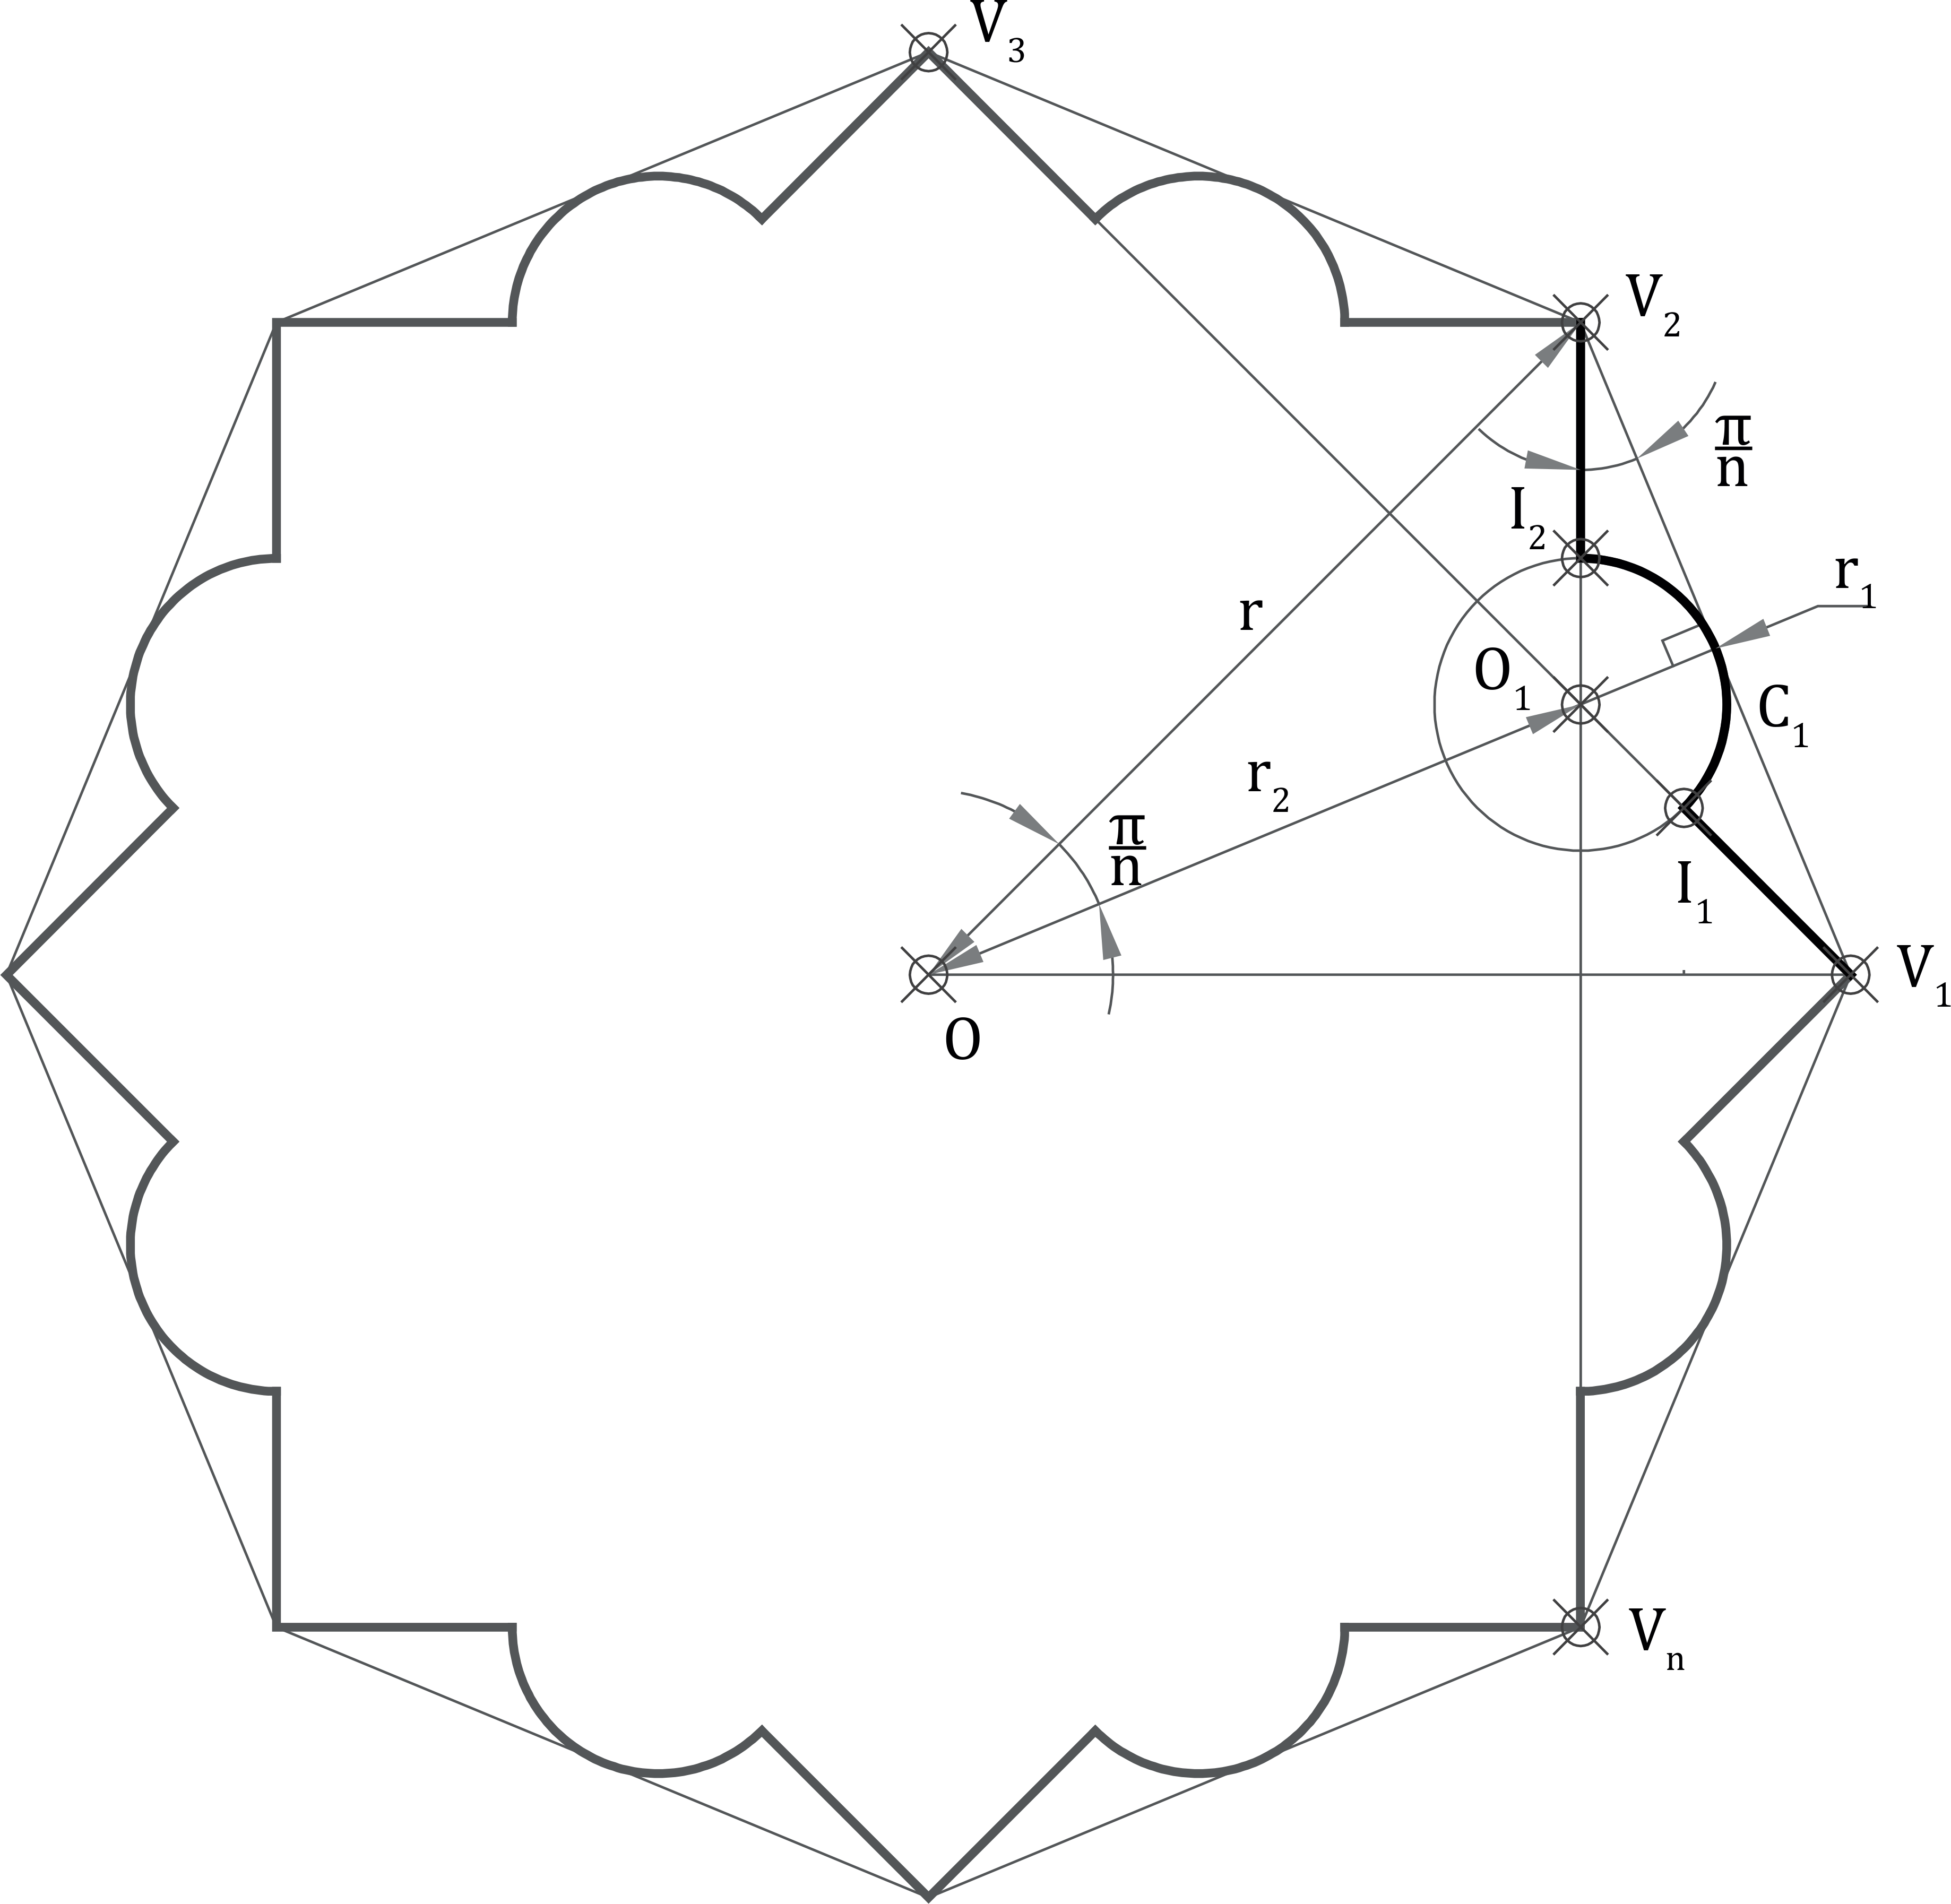
\includegraphics[height=9cm]{fig/star-solution}
  \caption[Star with semicircles problem solution]{ Both analytic and
    construction solutions to the star with semicircles problem.}%
  \label{fig:eval.studies.star.sol}
\end{figure}

The \textit{analytic solution} is described below.  The radius $r_1$ of the
circle $C_1$ is calculated by step \ref{enum:eval.studies.star.r1}, the radius
$r_2$ is defined by step \ref{enum:eval.studies.star.r2}, and its center $O_1$
is given by step \ref{enum:eval.studies.star.O1}.  The intersection points $I_1$
and $I_2$ are given by a rotation around $O_1$
(\cref{fig:eval.studies.star.sol}).

\begin{enumerate}
  \item $r_1 = r\frac{\sin^2\frac{\pi}{n}}{\cos\frac{\pi}{n}}$%
  \label{enum:eval.studies.star.r1}
  \item $r_2 = r\cos\frac{\pi}{n} - r_1$%
  \label{enum:eval.studies.star.r2}
  \item $O_1 = O + \left(r_2, \angle\frac{\pi}{n}\right)$%
  \label{enum:eval.studies.star.O1}
  \item $I_1 = O_1 + \left(r_1, \angle\frac{2\pi}{n} - \frac{\pi}{2}\right)$
  \item $I_2 = O_1 + \left(r_1, \angle\frac{\pi}{2}\right)$
\end{enumerate}

The \textit{construction solution} is based on finding the position and size of
the circle $C_1$ (see \cref{fig:eval.studies.star.sol}).  Two \ac{GC}
primitives were employed in this solution, namely \textit{intersection}, and
\textit{tangent circle to one line}.

\begin{enumerate}
  \item $O_1 = \mathrm{intersection}\left(\overline{V_1 V_3}, \overline{V_2
  V_n}\right)$
  \item $C_1 = \mathrm{tangent_{circle}}\left(O_1, \overline{V_1 V_2}\right)$
  \item $P,r_1 = C_1$
  \item $I_1 = \mathrm{intersection}\left(\overline{V_1 V_3}, C_1\right)$
  \item $I_2 = \mathrm{intersection}\left(\overline{V_2 V_n}, C_1\right)$
\end{enumerate}

As seen in the other cases, the constructive solution is more understandable, as
one can easily reproduce it step-by-step by hand, using a ruler and a compass.

\subsection{Voronoi Diagram}%
\label{sec:eval.studies.voronoi}

Our fourth case study is that of Voronoi diagrams, which are used in a variety
of design fields.  For instance, several facade designs exhibit a Voronoi
appearance, such as PTW Architects' Beijing National Aquatics Center,
ARM\footnote{\url{https://armarchitecture.com.au/projects/melbourne-recital-centre/}.
Not to be mistaken with the ARM family of computing architectures for computer
processors.} Architecture's Melbourne Recital Centre, and Hassell's Alibaba
Headquarters.

In its simplest version, a Voronoi diagram consists of partitioning a plane into
regions from a set of points, called \textit{sites}; for every site, each region
contains every point in the plane closer to that site than to any other site.
The sites are typically randomly distributed points, although they can follow
other distributions.  \Cref{fig:eval.studies.voronoi.prob} shows three Voronoi
diagrams generated from entirely randomly distributed points
(\cref{fig:eval.studies.voronoi.prob.rand}), from random points with one
attractor point in the bottom-left corner
(\cref{fig:eval.studies.voronoi.prob.1attr}), and from random points with one
attractor line at the bottom edge (\cref{fig:eval.studies.voronoi.prob.edge}).
An attractor object is responsible for controlling the density of random points
based on the distance to it.

\begin{figure}[htb]
  \subcaptionbox{\label{fig:eval.studies.voronoi.prob.rand}%
    Randomly distributed points.}
    {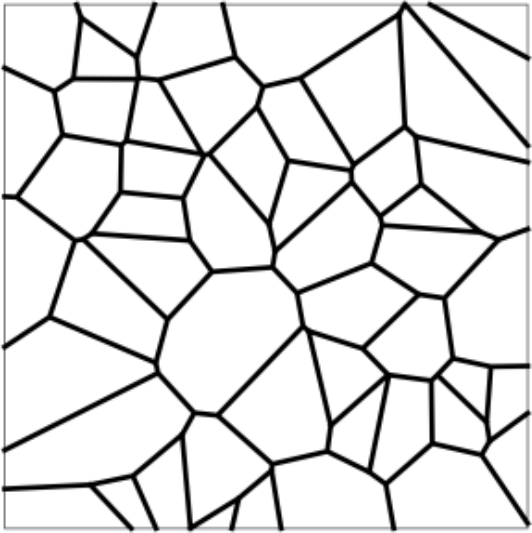
\includegraphics[height=5cm]{fig/voronoi-problem-rand}}
  \hfill
  \subcaptionbox{\label{fig:eval.studies.voronoi.prob.1attr}%
    Randomly distributed points with one attractor point in the bottom-left.}
    {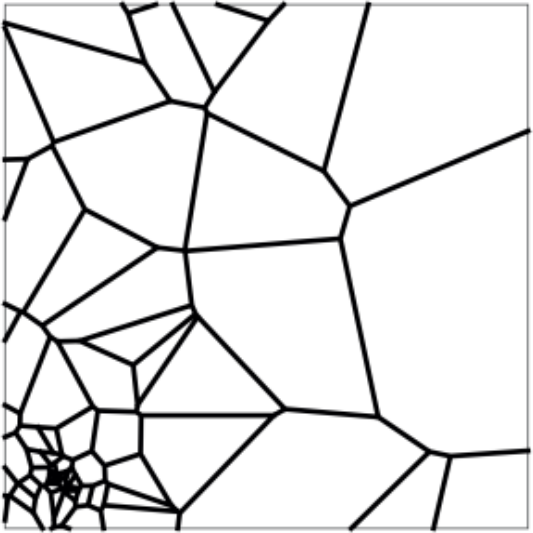
\includegraphics[height=5cm]{fig/voronoi-problem-1attr}}
  \hfill
  \subcaptionbox{\label{fig:eval.studies.voronoi.prob.edge}%
    Randomly distributed points with an attractor line at the bottom.}
    {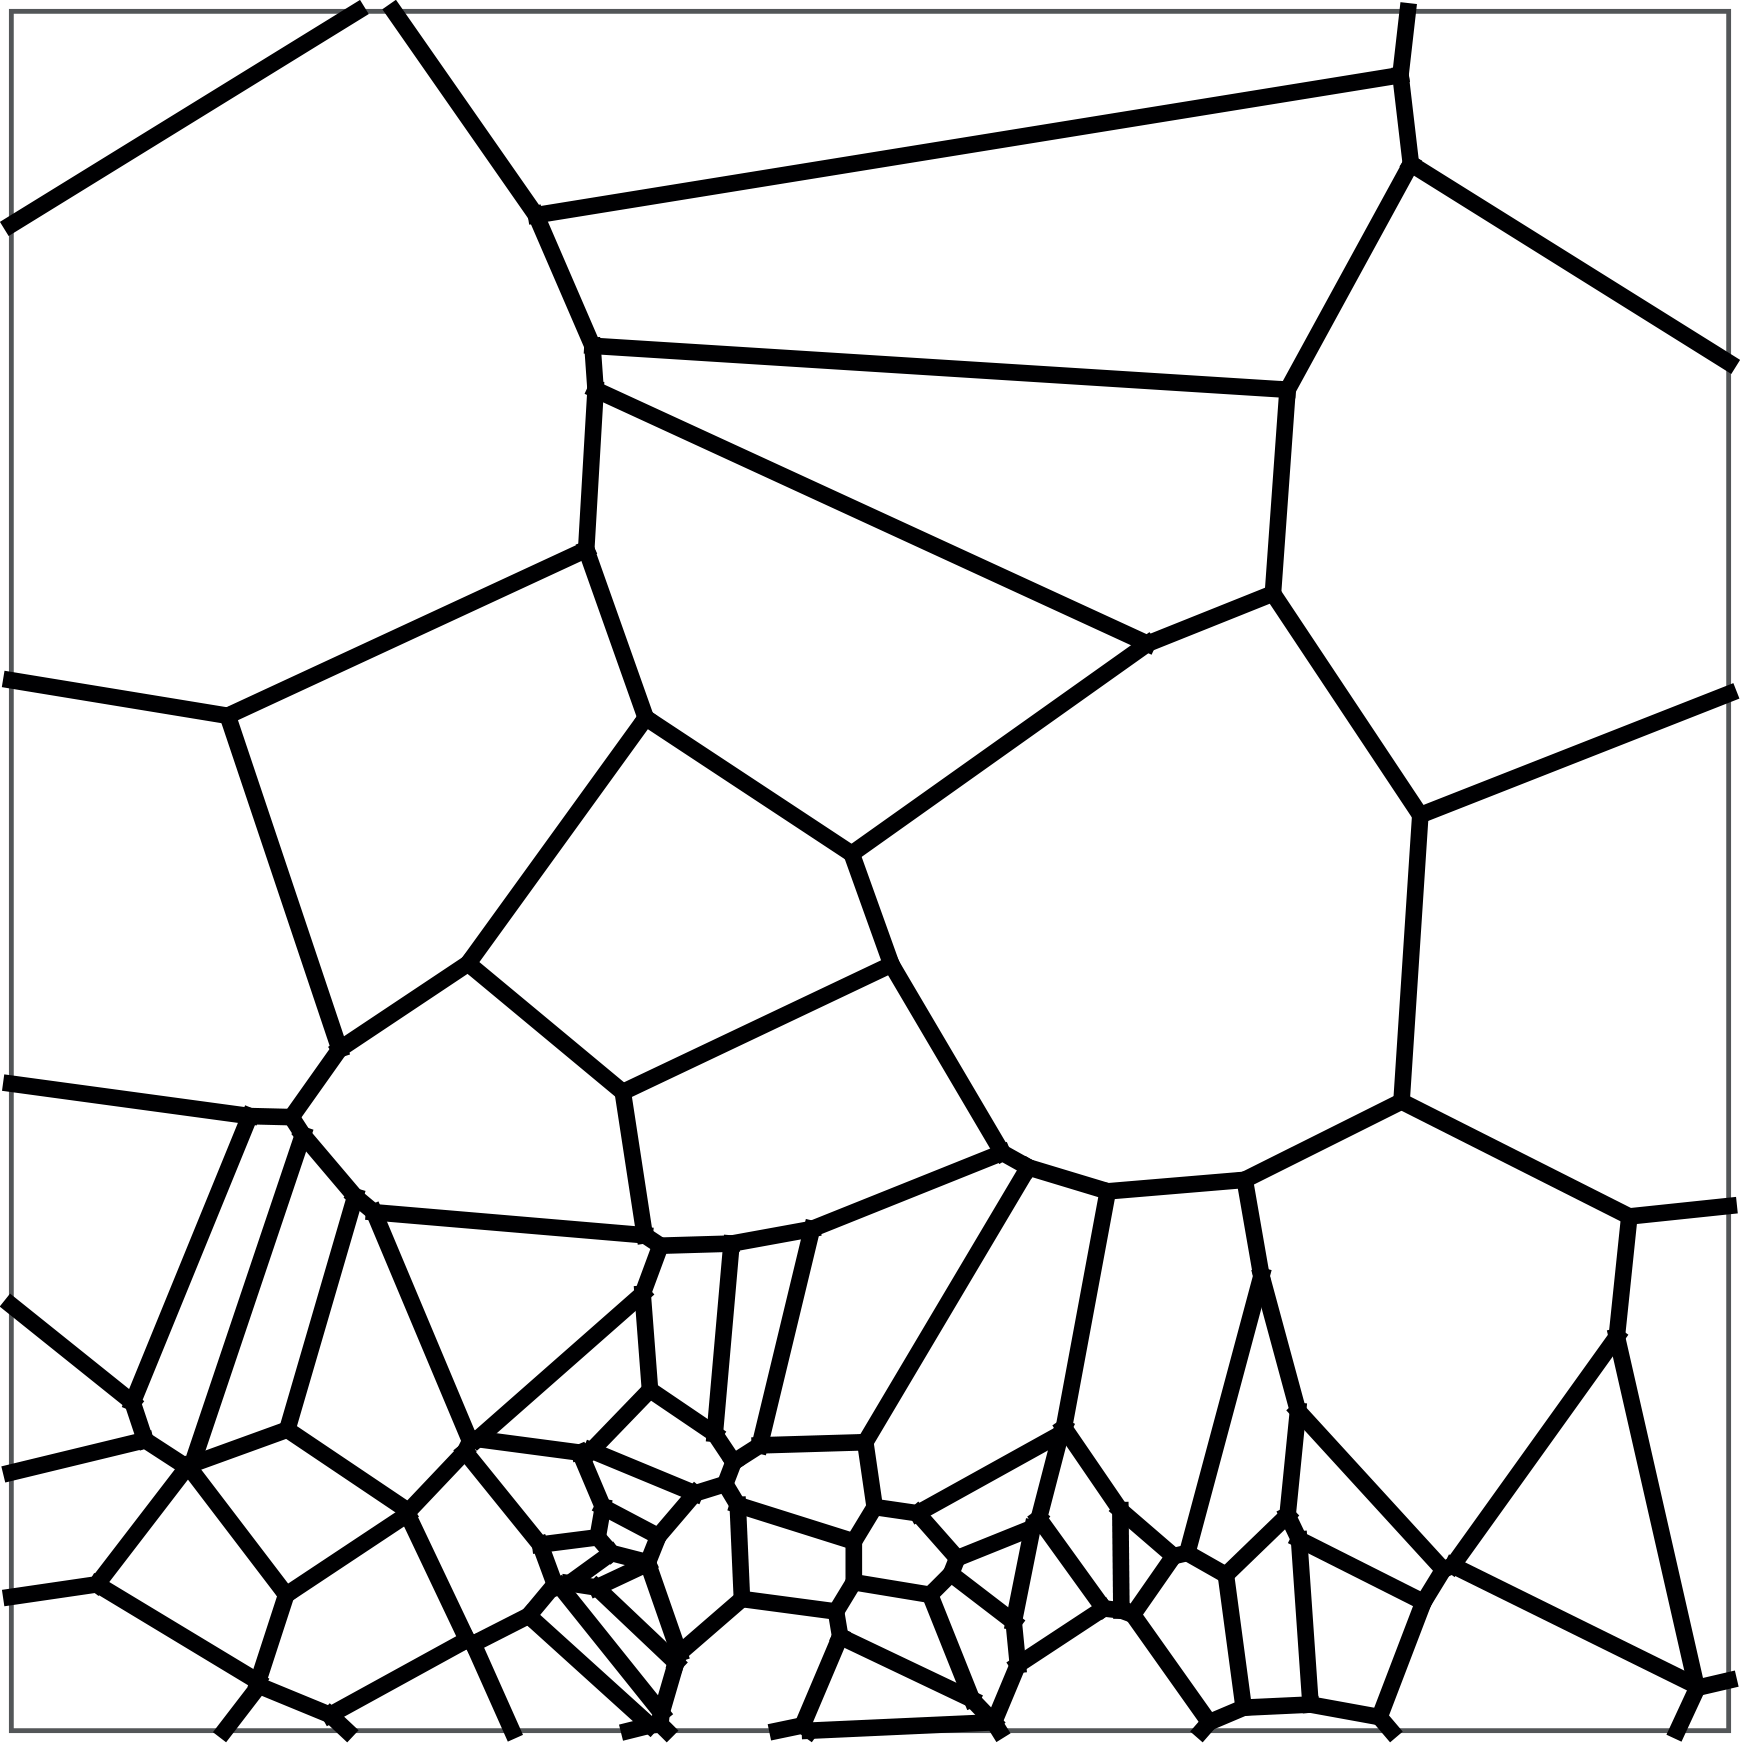
\includegraphics[height=5cm]{fig/voronoi-problem-edge}}
  \caption[Voronoi diagram problem]{
    Voronoi diagram problem: depicted are three Voronoi diagrams variations
    which are mostly generated at random.
    \subref{fig:eval.studies.voronoi.prob.rand} is entirely random,
    \subref{fig:eval.studies.voronoi.prob.1attr} expands on the latter with an
    attractor point, and \subref{fig:eval.studies.voronoi.prob.edge} goes even
    further by using an entire attractor line.}%
  \label{fig:eval.studies.voronoi.prob}
\end{figure}

Both the analytic and constructive methods focus on computation of a vertex
relies on the computation of the \textit{circumcenter} of a triangle, for
instance, triangle $\triangle P_1 P_2 P_3$
(\cref{fig:eval.studies.voronoi.sol}).

\begin{figure}[htb]
  \centering
  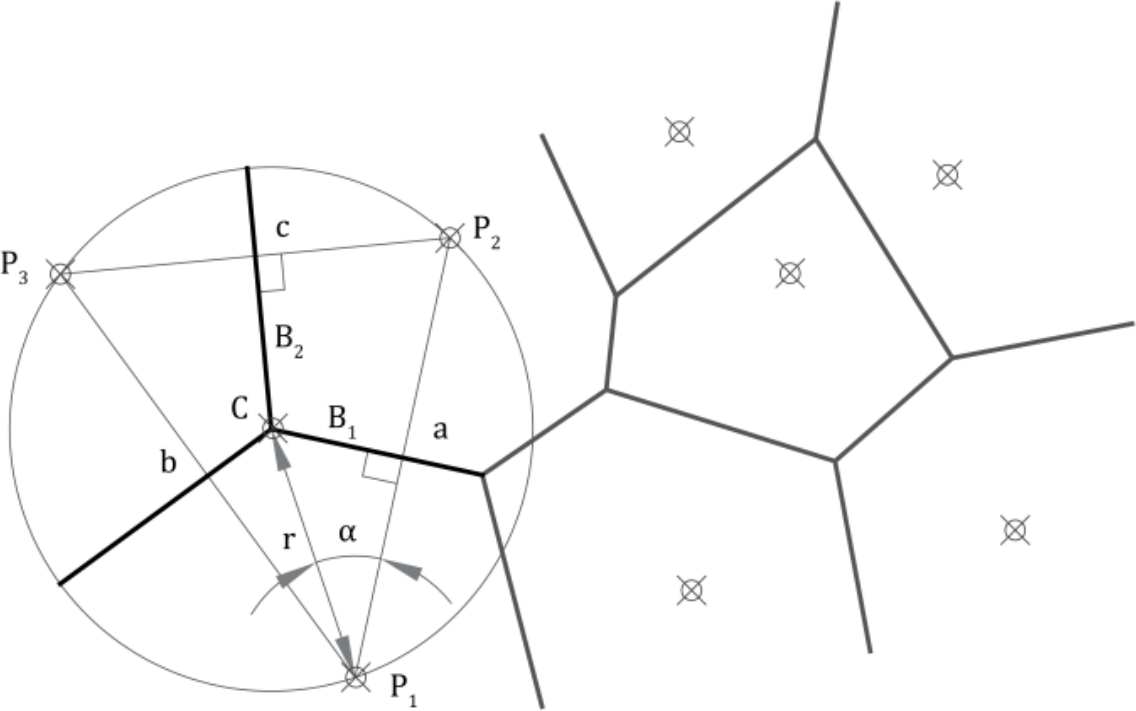
\includegraphics[height=6cm]{fig/voronoi-solution}
  \caption[Voronoi problem partial solution]{
    Analytic and constructive approaches to computing a Voronoi vertex via
    computing the circumcenter of every triangle in the Delaunay triangulation
    whose vertices are the Voronoi diagram's sites.}%
  \label{fig:eval.studies.voronoi.sol}
\end{figure}

There are several possible \textit{analytic solution} to compute a triangle's
circumcenter.  One of them is based on the \textit{circumradius} formula (step
\ref{enum:eval.studies.voronoi.sol.a.circum}), where $a$, $b$, and $c$ are the
lengths of the triangle's sides (step
\ref{enum:eval.studies.voronoi.sol.a.tri}) and $A$ is the triangle's area (step
\ref{enum:eval.studies.voronoi.sol.a.area}).  The circumcenter $C$ can then be
easily computed by a translation (step
\ref{enum:eval.studies.voronoi.sol.a.move}) from $P_1$ following the angle
$\alpha$ (step \ref{enum:eval.studies.voronoi.sol.a.alpha}).

\begin{enumerate}
  \item $a, b, c = \lVert P_2 - P_1 \rVert, \lVert P_3 - P_1 \rVert, \lVert P_3
  - P_2 \rVert$%
  \label{enum:eval.studies.voronoi.sol.a.tri}
  \item $s = \frac{a + b + c}{2}$
  \item $A = \sqrt{s(s - a)(s - b)(s - c)}$%
  \label{enum:eval.studies.voronoi.sol.a.area}
  \item $r = \frac{abc}{4A}$%
  \label{enum:eval.studies.voronoi.sol.a.circum}
  \item $\alpha = \arccos\frac{a}{2r}$%
  \label{enum:eval.studies.voronoi.sol.a.alpha}
  \item $C = P_1 + \left(r, \angle\alpha\right)$%
  \label{enum:eval.studies.voronoi.sol.a.move}
\end{enumerate}

The \textit{constructive solution} computes the circumcenter, given by the
intersection of the edges' perpendicular bisectors.  In fact, this has been
exemplified in \cref{chap:intro}.  Two \ac{GC} primitives were employed in this
solution, namely \textit{bisector} and \textit{intersection}.

\begin{enumerate}
  \item $B_1 = \mathrm{bisector}\left(\overline{P_1 P_2}\right)$
  \item $B_2 = \mathrm{bisector}\left(\overline{P_2 P_3}\right)$
  \item $C = \mathrm{intersection}\left(B_1, B_2\right)$
\end{enumerate}

We can increase the abstraction level of the solution by using the
\textit{circumcenter} functionality implemented in our solution, which, in
reality, is implemented in \ac{CGAL}:

\begin{enumerate}
  \item $C = \mathrm{circumcenter}\left(P_1, P_2, P_3\right)$
\end{enumerate}

The circumcenter problem is only a small part of the generation of a Voronoi
diagram, since we first need to build a Delaunay triangulation.  We can then 
apply the $\mathrm{circumcenter}$ functionality to find the Voronoi vertices and
draw the diagram's edges.  This set of steps can be abstracted away in a
functionality called \textit{voronoi} that, given a set of points $P_S$,
produces a 2D Euclidean Voronoi diagram:

\begin{enumerate}
  \item $V = \mathrm{voronoi}\left(P_S\right)$
\end{enumerate}

Implementing this functionality from scratch is a demanding and error-prone
task.  Fortunately, \ac{CGAL} already has an algorithm that produces robust 2D
Euclidean Voronoi diagrams that can handle degenerate cases, such as dealing
with three or more collinear points.  This algorithm, much like the
\textit{circumcenter} functionality, was entirely repurposed, and made available
in \texttt{CGAL.jl}, and, thus, it is also available in our solution.

% !TeX root = ../../main.tex
\section{Voronoi Diagrams Extended}%
\label{sec:eval.voronoi}

In the previous section, we left the problem of Voronoi Diagrams partially
unresolved, only tackling a small sub-problem required for computing the
diagram's vertices.  This section expands on it by showing how we can repurpose
\ac{CGAL}'s version of the Voronoi Diagram algorithm~\cite{CGAL:5.3:VDA2} as a
beneficial side effect of integrating with the library.  Additionally, we
compare said version with a native Julia implementation of the algorithm
described in~\cite{Springel:2010:GCHSMM} available in the
\texttt{VoronoiDelaunay.jl}\footnote{\url{https://github.com/JuliaGeometry/VoronoiDelaunay.jl}}
package.  Measurements involved obtaining an estimate of the effort required to
create either implementation, measuring Delaunay Triangulation construction
performance, and subsequent output triangulation and diagram comparison.

Both implementations adopt a similar incremental approach and are both robust.
The version from \texttt{VoronoiDelaunay.jl}, however, uses floating point
filtering~\cite{Springel:2010:GCHSMM}, requiring all point coordinates to be in
the interval $\left(1, 2\right) \times \left(1, 2\right) \subset \mathbb{R}^2$;
a restriction \ac{CGAL}'s implementation does not have since it uses a dynamic
floating point precision approach\footnote{Briefed at
\url{https://www.cs.cmu.edu/~quake/robust.html}}~\cite{Shewchuk:1997:APFPAFRGP}.
The \textit{limitation} in the former arguably constitutes a minor inconvenience
since the diagram may be produced in that limited range and then scaled
afterwards to meet the use case's needs.  But it is worth noting the issue is
not present in \ac{CGAL}'s implementation.  This is relevant if the input
coordinates cannot be altered to meet those needs.

To illustrate how we obtained the 2D Delaunay Triangulation and Voronoi Diagram
algorithms from \ac{CGAL}, \cref{lst:appendix.voronoi.jlcxx} shows a minimal
working example of the wrapper library code supported by JlCxx required to make
the necessary constructs and functionality available in Julia.  It follows a
familiar approach, the same used to obtain the core constructs supporting our
\primitives{} solution.  \Cref{lst:eval.voronoi.jl} shows a bare-bones Julia
module encapsulating and exposing the mapped functionality to the Julia
language.
\begin{listing}[htb]
  \inputminted{julia}{jl/Voronoi.jl}
  \caption[Bare-bones Julia module wrapping CGAL's Delaunay algorithms]{
    Bare-bones Julia module wrapping \ac{CGAL}'s 2D Delaunay Triangulation and
    Voronoi Diagrams, supported by the JlCxx wrapper in
    \cref{lst:appendix.voronoi.jlcxx}.}%
  \label{lst:eval.voronoi.jl}
\end{listing}
\texttt{CGAL.jl} contains a version of these mappings that are, however,
parameterized, and adds methods for querying, insertion, and further
manipulation.  For the purposes of testing, we used the slimmer \texttt{Voronoi}
module (\cref{lst:eval.voronoi.jl}).

The process for obtaining these bindings is a relatively simple one that
requires bare minimal C++ knowledge and following reference documentation as if
it were a recipe book, looking up the necessary ingredients and adding them to
the mix.  Accounting for trial and error, in case a minute detail was
overlooked, to make this functionality available would take no more than a full
day.  Having that, the algorithms are ready and available for use.

The algorithm present in \texttt{VoronoiDelaunay.jl} is the result of an immense
body of research, detailed in the \textsc{Arepo}
paper~\cite{Springel:2010:GCHSMM}.  Julia is an expressive language that greatly
benefits prototyping.  Changes are easy to apply and test without the overhead
of compilation, a downside of prototyping in C++, especially when compiling
(against) a sizeable codebase.  We can only infer that the development of the
algorithm did not take long to draft.  However, we can certainly say that it
took more than a full day to obtain a robust implementation, far exceeding the
effort taken by just repurposing an existing robust implementation in \ac{CGAL}.
It required interpretation and understanding of the approach described in the
article since there is no explicit algorithm listed.  This then requires the
creation of a conceptual mapping of the algorithm's entities and procedures,
later translating them into corresponding, preferably efficient, data structures
and functions in the Julia language.  These are among other trials and
tribulations that we did not have to meet in the slightest.  Our estimate is
that developing the algorithm in \texttt{VoronoiDelaunay.jl} took far longer
than obtaining one via our approach.

Regarding both algorithms' performance, \cref{tab:eval.voronoi.bench} shows a
series of results obtained by batch inserting various powers-of-ten sets of
points into Delaunay Triangulation objects, effectively building the meshes.
The results are plotted in \cref{fig:eval.voronoi.bench} for a better
understanding of the tabulated results.  The source code used to perform these
tests is listed in \cref{lst:appendix.voronoi.benchjl}.  More detailed data can
be seen in \cref{lst:appendix.voronoi.data}.

\begin{table}[htb]
  \caption[Delaunay Triangulation benchmarks]{
    Execution times for the construction of Delaunay Triangulations, comparing
    implementations of the algorithm: one from \ac{CGAL} and one from
    \texttt{VoronoiDelaunay.jl}.}%
  \label{tab:eval.voronoi.bench}
  \centering
  \begin{tabular}{r*{2}{l}}
    \toprule
    \multirow{2}{*}{\textbf{\# Points}}
    & \multicolumn{2}{c}{\textbf{Execution time (mean ± σ)}} \\
    & \multicolumn{1}{c}{\texttt{Voronoi.jl}}
    & \multicolumn{1}{c}{\texttt{VoronoiDelaunay.jl}} \\
    \midrule
    10\textsuperscript{2} & \verb| 42.145 μs ±  5.638 μs|
                          & \verb| 53.799 μs ±  39.811 μs| \\
    10\textsuperscript{3} & \verb|509.757 μs ±  1.258 ms|
                          & \verb|510.851 μs ± 113.523 μs| \\
    10\textsuperscript{4} & \verb|  5.879 ms ±  3.874 ms|
                          & \verb|  5.606 ms ± 382.603 μs| \\
    10\textsuperscript{5} & \verb| 62.344 ms ± 11.980 ms|
                          & \verb| 65.103 ms ±   2.287 ms| \\
    10\textsuperscript{6} & \verb|668.331 ms ± 44.458 ms|
                          & \verb|841.925 ms ±  51.394 ms| \\
    \bottomrule
  \end{tabular}
\end{table}

\begin{figure}[htb]
  \centering
  \begin{tikzpicture}
  \begin{loglogaxis}[ybar=0pt,
    title={\texttt{Voronoi.jl} vs.\ \texttt{VoronoiDelaunay.jl}},
    xlabel={Number of Points (log)},
    ylabel={Average Time (ns, log)},
    width={\linewidth},
    height=6cm,
    bar width=3.16227766,% 10^(1/n) where n = 2 (bars)
    enlarge y limits={.2,upper},
    enlarge x limits={abs=3.16227766},
    legend columns=-1,
    table/col sep=comma,
    error bars/y explicit,
    error bars/y dir=both
  ]
    \addplot+ table [y error index=2] {data/voronoi-vdjl.csv};
    \addplot+ table [y error index=2] {data/voronoi-cgal.csv};
    \legend{VoronoiDelaunay.jl,Voronoi.jl}
  \end{loglogaxis}
  \end{tikzpicture}
  \caption[Delaunay Triangulation benchmarks]{
    Delaunay Triangulation benchmark comparison results collected form
    \cref{tab:eval.voronoi.bench} in a Y-bar plot.  Both axes follow a
    logarithmic scale.}%
  \label{fig:eval.voronoi.bench}
\end{figure}

The sets of points were randomly generated using an instance of the Mersenne
Twister pseudo-random number generator, MT19937, with the seed
\texttt{0xdeadbeef}.  Tests for 10\textsuperscript{n} points used the same
10\textsuperscript{n} random points for every sample evaluated.  Results are
pretty identical, both variants trading blows.  However, more often than not, we
see \ac{CGAL}'s variant of the algorithm beating \texttt{VoronoiDelaunay.jl}'s
by a relatively small margin, except the last result's difference is more than
marginal.  We see some more variation from \ac{CGAL}'s algorithm, but looking at
more detailed data (\cref{lst:appendix.voronoi.data}), such cases seem to be
punctual at best, proving negligible in practice.

One other interesting detail we can see represented in additional data is that
of estimated memory usage.  The algorithm in \texttt{VoronoiDelaunay.jl} appears
to use far more memory than \ac{CGAL}'s does, differing by two entire orders of
magnitude.  We did not investigate any further, though additional profiling
could help bring light to some of these results.

Finally, we take a look at the output Delaunay Triangulations and their
respective dual Voronoi Diagrams, produced by both implementations.
\Cref{fig:eval.voronoi.output} illustrates two plots of overlapping meshes: on
the left, the Delaunay Triangulations, and on the right, the respective dual
Voronoi Diagrams.

\begin{figure}[!htb]
  \resizebox{\linewidth}{!}{\begin{tikzpicture}[/tikz/background rectangle/.style={fill={rgb,1:red,1.0;green,1.0;blue,1.0}, draw opacity={1.0}}, show background rectangle]
\begin{axis}[point meta max={nan}, point meta min={nan}, title={Delaunay Triangulation}, title style={at={{(0.5,1)}}, anchor={south}, font={{\fontsize{10 pt}{13.0 pt}\selectfont}}, color={rgb,1:red,0.0;green,0.0;blue,0.0}, draw opacity={1.0}, rotate={0.0}}, legend style={color={rgb,1:red,0.0;green,0.0;blue,0.0}, draw opacity={1.0}, line width={1}, solid, fill={rgb,1:red,1.0;green,1.0;blue,1.0}, fill opacity={1.0}, text opacity={1.0}, font={{\fontsize{8 pt}{10.4 pt}\selectfont}}, text={rgb,1:red,0.0;green,0.0;blue,0.0}, cells={anchor={west}}, at={(0.98, 0.98)}, anchor={north east}}, axis background/.style={fill={rgb,1:red,1.0;green,1.0;blue,1.0}, opacity={1.0}}, anchor={north west}, xshift={1.0mm}, yshift={-1.0mm}, width={86.9mm}, height={86.9mm}, scaled x ticks={false}, xlabel={$x$}, x tick style={color={rgb,1:red,0.0;green,0.0;blue,0.0}, opacity={1.0}}, x tick label style={color={rgb,1:red,0.0;green,0.0;blue,0.0}, opacity={1.0}, rotate={0}}, xlabel style={at={(ticklabel cs:0.5)}, anchor=near ticklabel, font={{\fontsize{11 pt}{14.3 pt}\selectfont}}, color={rgb,1:red,0.0;green,0.0;blue,0.0}, draw opacity={1.0}, rotate={0.0}}, xmajorgrids={true}, xmin={0.9}, xmax={2.1}, xtick={{1.0,1.25,1.5,1.75,2.0}}, xticklabels={{$1.00$,$1.25$,$1.50$,$1.75$,$2.00$}}, xtick align={inside}, xticklabel style={font={{\fontsize{8 pt}{10.4 pt}\selectfont}}, color={rgb,1:red,0.0;green,0.0;blue,0.0}, draw opacity={1.0}, rotate={0.0}}, x grid style={color={rgb,1:red,0.0;green,0.0;blue,0.0}, draw opacity={0.1}, line width={0.5}, solid}, axis x line*={left}, x axis line style={color={rgb,1:red,0.0;green,0.0;blue,0.0}, draw opacity={1.0}, line width={1}, solid}, scaled y ticks={false}, ylabel={$y$}, y tick style={color={rgb,1:red,0.0;green,0.0;blue,0.0}, opacity={1.0}}, y tick label style={color={rgb,1:red,0.0;green,0.0;blue,0.0}, opacity={1.0}, rotate={0}}, ylabel style={at={(ticklabel cs:0.5)}, anchor=near ticklabel, font={{\fontsize{11 pt}{14.3 pt}\selectfont}}, color={rgb,1:red,0.0;green,0.0;blue,0.0}, draw opacity={1.0}, rotate={0.0}}, ymajorgrids={true}, ymin={0.9}, ymax={2.1}, ytick={{1.0,1.25,1.5,1.75,2.0}}, yticklabels={{$1.00$,$1.25$,$1.50$,$1.75$,$2.00$}}, ytick align={inside}, yticklabel style={font={{\fontsize{8 pt}{10.4 pt}\selectfont}}, color={rgb,1:red,0.0;green,0.0;blue,0.0}, draw opacity={1.0}, rotate={0.0}}, y grid style={color={rgb,1:red,0.0;green,0.0;blue,0.0}, draw opacity={0.1}, line width={0.5}, solid}, axis y line*={left}, y axis line style={color={rgb,1:red,0.0;green,0.0;blue,0.0}, draw opacity={1.0}, line width={1}, solid}, colorbar={false}, legend columns={-1}]
    \addplot[color={rgb,1:red,1.0;green,0.0;blue,0.0}, name path={feac98d9-325b-42e4-8488-6ffcf40c5241}, draw opacity={1.0}, line width={1}, solid]
        table[row sep={\\}]
        {
            \\
            1.1748122130520642  1.9119394752196963  \\
            1.3983968361280859  1.8132919843774284  \\
        }
        ;
    \addlegendentry {Voronoi.jl}
    \addplot[color={rgb,1:red,1.0;green,0.0;blue,0.0}, name path={feac98d9-325b-42e4-8488-6ffcf40c5241}, draw opacity={1.0}, line width={1}, solid, forget plot]
        table[row sep={\\}]
        {
            \\
            1.3983968361280859  1.8132919843774284  \\
            1.3702157551888376  1.9199406439438458  \\
        }
        ;
    \addplot[color={rgb,1:red,1.0;green,0.0;blue,0.0}, name path={feac98d9-325b-42e4-8488-6ffcf40c5241}, draw opacity={1.0}, line width={1}, solid, forget plot]
        table[row sep={\\}]
        {
            \\
            1.3702157551888376  1.9199406439438458  \\
            1.1748122130520642  1.9119394752196963  \\
        }
        ;
    \addplot[color={rgb,1:red,1.0;green,0.0;blue,0.0}, name path={feac98d9-325b-42e4-8488-6ffcf40c5241}, draw opacity={1.0}, line width={1}, solid, forget plot]
        table[row sep={\\}]
        {
            \\
            1.3983968361280859  1.8132919843774284  \\
            1.411079611396417  1.603287132689729  \\
        }
        ;
    \addplot[color={rgb,1:red,1.0;green,0.0;blue,0.0}, name path={feac98d9-325b-42e4-8488-6ffcf40c5241}, draw opacity={1.0}, line width={1}, solid, forget plot]
        table[row sep={\\}]
        {
            \\
            1.411079611396417  1.603287132689729  \\
            1.4094003408681601  1.8230532801244403  \\
        }
        ;
    \addplot[color={rgb,1:red,1.0;green,0.0;blue,0.0}, name path={feac98d9-325b-42e4-8488-6ffcf40c5241}, draw opacity={1.0}, line width={1}, solid, forget plot]
        table[row sep={\\}]
        {
            \\
            1.4094003408681601  1.8230532801244403  \\
            1.3983968361280859  1.8132919843774284  \\
        }
        ;
    \addplot[color={rgb,1:red,1.0;green,0.0;blue,0.0}, name path={feac98d9-325b-42e4-8488-6ffcf40c5241}, draw opacity={1.0}, line width={1}, solid, forget plot]
        table[row sep={\\}]
        {
            \\
            1.8946103360503908  1.4291503357235342  \\
            1.8488018650095905  1.693958807038143  \\
        }
        ;
    \addplot[color={rgb,1:red,1.0;green,0.0;blue,0.0}, name path={feac98d9-325b-42e4-8488-6ffcf40c5241}, draw opacity={1.0}, line width={1}, solid, forget plot]
        table[row sep={\\}]
        {
            \\
            1.8488018650095905  1.693958807038143  \\
            1.8273643609136339  1.502810534555465  \\
        }
        ;
    \addplot[color={rgb,1:red,1.0;green,0.0;blue,0.0}, name path={feac98d9-325b-42e4-8488-6ffcf40c5241}, draw opacity={1.0}, line width={1}, solid, forget plot]
        table[row sep={\\}]
        {
            \\
            1.8273643609136339  1.502810534555465  \\
            1.8946103360503908  1.4291503357235342  \\
        }
        ;
    \addplot[color={rgb,1:red,1.0;green,0.0;blue,0.0}, name path={feac98d9-325b-42e4-8488-6ffcf40c5241}, draw opacity={1.0}, line width={1}, solid, forget plot]
        table[row sep={\\}]
        {
            \\
            1.670456608990207  1.4213281597476453  \\
            1.8273643609136339  1.502810534555465  \\
        }
        ;
    \addplot[color={rgb,1:red,1.0;green,0.0;blue,0.0}, name path={feac98d9-325b-42e4-8488-6ffcf40c5241}, draw opacity={1.0}, line width={1}, solid, forget plot]
        table[row sep={\\}]
        {
            \\
            1.8273643609136339  1.502810534555465  \\
            1.7508308666292574  1.5433638719841838  \\
        }
        ;
    \addplot[color={rgb,1:red,1.0;green,0.0;blue,0.0}, name path={feac98d9-325b-42e4-8488-6ffcf40c5241}, draw opacity={1.0}, line width={1}, solid, forget plot]
        table[row sep={\\}]
        {
            \\
            1.7508308666292574  1.5433638719841838  \\
            1.670456608990207  1.4213281597476453  \\
        }
        ;
    \addplot[color={rgb,1:red,1.0;green,0.0;blue,0.0}, name path={feac98d9-325b-42e4-8488-6ffcf40c5241}, draw opacity={1.0}, line width={1}, solid, forget plot]
        table[row sep={\\}]
        {
            \\
            1.4094003408681601  1.8230532801244403  \\
            1.8488018650095905  1.693958807038143  \\
        }
        ;
    \addplot[color={rgb,1:red,1.0;green,0.0;blue,0.0}, name path={feac98d9-325b-42e4-8488-6ffcf40c5241}, draw opacity={1.0}, line width={1}, solid, forget plot]
        table[row sep={\\}]
        {
            \\
            1.8488018650095905  1.693958807038143  \\
            1.3702157551888376  1.9199406439438458  \\
        }
        ;
    \addplot[color={rgb,1:red,1.0;green,0.0;blue,0.0}, name path={feac98d9-325b-42e4-8488-6ffcf40c5241}, draw opacity={1.0}, line width={1}, solid, forget plot]
        table[row sep={\\}]
        {
            \\
            1.3702157551888376  1.9199406439438458  \\
            1.4094003408681601  1.8230532801244403  \\
        }
        ;
    \addplot[color={rgb,1:red,1.0;green,0.0;blue,0.0}, name path={feac98d9-325b-42e4-8488-6ffcf40c5241}, draw opacity={1.0}, line width={1}, solid, forget plot]
        table[row sep={\\}]
        {
            \\
            1.7508308666292574  1.5433638719841838  \\
            1.8488018650095905  1.693958807038143  \\
        }
        ;
    \addplot[color={rgb,1:red,1.0;green,0.0;blue,0.0}, name path={feac98d9-325b-42e4-8488-6ffcf40c5241}, draw opacity={1.0}, line width={1}, solid, forget plot]
        table[row sep={\\}]
        {
            \\
            1.4094003408681601  1.8230532801244403  \\
            1.7508308666292574  1.5433638719841838  \\
        }
        ;
    \addplot[color={rgb,1:red,1.0;green,0.0;blue,0.0}, name path={feac98d9-325b-42e4-8488-6ffcf40c5241}, draw opacity={1.0}, line width={1}, solid, forget plot]
        table[row sep={\\}]
        {
            \\
            1.6398598169907925  1.1640638990793377  \\
            1.8701207209378476  1.1696756919845939  \\
        }
        ;
    \addplot[color={rgb,1:red,1.0;green,0.0;blue,0.0}, name path={feac98d9-325b-42e4-8488-6ffcf40c5241}, draw opacity={1.0}, line width={1}, solid, forget plot]
        table[row sep={\\}]
        {
            \\
            1.8701207209378476  1.1696756919845939  \\
            1.670456608990207  1.4213281597476453  \\
        }
        ;
    \addplot[color={rgb,1:red,1.0;green,0.0;blue,0.0}, name path={feac98d9-325b-42e4-8488-6ffcf40c5241}, draw opacity={1.0}, line width={1}, solid, forget plot]
        table[row sep={\\}]
        {
            \\
            1.670456608990207  1.4213281597476453  \\
            1.6398598169907925  1.1640638990793377  \\
        }
        ;
    \addplot[color={rgb,1:red,1.0;green,0.0;blue,0.0}, name path={feac98d9-325b-42e4-8488-6ffcf40c5241}, draw opacity={1.0}, line width={1}, solid, forget plot]
        table[row sep={\\}]
        {
            \\
            1.1105229298118504  1.3180863440502435  \\
            1.5939507135190067  1.132305847713724  \\
        }
        ;
    \addplot[color={rgb,1:red,1.0;green,0.0;blue,0.0}, name path={feac98d9-325b-42e4-8488-6ffcf40c5241}, draw opacity={1.0}, line width={1}, solid, forget plot]
        table[row sep={\\}]
        {
            \\
            1.5939507135190067  1.132305847713724  \\
            1.3071074625477195  1.3007149568293244  \\
        }
        ;
    \addplot[color={rgb,1:red,1.0;green,0.0;blue,0.0}, name path={feac98d9-325b-42e4-8488-6ffcf40c5241}, draw opacity={1.0}, line width={1}, solid, forget plot]
        table[row sep={\\}]
        {
            \\
            1.3071074625477195  1.3007149568293244  \\
            1.1105229298118504  1.3180863440502435  \\
        }
        ;
    \addplot[color={rgb,1:red,1.0;green,0.0;blue,0.0}, name path={feac98d9-325b-42e4-8488-6ffcf40c5241}, draw opacity={1.0}, line width={1}, solid, forget plot]
        table[row sep={\\}]
        {
            \\
            1.3230645160656422  1.6671039194334296  \\
            1.1387269033584746  1.3902763912919909  \\
        }
        ;
    \addplot[color={rgb,1:red,1.0;green,0.0;blue,0.0}, name path={feac98d9-325b-42e4-8488-6ffcf40c5241}, draw opacity={1.0}, line width={1}, solid, forget plot]
        table[row sep={\\}]
        {
            \\
            1.1387269033584746  1.3902763912919909  \\
            1.4044450228102505  1.4121578056365252  \\
        }
        ;
    \addplot[color={rgb,1:red,1.0;green,0.0;blue,0.0}, name path={feac98d9-325b-42e4-8488-6ffcf40c5241}, draw opacity={1.0}, line width={1}, solid, forget plot]
        table[row sep={\\}]
        {
            \\
            1.4044450228102505  1.4121578056365252  \\
            1.3230645160656422  1.6671039194334296  \\
        }
        ;
    \addplot[color={rgb,1:red,1.0;green,0.0;blue,0.0}, name path={feac98d9-325b-42e4-8488-6ffcf40c5241}, draw opacity={1.0}, line width={1}, solid, forget plot]
        table[row sep={\\}]
        {
            \\
            1.5201537685934454  1.5121217011474073  \\
            1.4094003408681601  1.8230532801244403  \\
        }
        ;
    \addplot[color={rgb,1:red,1.0;green,0.0;blue,0.0}, name path={feac98d9-325b-42e4-8488-6ffcf40c5241}, draw opacity={1.0}, line width={1}, solid, forget plot]
        table[row sep={\\}]
        {
            \\
            1.411079611396417  1.603287132689729  \\
            1.5201537685934454  1.5121217011474073  \\
        }
        ;
    \addplot[color={rgb,1:red,1.0;green,0.0;blue,0.0}, name path={feac98d9-325b-42e4-8488-6ffcf40c5241}, draw opacity={1.0}, line width={1}, solid, forget plot]
        table[row sep={\\}]
        {
            \\
            1.5939507135190067  1.132305847713724  \\
            1.4044450228102505  1.4121578056365252  \\
        }
        ;
    \addplot[color={rgb,1:red,1.0;green,0.0;blue,0.0}, name path={feac98d9-325b-42e4-8488-6ffcf40c5241}, draw opacity={1.0}, line width={1}, solid, forget plot]
        table[row sep={\\}]
        {
            \\
            1.4044450228102505  1.4121578056365252  \\
            1.3071074625477195  1.3007149568293244  \\
        }
        ;
    \addplot[color={rgb,1:red,1.0;green,0.0;blue,0.0}, name path={feac98d9-325b-42e4-8488-6ffcf40c5241}, draw opacity={1.0}, line width={1}, solid, forget plot]
        table[row sep={\\}]
        {
            \\
            1.1387269033584746  1.3902763912919909  \\
            1.3071074625477195  1.3007149568293244  \\
        }
        ;
    \addplot[color={rgb,1:red,1.0;green,0.0;blue,0.0}, name path={feac98d9-325b-42e4-8488-6ffcf40c5241}, draw opacity={1.0}, line width={1}, solid, forget plot]
        table[row sep={\\}]
        {
            \\
            1.1387269033584746  1.3902763912919909  \\
            1.125095868483186  1.7752906912937756  \\
        }
        ;
    \addplot[color={rgb,1:red,1.0;green,0.0;blue,0.0}, name path={feac98d9-325b-42e4-8488-6ffcf40c5241}, draw opacity={1.0}, line width={1}, solid, forget plot]
        table[row sep={\\}]
        {
            \\
            1.125095868483186  1.7752906912937756  \\
            1.1105229298118504  1.3180863440502435  \\
        }
        ;
    \addplot[color={rgb,1:red,1.0;green,0.0;blue,0.0}, name path={feac98d9-325b-42e4-8488-6ffcf40c5241}, draw opacity={1.0}, line width={1}, solid, forget plot]
        table[row sep={\\}]
        {
            \\
            1.1105229298118504  1.3180863440502435  \\
            1.1387269033584746  1.3902763912919909  \\
        }
        ;
    \addplot[color={rgb,1:red,1.0;green,0.0;blue,0.0}, name path={feac98d9-325b-42e4-8488-6ffcf40c5241}, draw opacity={1.0}, line width={1}, solid, forget plot]
        table[row sep={\\}]
        {
            \\
            1.3230645160656422  1.6671039194334296  \\
            1.125095868483186  1.7752906912937756  \\
        }
        ;
    \addplot[color={rgb,1:red,1.0;green,0.0;blue,0.0}, name path={feac98d9-325b-42e4-8488-6ffcf40c5241}, draw opacity={1.0}, line width={1}, solid, forget plot]
        table[row sep={\\}]
        {
            \\
            1.3983968361280859  1.8132919843774284  \\
            1.125095868483186  1.7752906912937756  \\
        }
        ;
    \addplot[color={rgb,1:red,1.0;green,0.0;blue,0.0}, name path={feac98d9-325b-42e4-8488-6ffcf40c5241}, draw opacity={1.0}, line width={1}, solid, forget plot]
        table[row sep={\\}]
        {
            \\
            1.3230645160656422  1.6671039194334296  \\
            1.3983968361280859  1.8132919843774284  \\
        }
        ;
    \addplot[color={rgb,1:red,1.0;green,0.0;blue,0.0}, name path={feac98d9-325b-42e4-8488-6ffcf40c5241}, draw opacity={1.0}, line width={1}, solid, forget plot]
        table[row sep={\\}]
        {
            \\
            1.4235251017380506  1.5806863505858928  \\
            1.5201537685934454  1.5121217011474073  \\
        }
        ;
    \addplot[color={rgb,1:red,1.0;green,0.0;blue,0.0}, name path={feac98d9-325b-42e4-8488-6ffcf40c5241}, draw opacity={1.0}, line width={1}, solid, forget plot]
        table[row sep={\\}]
        {
            \\
            1.411079611396417  1.603287132689729  \\
            1.4235251017380506  1.5806863505858928  \\
        }
        ;
    \addplot[color={rgb,1:red,1.0;green,0.0;blue,0.0}, name path={feac98d9-325b-42e4-8488-6ffcf40c5241}, draw opacity={1.0}, line width={1}, solid, forget plot]
        table[row sep={\\}]
        {
            \\
            1.125095868483186  1.7752906912937756  \\
            1.1748122130520642  1.9119394752196963  \\
        }
        ;
    \addplot[color={rgb,1:red,1.0;green,0.0;blue,0.0}, name path={feac98d9-325b-42e4-8488-6ffcf40c5241}, draw opacity={1.0}, line width={1}, solid, forget plot]
        table[row sep={\\}]
        {
            \\
            1.4235251017380506  1.5806863505858928  \\
            1.3230645160656422  1.6671039194334296  \\
        }
        ;
    \addplot[color={rgb,1:red,1.0;green,0.0;blue,0.0}, name path={feac98d9-325b-42e4-8488-6ffcf40c5241}, draw opacity={1.0}, line width={1}, solid, forget plot]
        table[row sep={\\}]
        {
            \\
            1.4044450228102505  1.4121578056365252  \\
            1.4235251017380506  1.5806863505858928  \\
        }
        ;
    \addplot[color={rgb,1:red,1.0;green,0.0;blue,0.0}, name path={feac98d9-325b-42e4-8488-6ffcf40c5241}, draw opacity={1.0}, line width={1}, solid, forget plot]
        table[row sep={\\}]
        {
            \\
            1.5201537685934454  1.5121217011474073  \\
            1.7508308666292574  1.5433638719841838  \\
        }
        ;
    \addplot[color={rgb,1:red,1.0;green,0.0;blue,0.0}, name path={feac98d9-325b-42e4-8488-6ffcf40c5241}, draw opacity={1.0}, line width={1}, solid, forget plot]
        table[row sep={\\}]
        {
            \\
            1.4044450228102505  1.4121578056365252  \\
            1.5201537685934454  1.5121217011474073  \\
        }
        ;
    \addplot[color={rgb,1:red,1.0;green,0.0;blue,0.0}, name path={feac98d9-325b-42e4-8488-6ffcf40c5241}, draw opacity={1.0}, line width={1}, solid, forget plot]
        table[row sep={\\}]
        {
            \\
            1.670456608990207  1.4213281597476453  \\
            1.4044450228102505  1.4121578056365252  \\
        }
        ;
    \addplot[color={rgb,1:red,1.0;green,0.0;blue,0.0}, name path={feac98d9-325b-42e4-8488-6ffcf40c5241}, draw opacity={1.0}, line width={1}, solid, forget plot]
        table[row sep={\\}]
        {
            \\
            1.4044450228102505  1.4121578056365252  \\
            1.6398598169907925  1.1640638990793377  \\
        }
        ;
    \addplot[color={rgb,1:red,1.0;green,0.0;blue,0.0}, name path={feac98d9-325b-42e4-8488-6ffcf40c5241}, draw opacity={1.0}, line width={1}, solid, forget plot]
        table[row sep={\\}]
        {
            \\
            1.3230645160656422  1.6671039194334296  \\
            1.411079611396417  1.603287132689729  \\
        }
        ;
    \addplot[color={rgb,1:red,1.0;green,0.0;blue,0.0}, name path={feac98d9-325b-42e4-8488-6ffcf40c5241}, draw opacity={1.0}, line width={1}, solid, forget plot]
        table[row sep={\\}]
        {
            \\
            1.670456608990207  1.4213281597476453  \\
            1.8946103360503908  1.4291503357235342  \\
        }
        ;
    \addplot[color={rgb,1:red,1.0;green,0.0;blue,0.0}, name path={feac98d9-325b-42e4-8488-6ffcf40c5241}, draw opacity={1.0}, line width={1}, solid, forget plot]
        table[row sep={\\}]
        {
            \\
            1.8946103360503908  1.4291503357235342  \\
            1.8701207209378476  1.1696756919845939  \\
        }
        ;
    \addplot[color={rgb,1:red,1.0;green,0.0;blue,0.0}, name path={feac98d9-325b-42e4-8488-6ffcf40c5241}, draw opacity={1.0}, line width={1}, solid, forget plot]
        table[row sep={\\}]
        {
            \\
            1.5201537685934454  1.5121217011474073  \\
            1.670456608990207  1.4213281597476453  \\
        }
        ;
    \addplot[color={rgb,1:red,1.0;green,0.0;blue,0.0}, name path={feac98d9-325b-42e4-8488-6ffcf40c5241}, draw opacity={1.0}, line width={1}, solid, forget plot]
        table[row sep={\\}]
        {
            \\
            1.5939507135190067  1.132305847713724  \\
            1.8701207209378476  1.1696756919845939  \\
        }
        ;
    \addplot[color={rgb,1:red,1.0;green,0.0;blue,0.0}, name path={feac98d9-325b-42e4-8488-6ffcf40c5241}, draw opacity={1.0}, line width={1}, solid, forget plot]
        table[row sep={\\}]
        {
            \\
            1.6398598169907925  1.1640638990793377  \\
            1.5939507135190067  1.132305847713724  \\
        }
        ;
    \addplot[color={rgb,1:red,0.0;green,1.0;blue,0.498}, name path={36c44fbf-fb68-45d6-8a13-8daff49c720f}, draw opacity={0.8}, line width={1}, solid]
        table[row sep={\\}]
        {
            \\
            1.670456608990207  1.4213281597476453  \\
            1.7508308666292574  1.5433638719841838  \\
        }
        ;
    \addlegendentry {VoronoiDelaunay.jl}
    \addplot[color={rgb,1:red,0.0;green,1.0;blue,0.498}, name path={36c44fbf-fb68-45d6-8a13-8daff49c720f}, draw opacity={0.8}, line width={1}, solid, forget plot]
        table[row sep={\\}]
        {
            \\
            1.8273643609136339  1.502810534555465  \\
            1.7508308666292574  1.5433638719841838  \\
        }
        ;
    \addplot[color={rgb,1:red,0.0;green,1.0;blue,0.498}, name path={36c44fbf-fb68-45d6-8a13-8daff49c720f}, draw opacity={0.8}, line width={1}, solid, forget plot]
        table[row sep={\\}]
        {
            \\
            1.8273643609136339  1.502810534555465  \\
            1.670456608990207  1.4213281597476453  \\
        }
        ;
    \addplot[color={rgb,1:red,0.0;green,1.0;blue,0.498}, name path={36c44fbf-fb68-45d6-8a13-8daff49c720f}, draw opacity={0.8}, line width={1}, solid, forget plot]
        table[row sep={\\}]
        {
            \\
            1.3702157551888376  1.9199406439438458  \\
            1.4094003408681601  1.8230532801244403  \\
        }
        ;
    \addplot[color={rgb,1:red,0.0;green,1.0;blue,0.498}, name path={36c44fbf-fb68-45d6-8a13-8daff49c720f}, draw opacity={0.8}, line width={1}, solid, forget plot]
        table[row sep={\\}]
        {
            \\
            1.3983968361280859  1.8132919843774284  \\
            1.4094003408681601  1.8230532801244403  \\
        }
        ;
    \addplot[color={rgb,1:red,0.0;green,1.0;blue,0.498}, name path={36c44fbf-fb68-45d6-8a13-8daff49c720f}, draw opacity={0.8}, line width={1}, solid, forget plot]
        table[row sep={\\}]
        {
            \\
            1.3983968361280859  1.8132919843774284  \\
            1.3702157551888376  1.9199406439438458  \\
        }
        ;
    \addplot[color={rgb,1:red,0.0;green,1.0;blue,0.498}, name path={36c44fbf-fb68-45d6-8a13-8daff49c720f}, draw opacity={0.8}, line width={1}, solid, forget plot]
        table[row sep={\\}]
        {
            \\
            1.7508308666292574  1.5433638719841838  \\
            1.5201537685934454  1.5121217011474073  \\
        }
        ;
    \addplot[color={rgb,1:red,0.0;green,1.0;blue,0.498}, name path={36c44fbf-fb68-45d6-8a13-8daff49c720f}, draw opacity={0.8}, line width={1}, solid, forget plot]
        table[row sep={\\}]
        {
            \\
            1.4094003408681601  1.8230532801244403  \\
            1.5201537685934454  1.5121217011474073  \\
        }
        ;
    \addplot[color={rgb,1:red,0.0;green,1.0;blue,0.498}, name path={36c44fbf-fb68-45d6-8a13-8daff49c720f}, draw opacity={0.8}, line width={1}, solid, forget plot]
        table[row sep={\\}]
        {
            \\
            1.4094003408681601  1.8230532801244403  \\
            1.7508308666292574  1.5433638719841838  \\
        }
        ;
    \addplot[color={rgb,1:red,0.0;green,1.0;blue,0.498}, name path={36c44fbf-fb68-45d6-8a13-8daff49c720f}, draw opacity={0.8}, line width={1}, solid, forget plot]
        table[row sep={\\}]
        {
            \\
            1.670456608990207  1.4213281597476453  \\
            1.5201537685934454  1.5121217011474073  \\
        }
        ;
    \addplot[color={rgb,1:red,0.0;green,1.0;blue,0.498}, name path={36c44fbf-fb68-45d6-8a13-8daff49c720f}, draw opacity={0.8}, line width={1}, solid, forget plot]
        table[row sep={\\}]
        {
            \\
            1.411079611396417  1.603287132689729  \\
            1.4094003408681601  1.8230532801244403  \\
        }
        ;
    \addplot[color={rgb,1:red,0.0;green,1.0;blue,0.498}, name path={36c44fbf-fb68-45d6-8a13-8daff49c720f}, draw opacity={0.8}, line width={1}, solid, forget plot]
        table[row sep={\\}]
        {
            \\
            1.5201537685934454  1.5121217011474073  \\
            1.411079611396417  1.603287132689729  \\
        }
        ;
    \addplot[color={rgb,1:red,0.0;green,1.0;blue,0.498}, name path={36c44fbf-fb68-45d6-8a13-8daff49c720f}, draw opacity={0.8}, line width={1}, solid, forget plot]
        table[row sep={\\}]
        {
            \\
            1.4235251017380506  1.5806863505858928  \\
            1.3230645160656422  1.6671039194334296  \\
        }
        ;
    \addplot[color={rgb,1:red,0.0;green,1.0;blue,0.498}, name path={36c44fbf-fb68-45d6-8a13-8daff49c720f}, draw opacity={0.8}, line width={1}, solid, forget plot]
        table[row sep={\\}]
        {
            \\
            1.411079611396417  1.603287132689729  \\
            1.3230645160656422  1.6671039194334296  \\
        }
        ;
    \addplot[color={rgb,1:red,0.0;green,1.0;blue,0.498}, name path={36c44fbf-fb68-45d6-8a13-8daff49c720f}, draw opacity={0.8}, line width={1}, solid, forget plot]
        table[row sep={\\}]
        {
            \\
            1.411079611396417  1.603287132689729  \\
            1.4235251017380506  1.5806863505858928  \\
        }
        ;
    \addplot[color={rgb,1:red,0.0;green,1.0;blue,0.498}, name path={36c44fbf-fb68-45d6-8a13-8daff49c720f}, draw opacity={0.8}, line width={1}, solid, forget plot]
        table[row sep={\\}]
        {
            \\
            1.4044450228102505  1.4121578056365252  \\
            1.670456608990207  1.4213281597476453  \\
        }
        ;
    \addplot[color={rgb,1:red,0.0;green,1.0;blue,0.498}, name path={36c44fbf-fb68-45d6-8a13-8daff49c720f}, draw opacity={0.8}, line width={1}, solid, forget plot]
        table[row sep={\\}]
        {
            \\
            1.6398598169907925  1.1640638990793377  \\
            1.670456608990207  1.4213281597476453  \\
        }
        ;
    \addplot[color={rgb,1:red,0.0;green,1.0;blue,0.498}, name path={36c44fbf-fb68-45d6-8a13-8daff49c720f}, draw opacity={0.8}, line width={1}, solid, forget plot]
        table[row sep={\\}]
        {
            \\
            1.6398598169907925  1.1640638990793377  \\
            1.4044450228102505  1.4121578056365252  \\
        }
        ;
    \addplot[color={rgb,1:red,0.0;green,1.0;blue,0.498}, name path={36c44fbf-fb68-45d6-8a13-8daff49c720f}, draw opacity={0.8}, line width={1}, solid, forget plot]
        table[row sep={\\}]
        {
            \\
            1.5939507135190067  1.132305847713724  \\
            1.4044450228102505  1.4121578056365252  \\
        }
        ;
    \addplot[color={rgb,1:red,0.0;green,1.0;blue,0.498}, name path={36c44fbf-fb68-45d6-8a13-8daff49c720f}, draw opacity={0.8}, line width={1}, solid, forget plot]
        table[row sep={\\}]
        {
            \\
            1.6398598169907925  1.1640638990793377  \\
            1.5939507135190067  1.132305847713724  \\
        }
        ;
    \addplot[color={rgb,1:red,0.0;green,1.0;blue,0.498}, name path={36c44fbf-fb68-45d6-8a13-8daff49c720f}, draw opacity={0.8}, line width={1}, solid, forget plot]
        table[row sep={\\}]
        {
            \\
            1.8273643609136339  1.502810534555465  \\
            1.8488018650095905  1.693958807038143  \\
        }
        ;
    \addplot[color={rgb,1:red,0.0;green,1.0;blue,0.498}, name path={36c44fbf-fb68-45d6-8a13-8daff49c720f}, draw opacity={0.8}, line width={1}, solid, forget plot]
        table[row sep={\\}]
        {
            \\
            1.8946103360503908  1.4291503357235342  \\
            1.8488018650095905  1.693958807038143  \\
        }
        ;
    \addplot[color={rgb,1:red,0.0;green,1.0;blue,0.498}, name path={36c44fbf-fb68-45d6-8a13-8daff49c720f}, draw opacity={0.8}, line width={1}, solid, forget plot]
        table[row sep={\\}]
        {
            \\
            1.8946103360503908  1.4291503357235342  \\
            1.8273643609136339  1.502810534555465  \\
        }
        ;
    \addplot[color={rgb,1:red,0.0;green,1.0;blue,0.498}, name path={36c44fbf-fb68-45d6-8a13-8daff49c720f}, draw opacity={0.8}, line width={1}, solid, forget plot]
        table[row sep={\\}]
        {
            \\
            1.125095868483186  1.7752906912937756  \\
            1.1748122130520642  1.9119394752196963  \\
        }
        ;
    \addplot[color={rgb,1:red,0.0;green,1.0;blue,0.498}, name path={36c44fbf-fb68-45d6-8a13-8daff49c720f}, draw opacity={0.8}, line width={1}, solid, forget plot]
        table[row sep={\\}]
        {
            \\
            1.3983968361280859  1.8132919843774284  \\
            1.1748122130520642  1.9119394752196963  \\
        }
        ;
    \addplot[color={rgb,1:red,0.0;green,1.0;blue,0.498}, name path={36c44fbf-fb68-45d6-8a13-8daff49c720f}, draw opacity={0.8}, line width={1}, solid, forget plot]
        table[row sep={\\}]
        {
            \\
            1.3983968361280859  1.8132919843774284  \\
            1.125095868483186  1.7752906912937756  \\
        }
        ;
    \addplot[color={rgb,1:red,0.0;green,1.0;blue,0.498}, name path={36c44fbf-fb68-45d6-8a13-8daff49c720f}, draw opacity={0.8}, line width={1}, solid, forget plot]
        table[row sep={\\}]
        {
            \\
            1.8488018650095905  1.693958807038143  \\
            1.4094003408681601  1.8230532801244403  \\
        }
        ;
    \addplot[color={rgb,1:red,0.0;green,1.0;blue,0.498}, name path={36c44fbf-fb68-45d6-8a13-8daff49c720f}, draw opacity={0.8}, line width={1}, solid, forget plot]
        table[row sep={\\}]
        {
            \\
            1.8488018650095905  1.693958807038143  \\
            1.7508308666292574  1.5433638719841838  \\
        }
        ;
    \addplot[color={rgb,1:red,0.0;green,1.0;blue,0.498}, name path={36c44fbf-fb68-45d6-8a13-8daff49c720f}, draw opacity={0.8}, line width={1}, solid, forget plot]
        table[row sep={\\}]
        {
            \\
            1.4044450228102505  1.4121578056365252  \\
            1.3230645160656422  1.6671039194334296  \\
        }
        ;
    \addplot[color={rgb,1:red,0.0;green,1.0;blue,0.498}, name path={36c44fbf-fb68-45d6-8a13-8daff49c720f}, draw opacity={0.8}, line width={1}, solid, forget plot]
        table[row sep={\\}]
        {
            \\
            1.4235251017380506  1.5806863505858928  \\
            1.4044450228102505  1.4121578056365252  \\
        }
        ;
    \addplot[color={rgb,1:red,0.0;green,1.0;blue,0.498}, name path={36c44fbf-fb68-45d6-8a13-8daff49c720f}, draw opacity={0.8}, line width={1}, solid, forget plot]
        table[row sep={\\}]
        {
            \\
            1.4235251017380506  1.5806863505858928  \\
            1.5201537685934454  1.5121217011474073  \\
        }
        ;
    \addplot[color={rgb,1:red,0.0;green,1.0;blue,0.498}, name path={36c44fbf-fb68-45d6-8a13-8daff49c720f}, draw opacity={0.8}, line width={1}, solid, forget plot]
        table[row sep={\\}]
        {
            \\
            1.1387269033584746  1.3902763912919909  \\
            1.3230645160656422  1.6671039194334296  \\
        }
        ;
    \addplot[color={rgb,1:red,0.0;green,1.0;blue,0.498}, name path={36c44fbf-fb68-45d6-8a13-8daff49c720f}, draw opacity={0.8}, line width={1}, solid, forget plot]
        table[row sep={\\}]
        {
            \\
            1.4044450228102505  1.4121578056365252  \\
            1.1387269033584746  1.3902763912919909  \\
        }
        ;
    \addplot[color={rgb,1:red,0.0;green,1.0;blue,0.498}, name path={36c44fbf-fb68-45d6-8a13-8daff49c720f}, draw opacity={0.8}, line width={1}, solid, forget plot]
        table[row sep={\\}]
        {
            \\
            1.3071074625477195  1.3007149568293244  \\
            1.4044450228102505  1.4121578056365252  \\
        }
        ;
    \addplot[color={rgb,1:red,0.0;green,1.0;blue,0.498}, name path={36c44fbf-fb68-45d6-8a13-8daff49c720f}, draw opacity={0.8}, line width={1}, solid, forget plot]
        table[row sep={\\}]
        {
            \\
            1.3071074625477195  1.3007149568293244  \\
            1.1387269033584746  1.3902763912919909  \\
        }
        ;
    \addplot[color={rgb,1:red,0.0;green,1.0;blue,0.498}, name path={36c44fbf-fb68-45d6-8a13-8daff49c720f}, draw opacity={0.8}, line width={1}, solid, forget plot]
        table[row sep={\\}]
        {
            \\
            1.5201537685934454  1.5121217011474073  \\
            1.4044450228102505  1.4121578056365252  \\
        }
        ;
    \addplot[color={rgb,1:red,0.0;green,1.0;blue,0.498}, name path={36c44fbf-fb68-45d6-8a13-8daff49c720f}, draw opacity={0.8}, line width={1}, solid, forget plot]
        table[row sep={\\}]
        {
            \\
            1.5939507135190067  1.132305847713724  \\
            1.3071074625477195  1.3007149568293244  \\
        }
        ;
    \addplot[color={rgb,1:red,0.0;green,1.0;blue,0.498}, name path={36c44fbf-fb68-45d6-8a13-8daff49c720f}, draw opacity={0.8}, line width={1}, solid, forget plot]
        table[row sep={\\}]
        {
            \\
            1.1748122130520642  1.9119394752196963  \\
            1.3702157551888376  1.9199406439438458  \\
        }
        ;
    \addplot[color={rgb,1:red,0.0;green,1.0;blue,0.498}, name path={36c44fbf-fb68-45d6-8a13-8daff49c720f}, draw opacity={0.8}, line width={1}, solid, forget plot]
        table[row sep={\\}]
        {
            \\
            1.411079611396417  1.603287132689729  \\
            1.3983968361280859  1.8132919843774284  \\
        }
        ;
    \addplot[color={rgb,1:red,0.0;green,1.0;blue,0.498}, name path={36c44fbf-fb68-45d6-8a13-8daff49c720f}, draw opacity={0.8}, line width={1}, solid, forget plot]
        table[row sep={\\}]
        {
            \\
            1.125095868483186  1.7752906912937756  \\
            1.3230645160656422  1.6671039194334296  \\
        }
        ;
    \addplot[color={rgb,1:red,0.0;green,1.0;blue,0.498}, name path={36c44fbf-fb68-45d6-8a13-8daff49c720f}, draw opacity={0.8}, line width={1}, solid, forget plot]
        table[row sep={\\}]
        {
            \\
            1.1387269033584746  1.3902763912919909  \\
            1.125095868483186  1.7752906912937756  \\
        }
        ;
    \addplot[color={rgb,1:red,0.0;green,1.0;blue,0.498}, name path={36c44fbf-fb68-45d6-8a13-8daff49c720f}, draw opacity={0.8}, line width={1}, solid, forget plot]
        table[row sep={\\}]
        {
            \\
            1.8946103360503908  1.4291503357235342  \\
            1.670456608990207  1.4213281597476453  \\
        }
        ;
    \addplot[color={rgb,1:red,0.0;green,1.0;blue,0.498}, name path={36c44fbf-fb68-45d6-8a13-8daff49c720f}, draw opacity={0.8}, line width={1}, solid, forget plot]
        table[row sep={\\}]
        {
            \\
            1.8701207209378476  1.1696756919845939  \\
            1.8946103360503908  1.4291503357235342  \\
        }
        ;
    \addplot[color={rgb,1:red,0.0;green,1.0;blue,0.498}, name path={36c44fbf-fb68-45d6-8a13-8daff49c720f}, draw opacity={0.8}, line width={1}, solid, forget plot]
        table[row sep={\\}]
        {
            \\
            1.8701207209378476  1.1696756919845939  \\
            1.670456608990207  1.4213281597476453  \\
        }
        ;
    \addplot[color={rgb,1:red,0.0;green,1.0;blue,0.498}, name path={36c44fbf-fb68-45d6-8a13-8daff49c720f}, draw opacity={0.8}, line width={1}, solid, forget plot]
        table[row sep={\\}]
        {
            \\
            1.8701207209378476  1.1696756919845939  \\
            1.6398598169907925  1.1640638990793377  \\
        }
        ;
    \addplot[color={rgb,1:red,0.0;green,1.0;blue,0.498}, name path={36c44fbf-fb68-45d6-8a13-8daff49c720f}, draw opacity={0.8}, line width={1}, solid, forget plot]
        table[row sep={\\}]
        {
            \\
            1.3230645160656422  1.6671039194334296  \\
            1.3983968361280859  1.8132919843774284  \\
        }
        ;
    \addplot[color={rgb,1:red,0.0;green,1.0;blue,0.498}, name path={36c44fbf-fb68-45d6-8a13-8daff49c720f}, draw opacity={0.8}, line width={1}, solid, forget plot]
        table[row sep={\\}]
        {
            \\
            1.1105229298118504  1.3180863440502435  \\
            1.3071074625477195  1.3007149568293244  \\
        }
        ;
    \addplot[color={rgb,1:red,0.0;green,1.0;blue,0.498}, name path={36c44fbf-fb68-45d6-8a13-8daff49c720f}, draw opacity={0.8}, line width={1}, solid, forget plot]
        table[row sep={\\}]
        {
            \\
            1.1105229298118504  1.3180863440502435  \\
            1.1387269033584746  1.3902763912919909  \\
        }
        ;
    \addplot[color={rgb,1:red,0.0;green,1.0;blue,0.498}, name path={36c44fbf-fb68-45d6-8a13-8daff49c720f}, draw opacity={0.8}, line width={1}, solid, forget plot]
        table[row sep={\\}]
        {
            \\
            1.1105229298118504  1.3180863440502435  \\
            1.125095868483186  1.7752906912937756  \\
        }
        ;
\end{axis}
\begin{axis}[point meta max={nan}, point meta min={nan}, title={Voronoi Diagram}, title style={at={{(0.5,1)}}, anchor={south}, font={{\fontsize{10 pt}{13.0 pt}\selectfont}}, color={rgb,1:red,0.0;green,0.0;blue,0.0}, draw opacity={1.0}, rotate={0.0}}, legend style={color={rgb,1:red,0.0;green,0.0;blue,0.0}, draw opacity={1.0}, line width={1}, solid, fill={rgb,1:red,1.0;green,1.0;blue,1.0}, fill opacity={1.0}, text opacity={1.0}, font={{\fontsize{8 pt}{10.4 pt}\selectfont}}, text={rgb,1:red,0.0;green,0.0;blue,0.0}, cells={anchor={west}}, at={(0.98, 0.98)}, anchor={north east}}, axis background/.style={fill={rgb,1:red,1.0;green,1.0;blue,1.0}, opacity={1.0}}, anchor={north west}, xshift={89.9mm}, yshift={-1.0mm}, width={86.9mm}, height={86.9mm}, scaled x ticks={false}, xlabel={$x$}, x tick style={color={rgb,1:red,0.0;green,0.0;blue,0.0}, opacity={1.0}}, x tick label style={color={rgb,1:red,0.0;green,0.0;blue,0.0}, opacity={1.0}, rotate={0}}, xlabel style={at={(ticklabel cs:0.5)}, anchor=near ticklabel, font={{\fontsize{11 pt}{14.3 pt}\selectfont}}, color={rgb,1:red,0.0;green,0.0;blue,0.0}, draw opacity={1.0}, rotate={0.0}}, xmajorgrids={true}, xmin={-0.017083897706063264}, xmax={3.200632340328746}, xtick={{0.0,1.0,2.0,3.0}}, xticklabels={{$0$,$1$,$2$,$3$}}, xtick align={inside}, xticklabel style={font={{\fontsize{8 pt}{10.4 pt}\selectfont}}, color={rgb,1:red,0.0;green,0.0;blue,0.0}, draw opacity={1.0}, rotate={0.0}}, x grid style={color={rgb,1:red,0.0;green,0.0;blue,0.0}, draw opacity={0.1}, line width={0.5}, solid}, axis x line*={left}, x axis line style={color={rgb,1:red,0.0;green,0.0;blue,0.0}, draw opacity={1.0}, line width={1}, solid}, scaled y ticks={false}, ylabel={$y$}, y tick style={color={rgb,1:red,0.0;green,0.0;blue,0.0}, opacity={1.0}}, y tick label style={color={rgb,1:red,0.0;green,0.0;blue,0.0}, opacity={1.0}, rotate={0}}, ylabel style={at={(ticklabel cs:0.5)}, anchor=near ticklabel, font={{\fontsize{11 pt}{14.3 pt}\selectfont}}, color={rgb,1:red,0.0;green,0.0;blue,0.0}, draw opacity={1.0}, rotate={0.0}}, ymajorgrids={true}, ymin={0.05688806001896497}, ymax={3.513956813974483}, ytick={{0.5,1.0,1.5,2.0,2.5,3.0,3.5}}, yticklabels={{$0.5$,$1.0$,$1.5$,$2.0$,$2.5$,$3.0$,$3.5$}}, ytick align={inside}, yticklabel style={font={{\fontsize{8 pt}{10.4 pt}\selectfont}}, color={rgb,1:red,0.0;green,0.0;blue,0.0}, draw opacity={1.0}, rotate={0.0}}, y grid style={color={rgb,1:red,0.0;green,0.0;blue,0.0}, draw opacity={0.1}, line width={0.5}, solid}, axis y line*={left}, y axis line style={color={rgb,1:red,0.0;green,0.0;blue,0.0}, draw opacity={1.0}, line width={1}, solid}, colorbar={false}, legend columns={-1}]
    \addplot[color={rgb,1:red,1.0;green,0.0;blue,0.0}, name path={08cc5d67-9fb1-42a7-aaa0-3b67b6b2428c}, draw opacity={1.0}, line width={1}, solid]
        table[row sep={\\}]
        {
            \\
            1.2604794002114923  1.803403112861966  \\
            1.27570865405724  1.8379202298383621  \\
        }
        ;
    \addlegendentry {Voronoi.jl}
    \addplot[color={rgb,1:red,1.0;green,0.0;blue,0.0}, name path={08cc5d67-9fb1-42a7-aaa0-3b67b6b2428c}, draw opacity={1.0}, line width={1}, solid, forget plot]
        table[row sep={\\}]
        {
            \\
            1.3653640860156322  1.8616109822110092  \\
            1.27570865405724  1.8379202298383621  \\
        }
        ;
    \addplot[color={rgb,1:red,1.0;green,0.0;blue,0.0}, name path={08cc5d67-9fb1-42a7-aaa0-3b67b6b2428c}, draw opacity={1.0}, line width={1}, solid, forget plot]
        table[row sep={\\}]
        {
            \\
            1.4207721973802245  1.7092578946573438  \\
            1.496462604009042  1.7138290481784513  \\
        }
        ;
    \addplot[color={rgb,1:red,1.0;green,0.0;blue,0.0}, name path={08cc5d67-9fb1-42a7-aaa0-3b67b6b2428c}, draw opacity={1.0}, line width={1}, solid, forget plot]
        table[row sep={\\}]
        {
            \\
            1.5967479273801457  1.7145953453990177  \\
            1.496462604009042  1.7138290481784513  \\
        }
        ;
    \addplot[color={rgb,1:red,1.0;green,0.0;blue,0.0}, name path={08cc5d67-9fb1-42a7-aaa0-3b67b6b2428c}, draw opacity={1.0}, line width={1}, solid, forget plot]
        table[row sep={\\}]
        {
            \\
            1.3653640860156322  1.8616109822110092  \\
            1.496462604009042  1.7138290481784513  \\
        }
        ;
    \addplot[color={rgb,1:red,1.0;green,0.0;blue,0.0}, name path={08cc5d67-9fb1-42a7-aaa0-3b67b6b2428c}, draw opacity={1.0}, line width={1}, solid, forget plot]
        table[row sep={\\}]
        {
            \\
            1.8295057313643917  1.599346634254463  \\
            1.9876471535093847  1.5816108873343284  \\
        }
        ;
    \addplot[color={rgb,1:red,1.0;green,0.0;blue,0.0}, name path={08cc5d67-9fb1-42a7-aaa0-3b67b6b2428c}, draw opacity={1.0}, line width={1}, solid, forget plot]
        table[row sep={\\}]
        {
            \\
            1.7835778408291005  1.3953116355771533  \\
            1.9876471535093847  1.5816108873343284  \\
        }
        ;
    \addplot[color={rgb,1:red,1.0;green,0.0;blue,0.0}, name path={08cc5d67-9fb1-42a7-aaa0-3b67b6b2428c}, draw opacity={1.0}, line width={1}, solid, forget plot]
        table[row sep={\\}]
        {
            \\
            1.7835778408291005  1.3953116355771533  \\
            1.7527984799071734  1.4545823716018462  \\
        }
        ;
    \addplot[color={rgb,1:red,1.0;green,0.0;blue,0.0}, name path={08cc5d67-9fb1-42a7-aaa0-3b67b6b2428c}, draw opacity={1.0}, line width={1}, solid, forget plot]
        table[row sep={\\}]
        {
            \\
            1.8295057313643917  1.599346634254463  \\
            1.7527984799071734  1.4545823716018462  \\
        }
        ;
    \addplot[color={rgb,1:red,1.0;green,0.0;blue,0.0}, name path={08cc5d67-9fb1-42a7-aaa0-3b67b6b2428c}, draw opacity={1.0}, line width={1}, solid, forget plot]
        table[row sep={\\}]
        {
            \\
            1.6348828068615442  1.5322431195203052  \\
            1.7527984799071734  1.4545823716018462  \\
        }
        ;
    \addplot[color={rgb,1:red,1.0;green,0.0;blue,0.0}, name path={08cc5d67-9fb1-42a7-aaa0-3b67b6b2428c}, draw opacity={1.0}, line width={1}, solid, forget plot]
        table[row sep={\\}]
        {
            \\
            1.6220013889866987  1.7343406005768556  \\
            1.6990408328985667  1.996561346861277  \\
        }
        ;
    \addplot[color={rgb,1:red,1.0;green,0.0;blue,0.0}, name path={08cc5d67-9fb1-42a7-aaa0-3b67b6b2428c}, draw opacity={1.0}, line width={1}, solid, forget plot]
        table[row sep={\\}]
        {
            \\
            1.3653640860156322  1.8616109822110092  \\
            1.6990408328985667  1.996561346861277  \\
        }
        ;
    \addplot[color={rgb,1:red,1.0;green,0.0;blue,0.0}, name path={08cc5d67-9fb1-42a7-aaa0-3b67b6b2428c}, draw opacity={1.0}, line width={1}, solid, forget plot]
        table[row sep={\\}]
        {
            \\
            1.8295057313643917  1.599346634254463  \\
            1.6220013889866987  1.7343406005768556  \\
        }
        ;
    \addplot[color={rgb,1:red,1.0;green,0.0;blue,0.0}, name path={08cc5d67-9fb1-42a7-aaa0-3b67b6b2428c}, draw opacity={1.0}, line width={1}, solid, forget plot]
        table[row sep={\\}]
        {
            \\
            1.6095671713405044  1.7191615435771748  \\
            1.6220013889866987  1.7343406005768556  \\
        }
        ;
    \addplot[color={rgb,1:red,1.0;green,0.0;blue,0.0}, name path={08cc5d67-9fb1-42a7-aaa0-3b67b6b2428c}, draw opacity={1.0}, line width={1}, solid, forget plot]
        table[row sep={\\}]
        {
            \\
            1.7605048201946907  0.9405988741695328  \\
            1.7522049938096065  1.2811541224295153  \\
        }
        ;
    \addplot[color={rgb,1:red,1.0;green,0.0;blue,0.0}, name path={08cc5d67-9fb1-42a7-aaa0-3b67b6b2428c}, draw opacity={1.0}, line width={1}, solid, forget plot]
        table[row sep={\\}]
        {
            \\
            1.786608982970989  1.3084506635857562  \\
            1.7522049938096065  1.2811541224295153  \\
        }
        ;
    \addplot[color={rgb,1:red,1.0;green,0.0;blue,0.0}, name path={08cc5d67-9fb1-42a7-aaa0-3b67b6b2428c}, draw opacity={1.0}, line width={1}, solid, forget plot]
        table[row sep={\\}]
        {
            \\
            1.5412601702997408  1.306242080125303  \\
            1.7522049938096065  1.2811541224295153  \\
        }
        ;
    \addplot[color={rgb,1:red,1.0;green,0.0;blue,0.0}, name path={08cc5d67-9fb1-42a7-aaa0-3b67b6b2428c}, draw opacity={1.0}, line width={1}, solid, forget plot]
        table[row sep={\\}]
        {
            \\
            1.472714966518481  1.25429855722196  \\
            1.156326549607483  0.7154091672536667  \\
        }
        ;
    \addplot[color={rgb,1:red,1.0;green,0.0;blue,0.0}, name path={08cc5d67-9fb1-42a7-aaa0-3b67b6b2428c}, draw opacity={1.0}, line width={1}, solid, forget plot]
        table[row sep={\\}]
        {
            \\
            1.2098306655723479  1.3208922816783164  \\
            1.156326549607483  0.7154091672536667  \\
        }
        ;
    \addplot[color={rgb,1:red,1.0;green,0.0;blue,0.0}, name path={08cc5d67-9fb1-42a7-aaa0-3b67b6b2428c}, draw opacity={1.0}, line width={1}, solid, forget plot]
        table[row sep={\\}]
        {
            \\
            1.1487653185833961  1.5833802374257493  \\
            1.2628404793646477  1.5074183453813343  \\
        }
        ;
    \addplot[color={rgb,1:red,1.0;green,0.0;blue,0.0}, name path={08cc5d67-9fb1-42a7-aaa0-3b67b6b2428c}, draw opacity={1.0}, line width={1}, solid, forget plot]
        table[row sep={\\}]
        {
            \\
            1.2690346489872688  1.4321991169634372  \\
            1.2628404793646477  1.5074183453813343  \\
        }
        ;
    \addplot[color={rgb,1:red,1.0;green,0.0;blue,0.0}, name path={08cc5d67-9fb1-42a7-aaa0-3b67b6b2428c}, draw opacity={1.0}, line width={1}, solid, forget plot]
        table[row sep={\\}]
        {
            \\
            1.276983303491567  1.5119328295486254  \\
            1.2628404793646477  1.5074183453813343  \\
        }
        ;
    \addplot[color={rgb,1:red,1.0;green,0.0;blue,0.0}, name path={08cc5d67-9fb1-42a7-aaa0-3b67b6b2428c}, draw opacity={1.0}, line width={1}, solid, forget plot]
        table[row sep={\\}]
        {
            \\
            1.6095671713405044  1.7191615435771748  \\
            1.5967479273801457  1.7145953453990177  \\
        }
        ;
    \addplot[color={rgb,1:red,1.0;green,0.0;blue,0.0}, name path={08cc5d67-9fb1-42a7-aaa0-3b67b6b2428c}, draw opacity={1.0}, line width={1}, solid, forget plot]
        table[row sep={\\}]
        {
            \\
            1.5599023713656444  1.67051177226448  \\
            1.5967479273801457  1.7145953453990177  \\
        }
        ;
    \addplot[color={rgb,1:red,1.0;green,0.0;blue,0.0}, name path={08cc5d67-9fb1-42a7-aaa0-3b67b6b2428c}, draw opacity={1.0}, line width={1}, solid, forget plot]
        table[row sep={\\}]
        {
            \\
            1.5209194746064107  1.2869409180911984  \\
            1.472714966518481  1.25429855722196  \\
        }
        ;
    \addplot[color={rgb,1:red,1.0;green,0.0;blue,0.0}, name path={08cc5d67-9fb1-42a7-aaa0-3b67b6b2428c}, draw opacity={1.0}, line width={1}, solid, forget plot]
        table[row sep={\\}]
        {
            \\
            1.2690346489872688  1.4321991169634372  \\
            1.472714966518481  1.25429855722196  \\
        }
        ;
    \addplot[color={rgb,1:red,1.0;green,0.0;blue,0.0}, name path={08cc5d67-9fb1-42a7-aaa0-3b67b6b2428c}, draw opacity={1.0}, line width={1}, solid, forget plot]
        table[row sep={\\}]
        {
            \\
            1.2098306655723479  1.3208922816783164  \\
            1.2690346489872688  1.4321991169634372  \\
        }
        ;
    \addplot[color={rgb,1:red,1.0;green,0.0;blue,0.0}, name path={08cc5d67-9fb1-42a7-aaa0-3b67b6b2428c}, draw opacity={1.0}, line width={1}, solid, forget plot]
        table[row sep={\\}]
        {
            \\
            1.1487653185833961  1.5833802374257493  \\
            0.5887246387327791  1.563552573781597  \\
        }
        ;
    \addplot[color={rgb,1:red,1.0;green,0.0;blue,0.0}, name path={08cc5d67-9fb1-42a7-aaa0-3b67b6b2428c}, draw opacity={1.0}, line width={1}, solid, forget plot]
        table[row sep={\\}]
        {
            \\
            1.2098306655723479  1.3208922816783164  \\
            0.5887246387327791  1.563552573781597  \\
        }
        ;
    \addplot[color={rgb,1:red,1.0;green,0.0;blue,0.0}, name path={08cc5d67-9fb1-42a7-aaa0-3b67b6b2428c}, draw opacity={1.0}, line width={1}, solid, forget plot]
        table[row sep={\\}]
        {
            \\
            1.2622085164571029  1.7909675059457593  \\
            1.1487653185833961  1.5833802374257493  \\
        }
        ;
    \addplot[color={rgb,1:red,1.0;green,0.0;blue,0.0}, name path={08cc5d67-9fb1-42a7-aaa0-3b67b6b2428c}, draw opacity={1.0}, line width={1}, solid, forget plot]
        table[row sep={\\}]
        {
            \\
            1.2604794002114923  1.803403112861966  \\
            1.2622085164571029  1.7909675059457593  \\
        }
        ;
    \addplot[color={rgb,1:red,1.0;green,0.0;blue,0.0}, name path={08cc5d67-9fb1-42a7-aaa0-3b67b6b2428c}, draw opacity={1.0}, line width={1}, solid, forget plot]
        table[row sep={\\}]
        {
            \\
            1.4207721973802245  1.7092578946573438  \\
            1.2622085164571029  1.7909675059457593  \\
        }
        ;
    \addplot[color={rgb,1:red,1.0;green,0.0;blue,0.0}, name path={08cc5d67-9fb1-42a7-aaa0-3b67b6b2428c}, draw opacity={1.0}, line width={1}, solid, forget plot]
        table[row sep={\\}]
        {
            \\
            1.434708982548336  1.4940758047564862  \\
            1.5599023713656444  1.67051177226448  \\
        }
        ;
    \addplot[color={rgb,1:red,1.0;green,0.0;blue,0.0}, name path={08cc5d67-9fb1-42a7-aaa0-3b67b6b2428c}, draw opacity={1.0}, line width={1}, solid, forget plot]
        table[row sep={\\}]
        {
            \\
            1.2815350666192726  1.5172242627114598  \\
            1.5599023713656444  1.67051177226448  \\
        }
        ;
    \addplot[color={rgb,1:red,1.0;green,0.0;blue,0.0}, name path={08cc5d67-9fb1-42a7-aaa0-3b67b6b2428c}, draw opacity={1.0}, line width={1}, solid, forget plot]
        table[row sep={\\}]
        {
            \\
            1.2815350666192726  1.5172242627114598  \\
            1.276983303491567  1.5119328295486254  \\
        }
        ;
    \addplot[color={rgb,1:red,1.0;green,0.0;blue,0.0}, name path={08cc5d67-9fb1-42a7-aaa0-3b67b6b2428c}, draw opacity={1.0}, line width={1}, solid, forget plot]
        table[row sep={\\}]
        {
            \\
            1.434708982548336  1.4940758047564862  \\
            1.276983303491567  1.5119328295486254  \\
        }
        ;
    \addplot[color={rgb,1:red,1.0;green,0.0;blue,0.0}, name path={08cc5d67-9fb1-42a7-aaa0-3b67b6b2428c}, draw opacity={1.0}, line width={1}, solid, forget plot]
        table[row sep={\\}]
        {
            \\
            1.6348828068615442  1.5322431195203052  \\
            1.6095671713405044  1.7191615435771748  \\
        }
        ;
    \addplot[color={rgb,1:red,1.0;green,0.0;blue,0.0}, name path={08cc5d67-9fb1-42a7-aaa0-3b67b6b2428c}, draw opacity={1.0}, line width={1}, solid, forget plot]
        table[row sep={\\}]
        {
            \\
            1.5389442089407321  1.3734229705441723  \\
            1.434708982548336  1.4940758047564862  \\
        }
        ;
    \addplot[color={rgb,1:red,1.0;green,0.0;blue,0.0}, name path={08cc5d67-9fb1-42a7-aaa0-3b67b6b2428c}, draw opacity={1.0}, line width={1}, solid, forget plot]
        table[row sep={\\}]
        {
            \\
            1.5389442089407321  1.3734229705441723  \\
            1.5412601702997408  1.306242080125303  \\
        }
        ;
    \addplot[color={rgb,1:red,1.0;green,0.0;blue,0.0}, name path={08cc5d67-9fb1-42a7-aaa0-3b67b6b2428c}, draw opacity={1.0}, line width={1}, solid, forget plot]
        table[row sep={\\}]
        {
            \\
            1.5209194746064107  1.2869409180911984  \\
            1.5412601702997408  1.306242080125303  \\
        }
        ;
    \addplot[color={rgb,1:red,1.0;green,0.0;blue,0.0}, name path={08cc5d67-9fb1-42a7-aaa0-3b67b6b2428c}, draw opacity={1.0}, line width={1}, solid, forget plot]
        table[row sep={\\}]
        {
            \\
            1.2815350666192726  1.5172242627114598  \\
            1.4207721973802245  1.7092578946573438  \\
        }
        ;
    \addplot[color={rgb,1:red,1.0;green,0.0;blue,0.0}, name path={08cc5d67-9fb1-42a7-aaa0-3b67b6b2428c}, draw opacity={1.0}, line width={1}, solid, forget plot]
        table[row sep={\\}]
        {
            \\
            1.786608982970989  1.3084506635857562  \\
            1.7835778408291005  1.3953116355771533  \\
        }
        ;
    \addplot[color={rgb,1:red,1.0;green,0.0;blue,0.0}, name path={08cc5d67-9fb1-42a7-aaa0-3b67b6b2428c}, draw opacity={1.0}, line width={1}, solid, forget plot]
        table[row sep={\\}]
        {
            \\
            1.5389442089407321  1.3734229705441723  \\
            1.6348828068615442  1.5322431195203052  \\
        }
        ;
    \addplot[color={rgb,1:red,1.0;green,0.0;blue,0.0}, name path={08cc5d67-9fb1-42a7-aaa0-3b67b6b2428c}, draw opacity={1.0}, line width={1}, solid, forget plot]
        table[row sep={\\}]
        {
            \\
            1.5209194746064107  1.2869409180911984  \\
            1.7605048201946907  0.9405988741695328  \\
        }
        ;
    \addplot[color={rgb,1:red,0.0;green,1.0;blue,0.498}, name path={be70f346-6d26-4ad9-af32-44b3e8da848f}, draw opacity={0.8}, line width={1}, solid]
        table[row sep={\\}]
        {
            \\
            1.7527984799071734  1.4545823716018462  \\
            1.6348828068615442  1.5322431195203052  \\
        }
        ;
    \addlegendentry {VoronoiDelaunay.jl}
    \addplot[color={rgb,1:red,0.0;green,1.0;blue,0.498}, name path={be70f346-6d26-4ad9-af32-44b3e8da848f}, draw opacity={0.8}, line width={1}, solid, forget plot]
        table[row sep={\\}]
        {
            \\
            1.7527984799071734  1.4545823716018462  \\
            1.8295057313643917  1.599346634254463  \\
        }
        ;
    \addplot[color={rgb,1:red,0.0;green,1.0;blue,0.498}, name path={be70f346-6d26-4ad9-af32-44b3e8da848f}, draw opacity={0.8}, line width={1}, solid, forget plot]
        table[row sep={\\}]
        {
            \\
            1.7527984799071734  1.4545823716018462  \\
            1.7835778408291005  1.3953116355771533  \\
        }
        ;
    \addplot[color={rgb,1:red,0.0;green,1.0;blue,0.498}, name path={be70f346-6d26-4ad9-af32-44b3e8da848f}, draw opacity={0.8}, line width={1}, solid, forget plot]
        table[row sep={\\}]
        {
            \\
            0.4862484197523599  1.566818902423211  \\
            1.0492624180072498  1.880249287151797  \\
        }
        ;
    \addplot[color={rgb,1:red,0.0;green,1.0;blue,0.498}, name path={be70f346-6d26-4ad9-af32-44b3e8da848f}, draw opacity={0.8}, line width={1}, solid, forget plot]
        table[row sep={\\}]
        {
            \\
            0.4862484197523599  1.566818902423211  \\
            0.5887246387327791  1.563552573781597  \\
        }
        ;
    \addplot[color={rgb,1:red,0.0;green,1.0;blue,0.498}, name path={be70f346-6d26-4ad9-af32-44b3e8da848f}, draw opacity={0.8}, line width={1}, solid, forget plot]
        table[row sep={\\}]
        {
            \\
            0.4862484197523599  1.566818902423211  \\
            0.07398354299303511  1.5  \\
        }
        ;
    \addplot[color={rgb,1:red,0.0;green,1.0;blue,0.498}, name path={be70f346-6d26-4ad9-af32-44b3e8da848f}, draw opacity={0.8}, line width={1}, solid, forget plot]
        table[row sep={\\}]
        {
            \\
            1.2570826968156772  2.2928010286527063  \\
            1.4999999999999998  3.4161152454663077  \\
        }
        ;
    \addplot[color={rgb,1:red,0.0;green,1.0;blue,0.498}, name path={be70f346-6d26-4ad9-af32-44b3e8da848f}, draw opacity={0.8}, line width={1}, solid, forget plot]
        table[row sep={\\}]
        {
            \\
            1.2570826968156772  2.2928010286527063  \\
            1.27570865405724  1.8379202298383621  \\
        }
        ;
    \addplot[color={rgb,1:red,0.0;green,1.0;blue,0.498}, name path={be70f346-6d26-4ad9-af32-44b3e8da848f}, draw opacity={0.8}, line width={1}, solid, forget plot]
        table[row sep={\\}]
        {
            \\
            1.2570826968156772  2.2928010286527063  \\
            1.0492624180072498  1.880249287151797  \\
        }
        ;
    \addplot[color={rgb,1:red,0.0;green,1.0;blue,0.498}, name path={be70f346-6d26-4ad9-af32-44b3e8da848f}, draw opacity={0.8}, line width={1}, solid, forget plot]
        table[row sep={\\}]
        {
            \\
            1.3653640860156322  1.8616109822110092  \\
            1.6813651102443967  1.9894126760596103  \\
        }
        ;
    \addplot[color={rgb,1:red,0.0;green,1.0;blue,0.498}, name path={be70f346-6d26-4ad9-af32-44b3e8da848f}, draw opacity={0.8}, line width={1}, solid, forget plot]
        table[row sep={\\}]
        {
            \\
            1.3653640860156322  1.8616109822110092  \\
            1.4964626040090419  1.7138290481784513  \\
        }
        ;
    \addplot[color={rgb,1:red,0.0;green,1.0;blue,0.498}, name path={be70f346-6d26-4ad9-af32-44b3e8da848f}, draw opacity={0.8}, line width={1}, solid, forget plot]
        table[row sep={\\}]
        {
            \\
            1.3653640860156322  1.8616109822110092  \\
            1.27570865405724  1.8379202298383621  \\
        }
        ;
    \addplot[color={rgb,1:red,0.0;green,1.0;blue,0.498}, name path={be70f346-6d26-4ad9-af32-44b3e8da848f}, draw opacity={0.8}, line width={1}, solid, forget plot]
        table[row sep={\\}]
        {
            \\
            1.6095671713405044  1.7191615435771748  \\
            1.6348828068615442  1.5322431195203052  \\
        }
        ;
    \addplot[color={rgb,1:red,0.0;green,1.0;blue,0.498}, name path={be70f346-6d26-4ad9-af32-44b3e8da848f}, draw opacity={0.8}, line width={1}, solid, forget plot]
        table[row sep={\\}]
        {
            \\
            1.6095671713405044  1.7191615435771748  \\
            1.5967479273801457  1.7145953453990177  \\
        }
        ;
    \addplot[color={rgb,1:red,0.0;green,1.0;blue,0.498}, name path={be70f346-6d26-4ad9-af32-44b3e8da848f}, draw opacity={0.8}, line width={1}, solid, forget plot]
        table[row sep={\\}]
        {
            \\
            1.6095671713405044  1.7191615435771748  \\
            1.6220013889866987  1.7343406005768556  \\
        }
        ;
    \addplot[color={rgb,1:red,0.0;green,1.0;blue,0.498}, name path={be70f346-6d26-4ad9-af32-44b3e8da848f}, draw opacity={0.8}, line width={1}, solid, forget plot]
        table[row sep={\\}]
        {
            \\
            1.6348828068615442  1.5322431195203052  \\
            1.5389442089407321  1.3734229705441723  \\
        }
        ;
    \addplot[color={rgb,1:red,0.0;green,1.0;blue,0.498}, name path={be70f346-6d26-4ad9-af32-44b3e8da848f}, draw opacity={0.8}, line width={1}, solid, forget plot]
        table[row sep={\\}]
        {
            \\
            2.3386377425544103  1.6423277600009905  \\
            1.9876471535093847  1.5816108873343284  \\
        }
        ;
    \addplot[color={rgb,1:red,0.0;green,1.0;blue,0.498}, name path={be70f346-6d26-4ad9-af32-44b3e8da848f}, draw opacity={0.8}, line width={1}, solid, forget plot]
        table[row sep={\\}]
        {
            \\
            2.3386377425544103  1.6423277600009905  \\
            1.6892290828527665  1.9631648905951964  \\
        }
        ;
    \addplot[color={rgb,1:red,0.0;green,1.0;blue,0.498}, name path={be70f346-6d26-4ad9-af32-44b3e8da848f}, draw opacity={0.8}, line width={1}, solid, forget plot]
        table[row sep={\\}]
        {
            \\
            2.3386377425544103  1.6423277600009905  \\
            3.109564899629648  1.4999999999999998  \\
        }
        ;
    \addplot[color={rgb,1:red,0.0;green,1.0;blue,0.498}, name path={be70f346-6d26-4ad9-af32-44b3e8da848f}, draw opacity={0.8}, line width={1}, solid, forget plot]
        table[row sep={\\}]
        {
            \\
            3.109564899629648  1.4999999999999998  \\
            2.1788293709650297  1.2714323013949198  \\
        }
        ;
    \addplot[color={rgb,1:red,0.0;green,1.0;blue,0.498}, name path={be70f346-6d26-4ad9-af32-44b3e8da848f}, draw opacity={0.8}, line width={1}, solid, forget plot]
        table[row sep={\\}]
        {
            \\
            1.6813651102443967  1.9894126760596103  \\
            1.6892290828527665  1.9631648905951964  \\
        }
        ;
    \addplot[color={rgb,1:red,0.0;green,1.0;blue,0.498}, name path={be70f346-6d26-4ad9-af32-44b3e8da848f}, draw opacity={0.8}, line width={1}, solid, forget plot]
        table[row sep={\\}]
        {
            \\
            1.6813651102443967  1.9894126760596103  \\
            1.4999999999999998  3.4161152454663077  \\
        }
        ;
    \addplot[color={rgb,1:red,0.0;green,1.0;blue,0.498}, name path={be70f346-6d26-4ad9-af32-44b3e8da848f}, draw opacity={0.8}, line width={1}, solid, forget plot]
        table[row sep={\\}]
        {
            \\
            1.3149299332578317  0.9855507909474527  \\
            1.1913502614960443  1.1117574812212023  \\
        }
        ;
    \addplot[color={rgb,1:red,0.0;green,1.0;blue,0.498}, name path={be70f346-6d26-4ad9-af32-44b3e8da848f}, draw opacity={0.8}, line width={1}, solid, forget plot]
        table[row sep={\\}]
        {
            \\
            1.3149299332578317  0.9855507909474527  \\
            1.472714966518481  1.25429855722196  \\
        }
        ;
    \addplot[color={rgb,1:red,0.0;green,1.0;blue,0.498}, name path={be70f346-6d26-4ad9-af32-44b3e8da848f}, draw opacity={0.8}, line width={1}, solid, forget plot]
        table[row sep={\\}]
        {
            \\
            1.3149299332578317  0.9855507909474527  \\
            1.5  0.15472962852714  \\
        }
        ;
    \addplot[color={rgb,1:red,0.0;green,1.0;blue,0.498}, name path={be70f346-6d26-4ad9-af32-44b3e8da848f}, draw opacity={0.8}, line width={1}, solid, forget plot]
        table[row sep={\\}]
        {
            \\
            1.5967479273801457  1.7145953453990177  \\
            1.4964626040090419  1.7138290481784513  \\
        }
        ;
    \addplot[color={rgb,1:red,0.0;green,1.0;blue,0.498}, name path={be70f346-6d26-4ad9-af32-44b3e8da848f}, draw opacity={0.8}, line width={1}, solid, forget plot]
        table[row sep={\\}]
        {
            \\
            1.5967479273801457  1.7145953453990177  \\
            1.5599023713656444  1.67051177226448  \\
        }
        ;
    \addplot[color={rgb,1:red,0.0;green,1.0;blue,0.498}, name path={be70f346-6d26-4ad9-af32-44b3e8da848f}, draw opacity={0.8}, line width={1}, solid, forget plot]
        table[row sep={\\}]
        {
            \\
            1.2815350666192726  1.5172242627114598  \\
            1.276983303491567  1.5119328295486254  \\
        }
        ;
    \addplot[color={rgb,1:red,0.0;green,1.0;blue,0.498}, name path={be70f346-6d26-4ad9-af32-44b3e8da848f}, draw opacity={0.8}, line width={1}, solid, forget plot]
        table[row sep={\\}]
        {
            \\
            1.2815350666192726  1.5172242627114598  \\
            1.4207721973802245  1.7092578946573438  \\
        }
        ;
    \addplot[color={rgb,1:red,0.0;green,1.0;blue,0.498}, name path={be70f346-6d26-4ad9-af32-44b3e8da848f}, draw opacity={0.8}, line width={1}, solid, forget plot]
        table[row sep={\\}]
        {
            \\
            1.2815350666192726  1.5172242627114598  \\
            1.5599023713656444  1.67051177226448  \\
        }
        ;
    \addplot[color={rgb,1:red,0.0;green,1.0;blue,0.498}, name path={be70f346-6d26-4ad9-af32-44b3e8da848f}, draw opacity={0.8}, line width={1}, solid, forget plot]
        table[row sep={\\}]
        {
            \\
            1.5412601702997408  1.306242080125303  \\
            1.5389442089407321  1.3734229705441723  \\
        }
        ;
    \addplot[color={rgb,1:red,0.0;green,1.0;blue,0.498}, name path={be70f346-6d26-4ad9-af32-44b3e8da848f}, draw opacity={0.8}, line width={1}, solid, forget plot]
        table[row sep={\\}]
        {
            \\
            1.5412601702997408  1.306242080125303  \\
            1.7522049938096065  1.2811541224295153  \\
        }
        ;
    \addplot[color={rgb,1:red,0.0;green,1.0;blue,0.498}, name path={be70f346-6d26-4ad9-af32-44b3e8da848f}, draw opacity={0.8}, line width={1}, solid, forget plot]
        table[row sep={\\}]
        {
            \\
            1.5412601702997408  1.306242080125303  \\
            1.5209194746064107  1.2869409180911984  \\
        }
        ;
    \addplot[color={rgb,1:red,0.0;green,1.0;blue,0.498}, name path={be70f346-6d26-4ad9-af32-44b3e8da848f}, draw opacity={0.8}, line width={1}, solid, forget plot]
        table[row sep={\\}]
        {
            \\
            1.5209194746064107  1.2869409180911984  \\
            1.472714966518481  1.25429855722196  \\
        }
        ;
    \addplot[color={rgb,1:red,0.0;green,1.0;blue,0.498}, name path={be70f346-6d26-4ad9-af32-44b3e8da848f}, draw opacity={0.8}, line width={1}, solid, forget plot]
        table[row sep={\\}]
        {
            \\
            1.5209194746064107  1.2869409180911984  \\
            1.7574867860475272  0.9449617124415793  \\
        }
        ;
    \addplot[color={rgb,1:red,0.0;green,1.0;blue,0.498}, name path={be70f346-6d26-4ad9-af32-44b3e8da848f}, draw opacity={0.8}, line width={1}, solid, forget plot]
        table[row sep={\\}]
        {
            \\
            1.6892290828527665  1.9631648905951964  \\
            1.6220013889866987  1.7343406005768556  \\
        }
        ;
    \addplot[color={rgb,1:red,0.0;green,1.0;blue,0.498}, name path={be70f346-6d26-4ad9-af32-44b3e8da848f}, draw opacity={0.8}, line width={1}, solid, forget plot]
        table[row sep={\\}]
        {
            \\
            1.9876471535093847  1.5816108873343284  \\
            1.8295057313643917  1.599346634254463  \\
        }
        ;
    \addplot[color={rgb,1:red,0.0;green,1.0;blue,0.498}, name path={be70f346-6d26-4ad9-af32-44b3e8da848f}, draw opacity={0.8}, line width={1}, solid, forget plot]
        table[row sep={\\}]
        {
            \\
            1.9876471535093847  1.5816108873343284  \\
            1.7835778408291005  1.3953116355771533  \\
        }
        ;
    \addplot[color={rgb,1:red,0.0;green,1.0;blue,0.498}, name path={be70f346-6d26-4ad9-af32-44b3e8da848f}, draw opacity={0.8}, line width={1}, solid, forget plot]
        table[row sep={\\}]
        {
            \\
            1.2604794002114923  1.803403112861966  \\
            1.0492624180072498  1.880249287151797  \\
        }
        ;
    \addplot[color={rgb,1:red,0.0;green,1.0;blue,0.498}, name path={be70f346-6d26-4ad9-af32-44b3e8da848f}, draw opacity={0.8}, line width={1}, solid, forget plot]
        table[row sep={\\}]
        {
            \\
            1.2604794002114923  1.803403112861966  \\
            1.27570865405724  1.8379202298383621  \\
        }
        ;
    \addplot[color={rgb,1:red,0.0;green,1.0;blue,0.498}, name path={be70f346-6d26-4ad9-af32-44b3e8da848f}, draw opacity={0.8}, line width={1}, solid, forget plot]
        table[row sep={\\}]
        {
            \\
            1.2604794002114923  1.803403112861966  \\
            1.2622085164571029  1.7909675059457593  \\
        }
        ;
    \addplot[color={rgb,1:red,0.0;green,1.0;blue,0.498}, name path={be70f346-6d26-4ad9-af32-44b3e8da848f}, draw opacity={0.8}, line width={1}, solid, forget plot]
        table[row sep={\\}]
        {
            \\
            1.6220013889866987  1.7343406005768556  \\
            1.8295057313643917  1.599346634254463  \\
        }
        ;
    \addplot[color={rgb,1:red,0.0;green,1.0;blue,0.498}, name path={be70f346-6d26-4ad9-af32-44b3e8da848f}, draw opacity={0.8}, line width={1}, solid, forget plot]
        table[row sep={\\}]
        {
            \\
            1.276983303491567  1.5119328295486254  \\
            1.2628404793646477  1.5074183453813343  \\
        }
        ;
    \addplot[color={rgb,1:red,0.0;green,1.0;blue,0.498}, name path={be70f346-6d26-4ad9-af32-44b3e8da848f}, draw opacity={0.8}, line width={1}, solid, forget plot]
        table[row sep={\\}]
        {
            \\
            1.276983303491567  1.5119328295486254  \\
            1.434708982548336  1.4940758047564862  \\
        }
        ;
    \addplot[color={rgb,1:red,0.0;green,1.0;blue,0.498}, name path={be70f346-6d26-4ad9-af32-44b3e8da848f}, draw opacity={0.8}, line width={1}, solid, forget plot]
        table[row sep={\\}]
        {
            \\
            0.07398354299303511  1.5  \\
            1.1913502614960443  1.1117574812212023  \\
        }
        ;
    \addplot[color={rgb,1:red,0.0;green,1.0;blue,0.498}, name path={be70f346-6d26-4ad9-af32-44b3e8da848f}, draw opacity={0.8}, line width={1}, solid, forget plot]
        table[row sep={\\}]
        {
            \\
            1.5599023713656444  1.67051177226448  \\
            1.434708982548336  1.4940758047564862  \\
        }
        ;
    \addplot[color={rgb,1:red,0.0;green,1.0;blue,0.498}, name path={be70f346-6d26-4ad9-af32-44b3e8da848f}, draw opacity={0.8}, line width={1}, solid, forget plot]
        table[row sep={\\}]
        {
            \\
            1.2628404793646477  1.5074183453813343  \\
            1.1487653185833961  1.5833802374257493  \\
        }
        ;
    \addplot[color={rgb,1:red,0.0;green,1.0;blue,0.498}, name path={be70f346-6d26-4ad9-af32-44b3e8da848f}, draw opacity={0.8}, line width={1}, solid, forget plot]
        table[row sep={\\}]
        {
            \\
            1.2628404793646477  1.5074183453813343  \\
            1.2690346489872688  1.4321991169634372  \\
        }
        ;
    \addplot[color={rgb,1:red,0.0;green,1.0;blue,0.498}, name path={be70f346-6d26-4ad9-af32-44b3e8da848f}, draw opacity={0.8}, line width={1}, solid, forget plot]
        table[row sep={\\}]
        {
            \\
            1.2690346489872688  1.4321991169634372  \\
            1.472714966518481  1.25429855722196  \\
        }
        ;
    \addplot[color={rgb,1:red,0.0;green,1.0;blue,0.498}, name path={be70f346-6d26-4ad9-af32-44b3e8da848f}, draw opacity={0.8}, line width={1}, solid, forget plot]
        table[row sep={\\}]
        {
            \\
            1.2690346489872688  1.4321991169634372  \\
            1.2098306655723479  1.3208922816783164  \\
        }
        ;
    \addplot[color={rgb,1:red,0.0;green,1.0;blue,0.498}, name path={be70f346-6d26-4ad9-af32-44b3e8da848f}, draw opacity={0.8}, line width={1}, solid, forget plot]
        table[row sep={\\}]
        {
            \\
            1.1913502614960443  1.1117574812212023  \\
            1.2098306655723479  1.3208922816783164  \\
        }
        ;
    \addplot[color={rgb,1:red,0.0;green,1.0;blue,0.498}, name path={be70f346-6d26-4ad9-af32-44b3e8da848f}, draw opacity={0.8}, line width={1}, solid, forget plot]
        table[row sep={\\}]
        {
            \\
            1.434708982548336  1.4940758047564862  \\
            1.5389442089407321  1.3734229705441723  \\
        }
        ;
    \addplot[color={rgb,1:red,0.0;green,1.0;blue,0.498}, name path={be70f346-6d26-4ad9-af32-44b3e8da848f}, draw opacity={0.8}, line width={1}, solid, forget plot]
        table[row sep={\\}]
        {
            \\
            1.4964626040090419  1.7138290481784513  \\
            1.4207721973802245  1.7092578946573438  \\
        }
        ;
    \addplot[color={rgb,1:red,0.0;green,1.0;blue,0.498}, name path={be70f346-6d26-4ad9-af32-44b3e8da848f}, draw opacity={0.8}, line width={1}, solid, forget plot]
        table[row sep={\\}]
        {
            \\
            1.1487653185833961  1.5833802374257493  \\
            1.2622085164571029  1.7909675059457593  \\
        }
        ;
    \addplot[color={rgb,1:red,0.0;green,1.0;blue,0.498}, name path={be70f346-6d26-4ad9-af32-44b3e8da848f}, draw opacity={0.8}, line width={1}, solid, forget plot]
        table[row sep={\\}]
        {
            \\
            1.1487653185833961  1.5833802374257493  \\
            0.5887246387327791  1.563552573781597  \\
        }
        ;
    \addplot[color={rgb,1:red,0.0;green,1.0;blue,0.498}, name path={be70f346-6d26-4ad9-af32-44b3e8da848f}, draw opacity={0.8}, line width={1}, solid, forget plot]
        table[row sep={\\}]
        {
            \\
            1.7835778408291005  1.3953116355771533  \\
            1.786608982970989  1.3084506635857562  \\
        }
        ;
    \addplot[color={rgb,1:red,0.0;green,1.0;blue,0.498}, name path={be70f346-6d26-4ad9-af32-44b3e8da848f}, draw opacity={0.8}, line width={1}, solid, forget plot]
        table[row sep={\\}]
        {
            \\
            1.5  0.15472962852714  \\
            1.7574867860475272  0.9449617124415793  \\
        }
        ;
    \addplot[color={rgb,1:red,0.0;green,1.0;blue,0.498}, name path={be70f346-6d26-4ad9-af32-44b3e8da848f}, draw opacity={0.8}, line width={1}, solid, forget plot]
        table[row sep={\\}]
        {
            \\
            1.786608982970989  1.3084506635857562  \\
            2.1788293709650297  1.2714323013949198  \\
        }
        ;
    \addplot[color={rgb,1:red,0.0;green,1.0;blue,0.498}, name path={be70f346-6d26-4ad9-af32-44b3e8da848f}, draw opacity={0.8}, line width={1}, solid, forget plot]
        table[row sep={\\}]
        {
            \\
            1.786608982970989  1.3084506635857562  \\
            1.7522049938096065  1.2811541224295153  \\
        }
        ;
    \addplot[color={rgb,1:red,0.0;green,1.0;blue,0.498}, name path={be70f346-6d26-4ad9-af32-44b3e8da848f}, draw opacity={0.8}, line width={1}, solid, forget plot]
        table[row sep={\\}]
        {
            \\
            1.7574867860475272  0.9449617124415793  \\
            1.7602506305045384  0.9510286866762687  \\
        }
        ;
    \addplot[color={rgb,1:red,0.0;green,1.0;blue,0.498}, name path={be70f346-6d26-4ad9-af32-44b3e8da848f}, draw opacity={0.8}, line width={1}, solid, forget plot]
        table[row sep={\\}]
        {
            \\
            1.7522049938096065  1.2811541224295153  \\
            1.7602506305045384  0.9510286866762687  \\
        }
        ;
    \addplot[color={rgb,1:red,0.0;green,1.0;blue,0.498}, name path={be70f346-6d26-4ad9-af32-44b3e8da848f}, draw opacity={0.8}, line width={1}, solid, forget plot]
        table[row sep={\\}]
        {
            \\
            2.1788293709650297  1.2714323013949198  \\
            1.7602506305045384  0.9510286866762687  \\
        }
        ;
    \addplot[color={rgb,1:red,0.0;green,1.0;blue,0.498}, name path={be70f346-6d26-4ad9-af32-44b3e8da848f}, draw opacity={0.8}, line width={1}, solid, forget plot]
        table[row sep={\\}]
        {
            \\
            1.4207721973802245  1.7092578946573438  \\
            1.2622085164571029  1.7909675059457593  \\
        }
        ;
    \addplot[color={rgb,1:red,0.0;green,1.0;blue,0.498}, name path={be70f346-6d26-4ad9-af32-44b3e8da848f}, draw opacity={0.8}, line width={1}, solid, forget plot]
        table[row sep={\\}]
        {
            \\
            1.2098306655723479  1.3208922816783164  \\
            0.5887246387327791  1.563552573781597  \\
        }
        ;
\end{axis}
\end{tikzpicture}
}
  \caption[Voronoi Delaunay output comparison]{
    Delaunay Triangulations (on the left) and Voronoi Diagrams (on the right)
    produced both by \texttt{Voronoi.jl} and \texttt{VoronoiDelaunay.jl}.  The
    mesh was produced from a 21-point cloud.}%
  \label{fig:eval.voronoi.output}
\end{figure}

Surprisingly, the produced triangulations are not the same, which explains the
divergence in the dependent Voronoi Diagrams.  \Ac{CGAL}'s implementation
produces a few more edges, or perhaps it should be said the other way around:
\texttt{VoronoiDelaunay.jl} does not produce every possible edge.  Simpler point
clouds illustrate this disparity further.  If tested with a 3-point cloud, i.e.,
a triangle, \ac{CGAL} will properly produce said triangle while
\texttt{VoronoiDelaunay.jl} will not.  \Cref{fig:eval.voronoi.surprising} shows
this scenario blatantly.

\begin{figure}[htb]
  \resizebox{\linewidth}{!}{\begin{tikzpicture}[/tikz/background rectangle/.style={fill={rgb,1:red,1.0;green,1.0;blue,1.0}, draw opacity={1.0}}, show background rectangle]
\begin{axis}[point meta max={nan}, point meta min={nan}, title={Delaunay Triangulation}, title style={at={{(0.5,1)}}, anchor={south}, font={{\fontsize{10 pt}{13.0 pt}\selectfont}}, color={rgb,1:red,0.0;green,0.0;blue,0.0}, draw opacity={1.0}, rotate={0.0}}, legend style={color={rgb,1:red,0.0;green,0.0;blue,0.0}, draw opacity={1.0}, line width={1}, solid, fill={rgb,1:red,1.0;green,1.0;blue,1.0}, fill opacity={1.0}, text opacity={1.0}, font={{\fontsize{8 pt}{10.4 pt}\selectfont}}, text={rgb,1:red,0.0;green,0.0;blue,0.0}, cells={anchor={west}}, at={(0.98, 0.98)}, anchor={north east}}, axis background/.style={fill={rgb,1:red,1.0;green,1.0;blue,1.0}, opacity={1.0}}, anchor={north west}, xshift={1.0mm}, yshift={-1.0mm}, width={86.9mm}, height={86.9mm}, scaled x ticks={false}, xlabel={$x$}, x tick style={color={rgb,1:red,0.0;green,0.0;blue,0.0}, opacity={1.0}}, x tick label style={color={rgb,1:red,0.0;green,0.0;blue,0.0}, opacity={1.0}, rotate={0}}, xlabel style={at={(ticklabel cs:0.5)}, anchor=near ticklabel, font={{\fontsize{11 pt}{14.3 pt}\selectfont}}, color={rgb,1:red,0.0;green,0.0;blue,0.0}, draw opacity={1.0}, rotate={0.0}}, xmajorgrids={true}, xmin={0.9}, xmax={2.1}, xtick={{1.0,1.25,1.5,1.75,2.0}}, xticklabels={{$1.00$,$1.25$,$1.50$,$1.75$,$2.00$}}, xtick align={inside}, xticklabel style={font={{\fontsize{8 pt}{10.4 pt}\selectfont}}, color={rgb,1:red,0.0;green,0.0;blue,0.0}, draw opacity={1.0}, rotate={0.0}}, x grid style={color={rgb,1:red,0.0;green,0.0;blue,0.0}, draw opacity={0.1}, line width={0.5}, solid}, axis x line*={left}, x axis line style={color={rgb,1:red,0.0;green,0.0;blue,0.0}, draw opacity={1.0}, line width={1}, solid}, scaled y ticks={false}, ylabel={$y$}, y tick style={color={rgb,1:red,0.0;green,0.0;blue,0.0}, opacity={1.0}}, y tick label style={color={rgb,1:red,0.0;green,0.0;blue,0.0}, opacity={1.0}, rotate={0}}, ylabel style={at={(ticklabel cs:0.5)}, anchor=near ticklabel, font={{\fontsize{11 pt}{14.3 pt}\selectfont}}, color={rgb,1:red,0.0;green,0.0;blue,0.0}, draw opacity={1.0}, rotate={0.0}}, ymajorgrids={true}, ymin={0.9}, ymax={2.1}, ytick={{1.0,1.25,1.5,1.75,2.0}}, yticklabels={{$1.00$,$1.25$,$1.50$,$1.75$,$2.00$}}, ytick align={inside}, yticklabel style={font={{\fontsize{8 pt}{10.4 pt}\selectfont}}, color={rgb,1:red,0.0;green,0.0;blue,0.0}, draw opacity={1.0}, rotate={0.0}}, y grid style={color={rgb,1:red,0.0;green,0.0;blue,0.0}, draw opacity={0.1}, line width={0.5}, solid}, axis y line*={left}, y axis line style={color={rgb,1:red,0.0;green,0.0;blue,0.0}, draw opacity={1.0}, line width={1}, solid}, colorbar={false}, legend columns={-1}]
    \addplot[color={rgb,1:red,1.0;green,0.0;blue,0.0}, name path={8223002b-7729-4b6e-a2c9-1769cec69fa1}, draw opacity={1.0}, line width={1}, solid]
        table[row sep={\\}]
        {
            \\
            1.4235251017380506  1.5806863505858928  \\
            1.8946103360503908  1.4291503357235342  \\
        }
        ;
    \addlegendentry {Voronoi.jl}
    \addplot[color={rgb,1:red,1.0;green,0.0;blue,0.0}, name path={8223002b-7729-4b6e-a2c9-1769cec69fa1}, draw opacity={1.0}, line width={1}, solid, forget plot]
        table[row sep={\\}]
        {
            \\
            1.1387269033584746  1.3902763912919909  \\
            1.8946103360503908  1.4291503357235342  \\
        }
        ;
    \addplot[color={rgb,1:red,1.0;green,0.0;blue,0.0}, name path={8223002b-7729-4b6e-a2c9-1769cec69fa1}, draw opacity={1.0}, line width={1}, solid, forget plot]
        table[row sep={\\}]
        {
            \\
            1.4235251017380506  1.5806863505858928  \\
            1.1387269033584746  1.3902763912919909  \\
        }
        ;
\end{axis}
\begin{axis}[point meta max={nan}, point meta min={nan}, title={Voronoi Diagram}, title style={at={{(0.5,1)}}, anchor={south}, font={{\fontsize{10 pt}{13.0 pt}\selectfont}}, color={rgb,1:red,0.0;green,0.0;blue,0.0}, draw opacity={1.0}, rotate={0.0}}, legend style={color={rgb,1:red,0.0;green,0.0;blue,0.0}, draw opacity={1.0}, line width={1}, solid, fill={rgb,1:red,1.0;green,1.0;blue,1.0}, fill opacity={1.0}, text opacity={1.0}, font={{\fontsize{8 pt}{10.4 pt}\selectfont}}, text={rgb,1:red,0.0;green,0.0;blue,0.0}, cells={anchor={west}}, at={(0.98, 0.98)}, anchor={north east}}, axis background/.style={fill={rgb,1:red,1.0;green,1.0;blue,1.0}, opacity={1.0}}, anchor={north west}, xshift={89.9mm}, yshift={-1.0mm}, width={86.9mm}, height={86.9mm}, scaled x ticks={false}, xlabel={$x$}, x tick style={color={rgb,1:red,0.0;green,0.0;blue,0.0}, opacity={1.0}}, x tick label style={color={rgb,1:red,0.0;green,0.0;blue,0.0}, opacity={1.0}, rotate={0}}, xlabel style={at={(ticklabel cs:0.5)}, anchor=near ticklabel, font={{\fontsize{11 pt}{14.3 pt}\selectfont}}, color={rgb,1:red,0.0;green,0.0;blue,0.0}, draw opacity={1.0}, rotate={0.0}}, xmajorgrids={true}, xmin={0.12476873002050426}, xmax={3.1965007103949628}, xtick={{0.5,1.0,1.5,2.0,2.5,3.0}}, xticklabels={{$0.5$,$1.0$,$1.5$,$2.0$,$2.5$,$3.0$}}, xtick align={inside}, xticklabel style={font={{\fontsize{8 pt}{10.4 pt}\selectfont}}, color={rgb,1:red,0.0;green,0.0;blue,0.0}, draw opacity={1.0}, rotate={0.0}}, x grid style={color={rgb,1:red,0.0;green,0.0;blue,0.0}, draw opacity={0.1}, line width={0.5}, solid}, axis x line*={left}, x axis line style={color={rgb,1:red,0.0;green,0.0;blue,0.0}, draw opacity={1.0}, line width={1}, solid}, scaled y ticks={false}, ylabel={$y$}, y tick style={color={rgb,1:red,0.0;green,0.0;blue,0.0}, opacity={1.0}}, y tick label style={color={rgb,1:red,0.0;green,0.0;blue,0.0}, opacity={1.0}, rotate={0}}, ylabel style={at={(ticklabel cs:0.5)}, anchor=near ticklabel, font={{\fontsize{11 pt}{14.3 pt}\selectfont}}, color={rgb,1:red,0.0;green,0.0;blue,0.0}, draw opacity={1.0}, rotate={0.0}}, ymajorgrids={true}, ymin={1.010882628426966}, ymax={2.112657908518973}, ytick={{1.2000000000000002,1.4000000000000001,1.6,1.8,2.0}}, yticklabels={{$1.2$,$1.4$,$1.6$,$1.8$,$2.0$}}, ytick align={inside}, yticklabel style={font={{\fontsize{8 pt}{10.4 pt}\selectfont}}, color={rgb,1:red,0.0;green,0.0;blue,0.0}, draw opacity={1.0}, rotate={0.0}}, y grid style={color={rgb,1:red,0.0;green,0.0;blue,0.0}, draw opacity={0.1}, line width={0.5}, solid}, axis y line*={left}, y axis line style={color={rgb,1:red,0.0;green,0.0;blue,0.0}, draw opacity={1.0}, line width={1}, solid}, colorbar={false}, legend columns={-1}]
    \addplot[color={rgb,1:red,0.0;green,1.0;blue,0.498}, name path={4a9a37d1-bb44-42f3-82a7-1a36a3143ab8}, draw opacity={0.8}, line width={1}, solid]
        table[row sep={\\}]
        {
            \\
            3.109564899629648  1.4999999999999998  \\
            1.532938482009341  1.1128160355579375  \\
        }
        ;
    \addlegendentry {VoronoiDelaunay.jl}
    \addplot[color={rgb,1:red,0.0;green,1.0;blue,0.498}, name path={4a9a37d1-bb44-42f3-82a7-1a36a3143ab8}, draw opacity={0.8}, line width={1}, solid, forget plot]
        table[row sep={\\}]
        {
            \\
            3.109564899629648  1.4999999999999998  \\
            1.738886336883075  1.753053233015188  \\
        }
        ;
    \addplot[color={rgb,1:red,0.0;green,1.0;blue,0.498}, name path={4a9a37d1-bb44-42f3-82a7-1a36a3143ab8}, draw opacity={0.8}, line width={1}, solid, forget plot]
        table[row sep={\\}]
        {
            \\
            1.1315016278762886  1.7092761372330472  \\
            1.5  2.081475589271086  \\
        }
        ;
    \addplot[color={rgb,1:red,0.0;green,1.0;blue,0.498}, name path={4a9a37d1-bb44-42f3-82a7-1a36a3143ab8}, draw opacity={0.8}, line width={1}, solid, forget plot]
        table[row sep={\\}]
        {
            \\
            1.1315016278762886  1.7092761372330472  \\
            1.531341804702409  1.1112309382207224  \\
        }
        ;
    \addplot[color={rgb,1:red,0.0;green,1.0;blue,0.498}, name path={4a9a37d1-bb44-42f3-82a7-1a36a3143ab8}, draw opacity={0.8}, line width={1}, solid, forget plot]
        table[row sep={\\}]
        {
            \\
            1.1315016278762886  1.7092761372330472  \\
            0.21170454078581913  1.5  \\
        }
        ;
    \addplot[color={rgb,1:red,0.0;green,1.0;blue,0.498}, name path={4a9a37d1-bb44-42f3-82a7-1a36a3143ab8}, draw opacity={0.8}, line width={1}, solid, forget plot]
        table[row sep={\\}]
        {
            \\
            1.5  1.0420649476748531  \\
            1.531341804702409  1.1112309382207224  \\
        }
        ;
    \addplot[color={rgb,1:red,0.0;green,1.0;blue,0.498}, name path={4a9a37d1-bb44-42f3-82a7-1a36a3143ab8}, draw opacity={0.8}, line width={1}, solid, forget plot]
        table[row sep={\\}]
        {
            \\
            1.5  1.0420649476748531  \\
            0.21170454078581913  1.5  \\
        }
        ;
    \addplot[color={rgb,1:red,0.0;green,1.0;blue,0.498}, name path={4a9a37d1-bb44-42f3-82a7-1a36a3143ab8}, draw opacity={0.8}, line width={1}, solid, forget plot]
        table[row sep={\\}]
        {
            \\
            1.531341804702409  1.1112309382207224  \\
            1.532938482009341  1.1128160355579375  \\
        }
        ;
    \addplot[color={rgb,1:red,0.0;green,1.0;blue,0.498}, name path={4a9a37d1-bb44-42f3-82a7-1a36a3143ab8}, draw opacity={0.8}, line width={1}, solid, forget plot]
        table[row sep={\\}]
        {
            \\
            1.5  2.081475589271086  \\
            1.738886336883075  1.753053233015188  \\
        }
        ;
    \addplot[color={rgb,1:red,0.0;green,1.0;blue,0.498}, name path={4a9a37d1-bb44-42f3-82a7-1a36a3143ab8}, draw opacity={0.8}, line width={1}, solid, forget plot]
        table[row sep={\\}]
        {
            \\
            1.532938482009341  1.1128160355579375  \\
            1.738886336883075  1.753053233015188  \\
        }
        ;
\end{axis}
\end{tikzpicture}
}
  \caption[Surprising Voronoi Delaunay output]{
    \texttt{Voronoi.jl} produced a triangle (on the left) while
    \texttt{VoronoiDelaunay.jl} did not.  Consequently, \texttt{Voronoi.jl} did
    not produce a (finite) Voronoi Diagram while \texttt{VoronoiDelaunay.jl} did
    (on the right).}%
  \label{fig:eval.voronoi.surprising}
\end{figure}

It is not clear which of the implementations is wrong.  Though, given that
\ac{CGAL} is considered the \textit{de facto} industry standard library for
geometric computation, it is probably safe to assume there is something wrong
with the implementation of the algorithm in \texttt{VoronoiDelaunay.jl}.

Summarily, though we do not believe it to be entirely wrong to implement
(especially complex) algorithms and functionality from scratch, we have seen how
it can rapidly prove problematic, making it sometimes less preferable.  From our
benchmarks, there was no performance gain.  As a matter of fact, the
re-implementation was slower.  The effort put into repurposing an already
existing algorithm from what is considered to be a rather complex library is
still far lower than the effort required to implement a solid, robust version of
the algorithm from scratch.  Differences between the outputs validate our
argument here that new implementations will inevitably lead to an emergence of
erroneous behavior, whereas more established and battle-tested software will
probably have taken care of many of the issues that are still to become
apparent.


% !TEX root = ../main.tex
\fancychapter{Conclusion}%
\label{chap:conclusion}
\cleardoublepage{}

\noindent The generation of highly constrained sophisticated designs is not
viable through usage of interactive interfaces due to rigidity in the
manipulation of existing models in order to generate multiple variants.  This is
where \Ac{AD} comes in.  Even then, working with geometric constraints, whether
it be in a \ac{VPL} or a \ac{TPL}, imposes a set of challenges, which can be
overcome through the usage of \ac{GCS} approaches to solve complex systems of
constraints.  To achieve that goal, several methods can be employed, but they
mostly resort to generic \acs{GCS} algorithms.  Alas, solvers, in general, have
difficulties identifying specific underlying subproblems for which efficiently
computable and robust solutions might be available.

Nonetheless, the prior analysis of the set of geometric constraints that must be
dealt with requires certain background knowledge on numerical robustness to
mitigate fixed-precision arithmetic issues, such as \textit{roundoff} error
accumulation throughout computation.  Moreover, there is the added requirement
of researching solutions to these specific constraint problems.  The user will
end up spending more time and effort in this process than in the design process
itself.

Thus, in order to overcome these obstacles, an alternative approach is proposed
in the form of the implementation of geometric constraint primitives in an
expressive \ac{TPL} supported by an exact geometric computation library.  The
latter provides a series of optimized geometric algorithms and exact data
structures that allow transparent handling of robustness issues, lifting this
concern from the user's shoulders with the goal of improving constrained
geometry specification efficiency as well as consequently facilitating the
design process.

However, the usage of exact data structures incurs a substantial performance hit
that does not justify its pervasive use, only fitting very few scenarios in
practice.  We leveraged faster, albeit inexact, constructs, while still
preserving exact predicate computation.  Additionally, the implemented
primitives still delay geometry construction as much as possible, remaining
robust and preserving exactness up until that point.  Misuse of resulting
geometry might still lead to surprising erroneous situations, though in
practical terms, these cases are few and far apart, meaning our solution still
holds value.

Finally, we proved the approach employed by our solution is one that creates
understandable programs that can be manually reproduced.  By adopting a
constructive approach to geometry specification, we externalize and clarify the
steps required to build geometric objects.  This is contrasted with the more
natural analytical approach programming languages usually beg for.  Following
the latter approach is not only more cumbersome due to the solution derivation
process, but it also produces incomprehensible programs, hiding the concrete
geometry behind formulas.  The former is preferred by \ac{AD} practitioners, as
well as industry professionals in general, but it proves alluring to novice
users all the same.  Said novice users might be starting to learn and adopt
\ac{AD}.  With our work, we aim to bolster this adoption rate, driving more and
more people from traditional means to novel design paradigms.

\pdfbookmark[1]{Future Work}{future-work}
\section*{Future Work}

Our solution certainly has some drawbacks and misfeatures that could be
improved.  Some were already discussed in \cref{sec:solution.tradeoffs}.  To
briefly reiterate a few, our wrapper around the underlying library is less
transparent than desired.  Constructs and functionality should be mapped as
transparently as possible, fully parameterized, as to provide the user with more
control and choice over the constructs they are using.  Furthermore, the set of
geometric primitives that were implemented was quite limited in size and could
be further expanded on.  However, let the ones showcased serve as an example for
expanding the set of primitives even further.

This work focused exclusively on constrained geometry bound to the
$\mathbb{R}^2$ Euclidean space, i.e., the 2D plane.  There is still much work to
be done researching problem solutions that encompass 3D space as well.
Solutions to problems once formulated in the 2D plane are no longer generally
applicable in 3D space for some problems may now be under-constrained.  As an
example, our solution for the circumcenter problem, seen first in
\cref{sec:intro.examples.circumcenter}, would no longer work in 3D space.  A
line's bisector in 3D space is a plane, and noncoplanar nor parallel plane
intersection results in a line.  To obtain the actual circumcenter, one would
additionally, for example, have to intersect the resulting line with the plane
the circumscribed triangle sits on.  Among problems like this one, many more
exist.

Going from the 2D plane into 3D space seems simple on paper.  But much like the
jump from sketching on paper to projecting skyscrapers, the dimensional gap is
wider than it initially seemed.


% \begin{acks}
% % !TEX root = ../main.tex
\begin{acknowledgments}
To anyone and everyone who supported and bore with me: thank you.
\end{acknowledgments}

% \end{acks}

\bibliographystyle{ACM-Reference-Format}
\bibliography{main}

\end{document}
\endinput
